
The development of par-gem5 \cite{pargem5} solved one problem of Gem5 \cite{TheGem5Simulator}, which is low performance even with a power 
full host machine. As exhibited in the \autoref{subsec:pargem5}, the accuracy is no longer perfect, and a trade-off between these occurs. 
Concerning the current works on this subject, none of them fulfilled the three characteristics presented in the 
\autoref{tab_OverviewDynamicQuantum}, therefore they can not be employed in the par-gem5. 

To overcome these limitations and find the optimal quantum automatically, this dissertation proposes some algorithms to tackle these limitations.   
During the chapter, these algorithms, which are named ADALINE-based, Step Ladder, \gls{ifp}, and Loop Detection, will be described 
and explained in detail. They will operate on the synchronization process, more precisely in the quantum definition, as presented 
in the \autoref{fig_HighLevelPar_gem5OpMode}.

\begin{figure}[]
	\centering
 	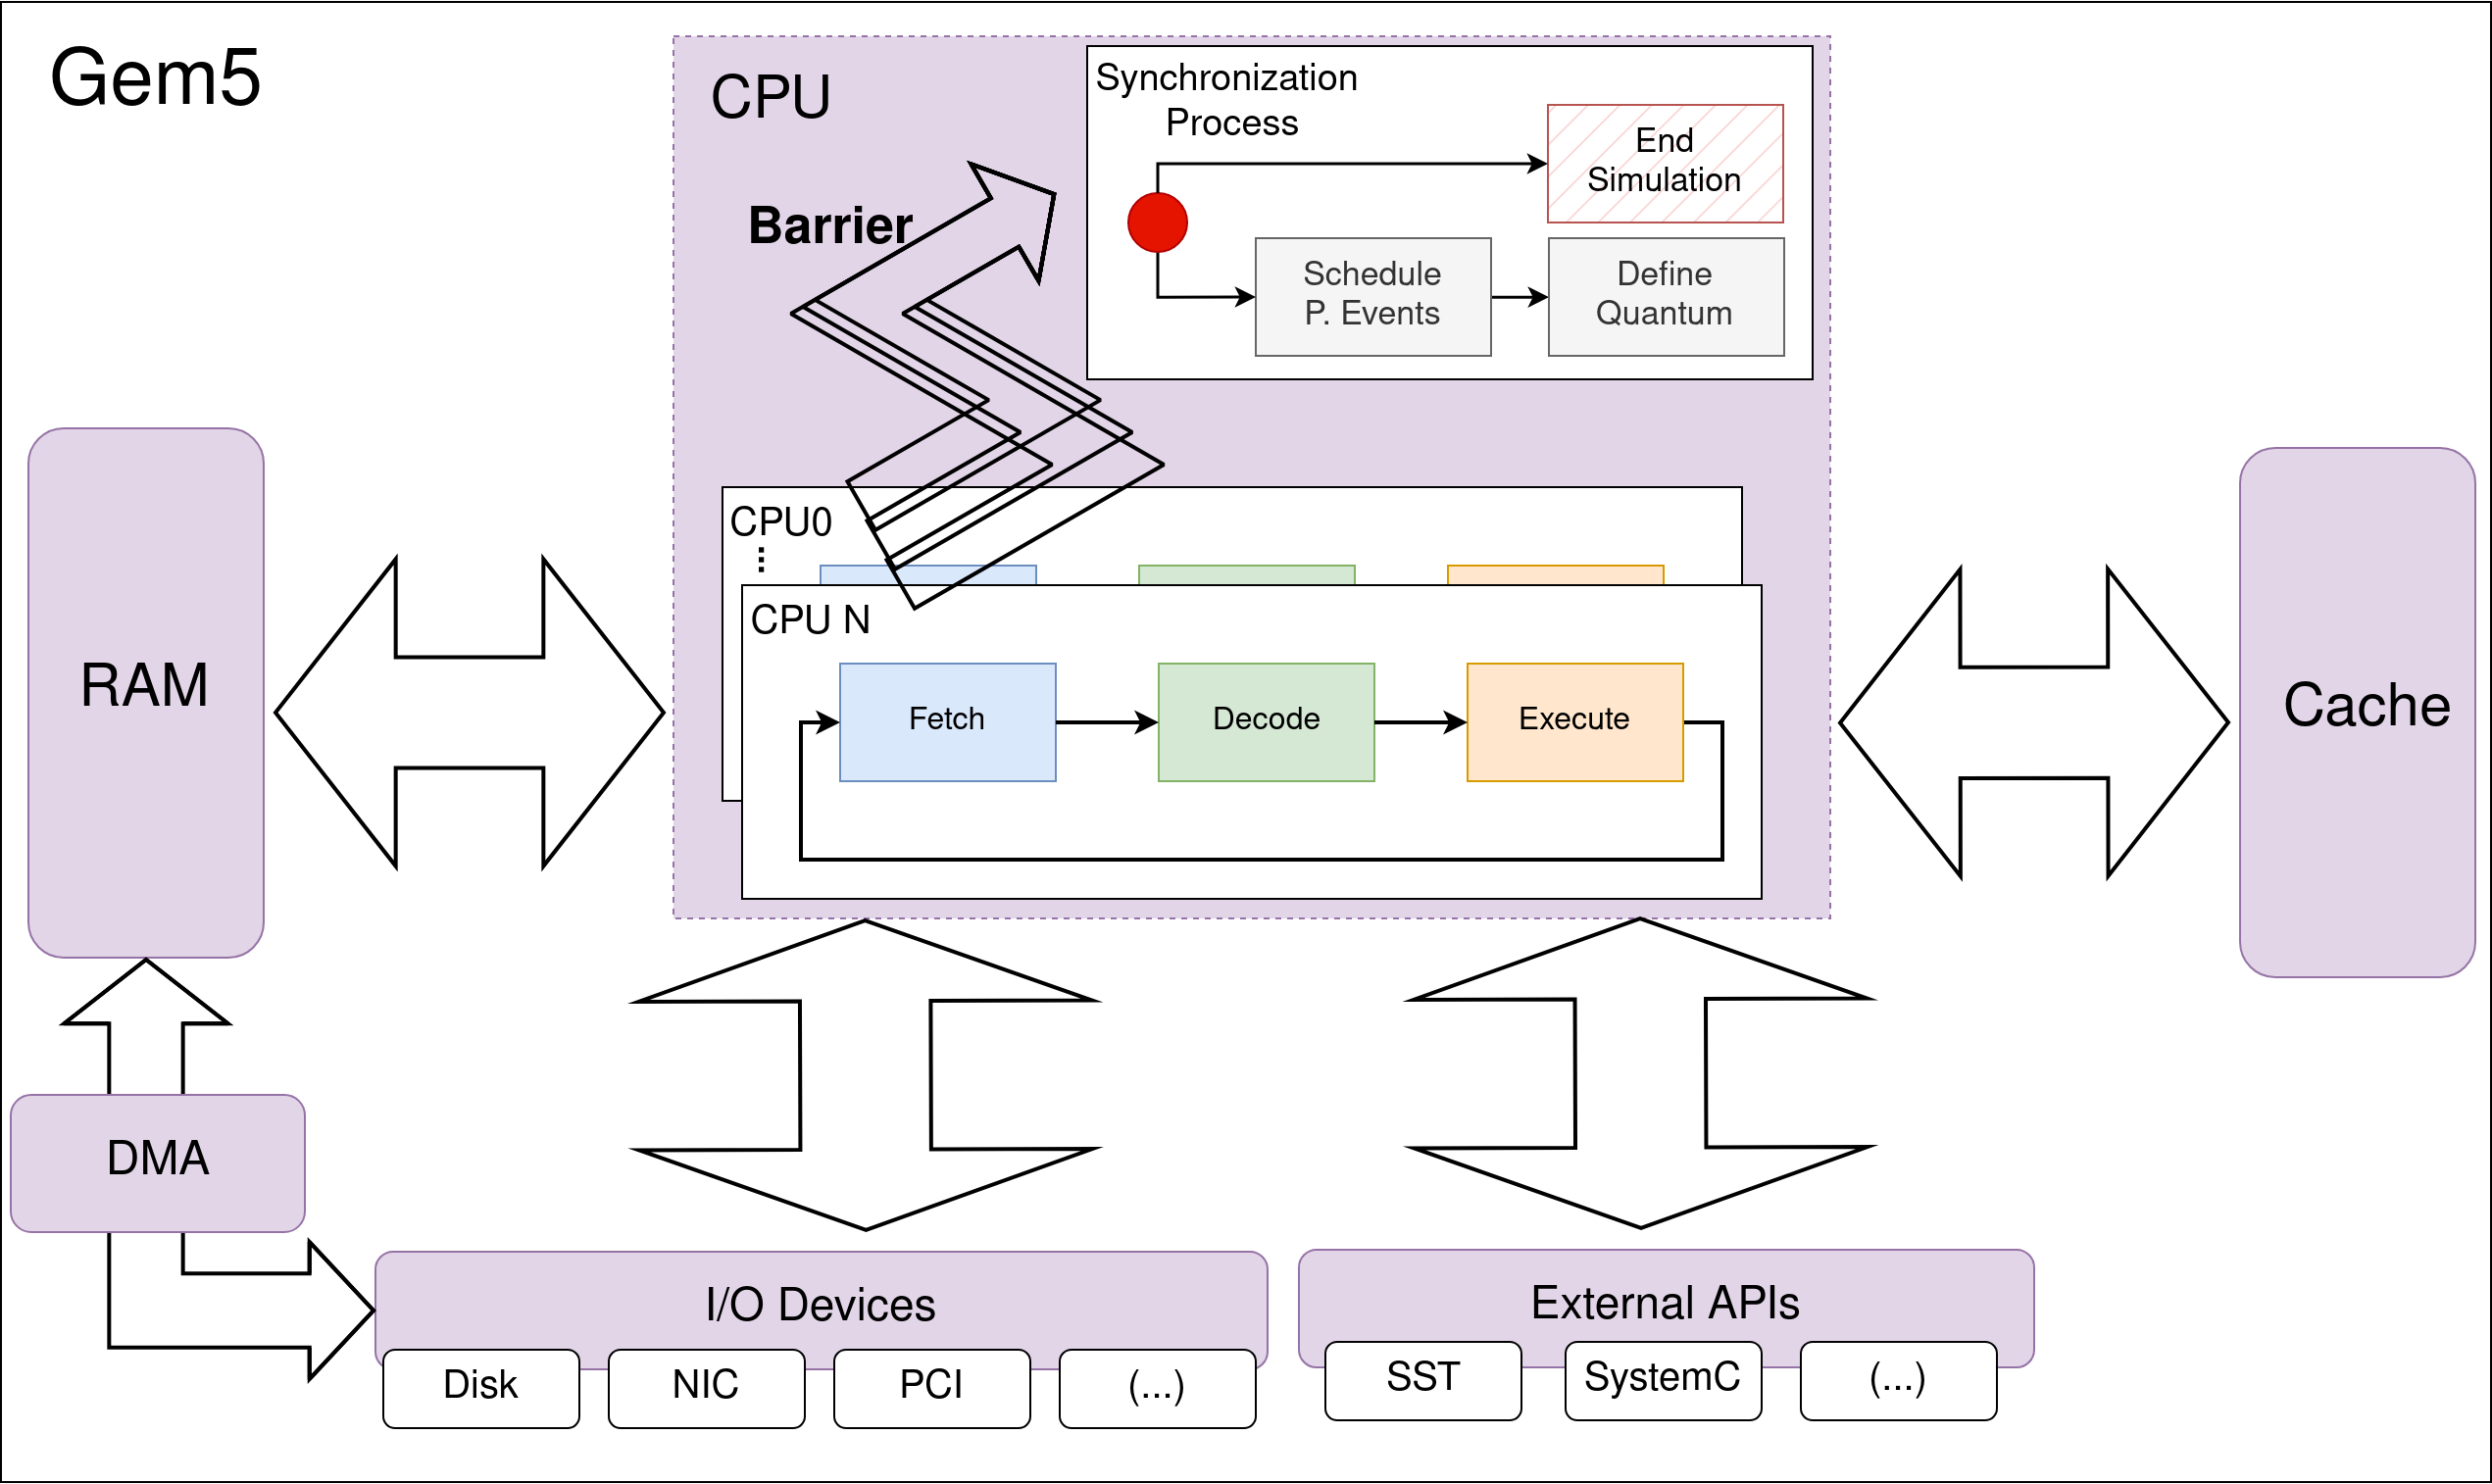
\includegraphics[width=0.8\linewidth]{Images/HighLevelPar_gem5OpMode.png}
 	\caption{High-level diagram of par-gem5 operation mode}
	\label{fig_HighLevelPar_gem5OpMode}
\end{figure}


All event queues (EQs) are running independently from each other until they reach the barrier, which is the defined time to execute 
synchronization. Due to this independence, each one has its local time thus, the processes will not hit the barrier at the same moment. 
To avoid parallelism issues, the synchronization process is only executed when all have reached the barrier. When starting this 
process, the simulator verifies if there are more events to carry out and establishes whether the simulation should continue or not.
If affirmative, the postponed events are scheduled to their respective event queues and the next synchronization is programmed for 
the current time plus the result from the developed algorithm. If not, it finishes the workload.

The first section will present an introduction to the developed extension, demonstrating the required modifications to integrate the solution and 
explaining the used benchmarks. 
After that, the remaining sections will outline the advantages and disadvantages of each algorithm, consistently comparing their performance with the 
previous scenario. In the end, an evaluation will be done, resulting in the definition of the definitive algorithm and comparing its results with 
the static version already present in the par-gem5.


\section{Par-gem5 Changes and Benchmarks}


Before going into the algorithms' design, a brief introduction about the changes in par-gem5 and the used benchmarks must be done. These changes 
were done to integrate the usage of the dynamic quantum, and to better evaluate, at the end of the simulation, its performance. 

\subsection{Par-gem5 Changes}

Two changes were made. The first was the addition of a new function mode, and the other was the inclusion of more simulation 
feedback regarding the dynamic algorithm. 

Par-gem5 has two possible simulation modes, sequential and parallel with a static quantum. When the user chooses a parallel mode, 
the simulator already knows that the quantum will not change. If the user previously provides a value, it will be applied as the new 
synchronization time otherwise, a default value is selected (1 microsecond). By adding the dynamic version, the user needs to specify a new 
parameter hence, the prior approach does not work.

Concerning this, the \textit{QuantumMode} was created to adhere to the new situation. This variable can have two states, static or 
dynamic, representing the two available versions. To integrate it into the simulator, a couple of steps were done. 
First of all, the \textit{QuantumMode} was defined and added to the list of the simulator's available types, as shown in the \autoref{SnippetParams}. 
After that, a new file was created, \autoref{SnippetQuantum}, to implement the name translation, due to the fact that the names used on the user 
side are different from the simulator side. At last, the remaining simulator was adapted to be able to select between the two versions, 
including the quantum global synchronization event, which is reasonable for the synchronization process.

\begin{lstlisting}[style=customPython, caption={Snippet of Params.py}, label=SnippetParams]
                             # (...) #
class ByteOrder(ScopedEnum):
"""Enum representing component's byte order (endianness)"""

vals = [
    'big',
    'little',
]

class QuantumMode(ScopedEnum):  
    """Enum representing quantum available modes"""

    vals = [
        '_static',
        '_dynamic'
    ]
    wrapper_name = 'QuantumMode'

# How big does a rounding error need to be before we warn about it?
frequency_tolerance = 0.001  # 0.1%
                             # (...) #
\end{lstlisting}

\begin{lstlisting}[style=customPython, caption={Quantum.py file}, label=SnippetQuantum]
import sys
from m5.util import warn
from m5.params import QuantumMode

def mode(quantum_mode):

    if(quantum_mode == "static"):
        return '_static'
    elif (quantum_mode == "dynamic"):
        return '_dynamic'
    else:
        raise TypeError("Can't convert '%s' to a quantum_mode" % type(quantum_mode))

__all__ = ['mode']
\end{lstlisting}


At the end of each simulation, par-gem5 provides a set of statistics that reflect the behavior of the performed simulation. Examples are 
the number of quanta with at least one postponed event (\textit{errQuanta}), the absolute error of par-gem5 in seconds (\textit{errSimSeconds}), 
and the number of events postponed (\textit{eventsPostponed}). However, to have a better view of how the dynamic algorithm was executed, 
the \textit{quantumMean} and \textit{DynReset} statistics were included in the final simulation results. 

The first, as the name suggests, refers to the mean of applied quantum. During the simulation, the dynamic algorithm may vary the quantum 
hence, having its average value might be useful to have an idea of how the simulation was conducted. For instance, if the workload was 
focused on performance and the \textit{quantumMean} gives a small value, it might be a sign that something went badly. The development of a 
dynamic algorithm can be another example since this data can reveal if, in some tests, the quantum was or was not the most adequate.

The \textit{DynReset} gives information about how many times the dynamic algorithm had to reset. This might happen when the dynamic system 
becomes unstable, providing illogical quantum values. Later in this chapter will be explained better this concept. 


\subsection{Benchmarks}
\label{cap:BM}

After a project development, it is common to verify if the requirements were accomplished. In this manner, the engineer 
needs to execute tests, or benchmarks, to perform the evaluation. They are designed to measure performance, capabilities, efficiency, 
and other system components. There are different types of benchmarks, each one emphasizing an area of interest. 
Some examples are \gls{cpu}, network, and storage. 

In the context of this dissertation, it will be used two \gls{cpu} benchmarks, the bare-metal bubble sort and the \gls{npb}. These will 
executed on a host and target system with the configurations exhibited in the \autoref{tab:hostSystemConfig} and \autoref{tab:targetSystemConfig}, 
respectively.
\newline

\begin{table}[!htb]
    \caption{System Configurations}
    \begin{minipage}{.5\linewidth}
      \centering
      \subcaption{Host}
        \resizebox{\textwidth}{!}{%
        \begin{tabular}{lll}
        \cline{1-2}
        \multicolumn{1}{|l|}{CPU} & \multicolumn{1}{l|}{AMD Ryzen 3990x (64 cores, 128 threads)} &  \\ \cline{1-2}
        \multicolumn{1}{|l|}{RAM} & \multicolumn{1}{l|}{128GB of 3200MHz DDR4-DRAM} &  \\ \cline{1-2}
        \multicolumn{1}{|l|}{OS} & \multicolumn{1}{l|}{Ubuntu Linux 20.04} &  \\ \cline{1-2}
         &  & 
        \end{tabular}%
        }
        \label{tab:hostSystemConfig}
    \end{minipage}%
    \begin{minipage}{.5\linewidth}
        \centering
        \subcaption{Target}
        \resizebox{\textwidth}{!}{%
            \begin{tabular}{lll}
            \cline{1-2}
            \multicolumn{1}{|l|}{CPU} & \multicolumn{1}{l|}{ARM64, AtomicSimpleCPU @ 2GHz} &  \\ \cline{1-2}
            \multicolumn{1}{|l|}{Caches} & \multicolumn{1}{l|}{64kiB L1-D, 32kiB L1-I, 2MiB L2 shared} &  \\ \cline{1-2}
            \multicolumn{1}{|l|}{Main Memory} & \multicolumn{1}{l|}{2GB of DDR3 RAM @ 1600MHz} &  \\ \cline{1-2}
            \multicolumn{1}{|l|}{Periph. Sub-system} & \multicolumn{1}{l|}{Real View Virtual Express V1} &  \\ \cline{1-2}
             &  & 
            \end{tabular}%
        }   
        \label{tab:targetSystemConfig}
    \end{minipage} 
\end{table}


\textbf{Bare-metal Bubble Sort}
\newline

The main objective of this benchmark, as implied by its name, is to rearrange an array in such a way that elements with higher values are 
positioned at the top. The algorithm employed for this task is quite straightforward. It involves a loop that iterates through the input list, 
examining each element in turn. In each iteration, the algorithm compares the current element with the subsequent one, and if the latter is 
smaller, the values are swapped. This process continues until the entire array is sorted according to the desired criterion. It was designed 
to attain a near-best-case simulation throughput, meaning that thread synchronizations and accesses to shared memory are reduced to a minimum.

\begin{figure}[H]
	\centering
 	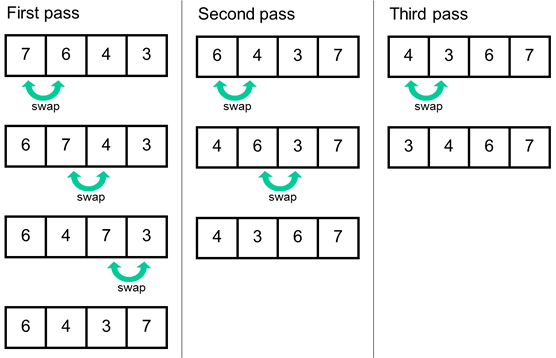
\includegraphics[width=0.7\linewidth]{Images/bubble_sort.png}
 	\caption{Bubble sort example}
	 \label{fig_bubble_sort}
\end{figure}

The test will run a pre-defined number of iterations, and 
once all the cores have completed their tasks, the simulation will conclude successfully. At the first moment, the array 
is initialized with random numbers, where the lower and bigger numbers are saved. Then, the bubble-sort 
the algorithm is executed. To ensure that the simulation ran smoothly, the program compares the first and last values of 
the sorted array with previously saved values. If there is a match, the execution is considered successful. In case of a 
mismatch, a failure is detected, and a notification is sent to the user.

This benchmark operates in a bare-metal environment, which means the program runs directly on the hardware without the mediation or 
assistance of an operating system. This approach is often chosen for 
performance-critical or resource-constrained applications where direct control over the hardware is necessary, and there is no need for the 
additional services and abstractions provided by an operating system.
\newline

\textbf{NPB}
\newline

\gls{npb} \cite{bailey1994parallel} is a group of a small set of programs designed to help the performance evaluation of parallel 
supercomputers. In total, there are eight benchmark specifications, five kernels, and three pseudo-applications. The kernel benchmarks are:

\begin{itemize}
    \item \textbf{Integer Sort (IS):} Performs a sort operation where both integer computation speed and communication performance are tested.

    \item \textbf{Fast Fourier Transform (FT):} Solves a three-dimensional partial differential equation using \glspl{fft}. 
        Long-distance communication performance is the main evaluation point. 

    \item \textbf{MultiGrid (MG):} It is a simplified multigrid kernel that requires highly structured long-distance communication. Thus, short and 
        long-distance data communications are evaluated.

    \item \textbf{Conjugate Gradient (CG):} Computes an approximation to
    the smallest eigenvalue of a large, sparse, symmetric positive definite matrix. The main goal is to test irregular long-distance communication.

    \item \textbf{Embarrassingly Parallel (EP):} It provides an estimate of the
    upper achievable limits for floating point performance, with no significant inter-process communications.
\end{itemize}

The pseudo-applications are the \textbf{Block Tridiagonal (BT)}, \textbf{Scalar Pentadiagonal (SP)}, and 
\textbf{Lower-Upper symmetric Gauss-Seidel (LU)} benchmarks. Each of these benchmarks is designed to solve a synthetic system of nonlinear partial 
differential equations using a distinct algorithm. The names of the benchmarks correspond to the specific algorithms employed in solving these 
mathematical problems.

Moreover, \gls{npb} has implemented benchmark classes that define the problem size of each workload. There are eight problem 
sizes (S, W, A, B, C, D, E, and F), where S is the smaller one and F is the bigger one. In the context of this dissertation, only the W size 
will be considered.


\section{ADALINE-Based Algorithm}

Adaptive filters are widely used due to their capacity to autonomously adjust parameters and operate with minimal or no prior 
knowledge of the signal \cite{haykin1996linear}. One application of these filters can be in the development 
of a \gls{anc} algorithm \cite{noiseCancelingADALINE}. A generic scheme can be found in the image below.

\begin{figure}[H]
	\centering
 	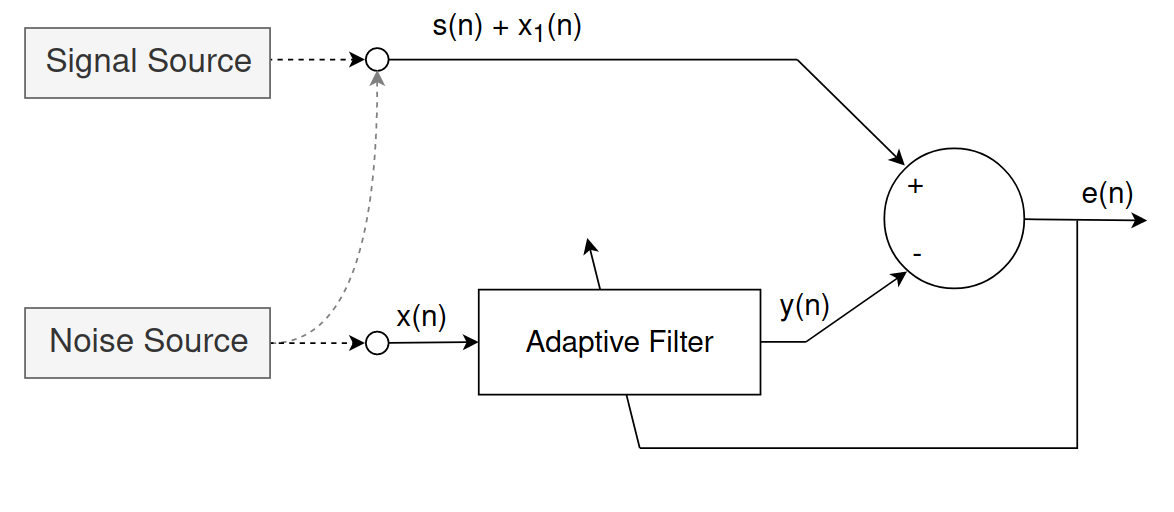
\includegraphics[width=0.7\linewidth]{Images/AdaptiveNoiseCancellationScheme.png}
 	\caption{ANC scheme}
	 \label{fig_AdaptiveNoiseCancellationScheme}
\end{figure}

While $S(n)$ is the input that has the signal mixed with the noise, $X(n)$ receives only the noise hence, it is a noise reference. If the noise 
in $S(n)$ was the same as the one presented in $X(n)$, it would only be needed to subtract the $X(n)$ to $S(n)$. Nevertheless, this noise is 
different because it is attenuated, delayed, and filtered by the noise path. For these reasons, an adaptive filter should be utilized, allowing 
$Y(n)$ to closely resemble $X_{1}(n)$. $E(n)$ will be the output without the error. It is also used by the filter in order to adapt their weights.

A comparison can be made to the par-gem5 world. The signal is the quantum, the noise is the simulation error, and the output is the quantum 
without the error. Also, the $X_{1}(n)$ and $X(n)$ are different due to the impossibility of calculate exactly $X_{1}(n)$ in runtime. When a 
benchmark is running, the simulation error obtained is referred to as the worst-case scenario. In other words, the simulator analyses when there 
is a cross-schedule event, and the time difference between when that happens and the next synchronization is considered the error since it 
is taken into account that the event must be postponed. However, most of the time, it is not true, and the event is not postponed, causing a smaller error. To 
accurately analyse what was the impact of inaccuracy ($X_{1}(n)$), it would be needed to run the sequential simulation first, killing 
all the benefits of par-gem5 \cite{pargem5}. The next equation describes how the worst-case error estimation is calculated. 

\begin{equation}
    \label{eq_errSim}
    \centering
        \Large
        e_{rel,t} = \frac{t_{sim,meas}}{t_{sim,meas}-\sum_{i=0}^{Q}t_{i,max\_pp}} -1  = \frac{t_{sim,meas}}{t_{sim,est}}-1
        \normalsize
\end{equation}
\vspace{0.3cm}

In each quantum, the postpone-mechanism records which event experienced the most significant time shift caused by the postponement, 
$t_{i,max\_pp}$. $Q$ is the number of simulated quanta and $t_{sim,meas}$ is the measured simulation time. 


\subsection{Adaptive Filter}

Following the \autoref{fig_AdalineSquematic}, the adaptive filter will be responsible for adapting the weights of the ADALINE \gls{nn}. It uses 
the \autoref{eq_LSM} for the training, where it is essential to carefully choose an appropriate learning rate.

The learning rate is a constant that is chosen at the beginning of the simulation and it is not modified. This parameter compromises a trade-off 
between control speed and stability. With lower values, the learning process is fast nevertheless, it is likely to become an unstable control 
system. With higher values, stability is granted, but the learning process is very slow, taking a lot of time to be operational.
Finding the best value is not linear, therefore an iterative approach was used. 

A small simulation was done, and in each quantum synchronization, the quantum values and the error were recorded. Furthermore, 
in this test, the quantum was incremented 1 microsecond every time a record was done. Then, the ADALINE-based algorithm was implemented in Matlab, 
obtaining the results illustrated on \autoref{fig:learningRateTests}.

\begin{figure}
\centering
\begin{subfigure}{\textwidth}
    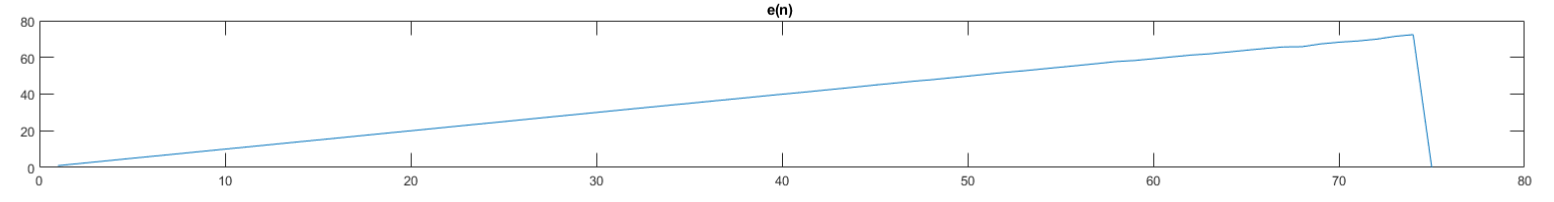
\includegraphics[width=\textwidth]{Images/AF1.png}
    \caption{ $\mu = 1 * 10^{-16} $ }
    \label{fig:AF1}
\end{subfigure}
\begin{subfigure}{\textwidth}
    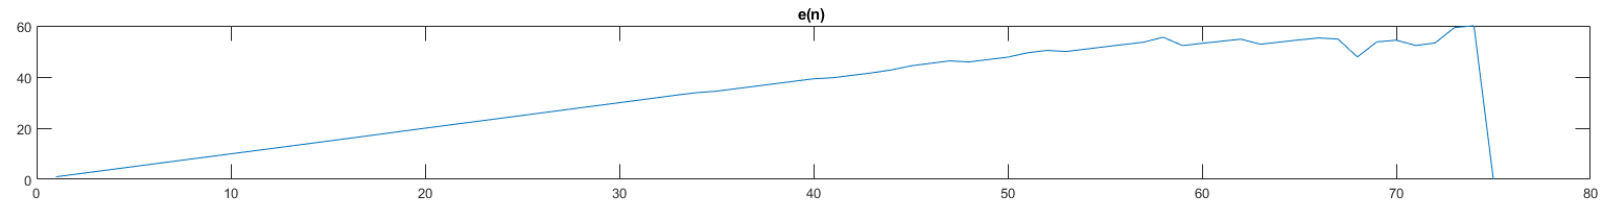
\includegraphics[width=\textwidth]{Images/AF2.png}
    \caption{ $\mu = 1 * 10^{-17}$ }
    \label{fig:AF2}
\end{subfigure}
\begin{subfigure}{\textwidth}
    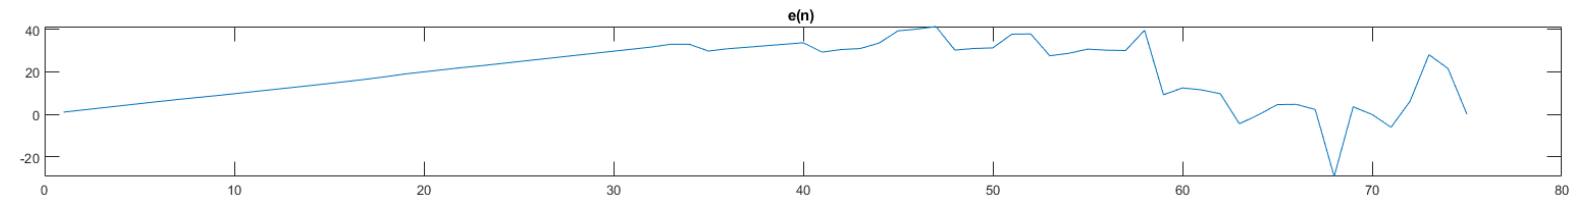
\includegraphics[width=\textwidth]{Images/AF3.png}
    \caption{ $\mu = 1 * 10^{-18}$ }
    \label{fig:AF3}
\end{subfigure}
        
\caption{Control action with different learning rate values}
\label{fig:learningRateTests}
\end{figure}

 The aforementioned mention trade-off can be observed, where for $\mu > 1 * 10^{-16} $, the results were similar to \autoref{fig:AF1}, and 
 for $\mu < 1 * 10^{-18} $, the system become even more unstable. To choose the learning rate, the logarithmic scale is used, as small variations 
 in the $\mu$ do not result in a significant change. From the results was concluded that the best value for $\mu$ is $1 * 10^{-17}$. 

Although on this test when $\mu$ was equal to $1 * 10^{-17}$ did not result in an unstable control system, there is a possibility that it could 
happen, for example, when there are huge error variations. Typically, these variations occur when the synchronization time is much longer than the 
ideal case, which requires resetting the algorithm. Regarding the results on \cite{pargem5}, where it was observed the inaccuracy grows with 
increasing quantum and number of cores, it was also implemented a \textit{safeQuanta}, a value that is smaller than the actual quantum. It depends 
on the previously mentioned characteristic, that is, when more cores are being simulated, this value becomes smaller. 
The next flowchart illustrates how the reset system works.

\begin{figure}[H]
	\centering
 	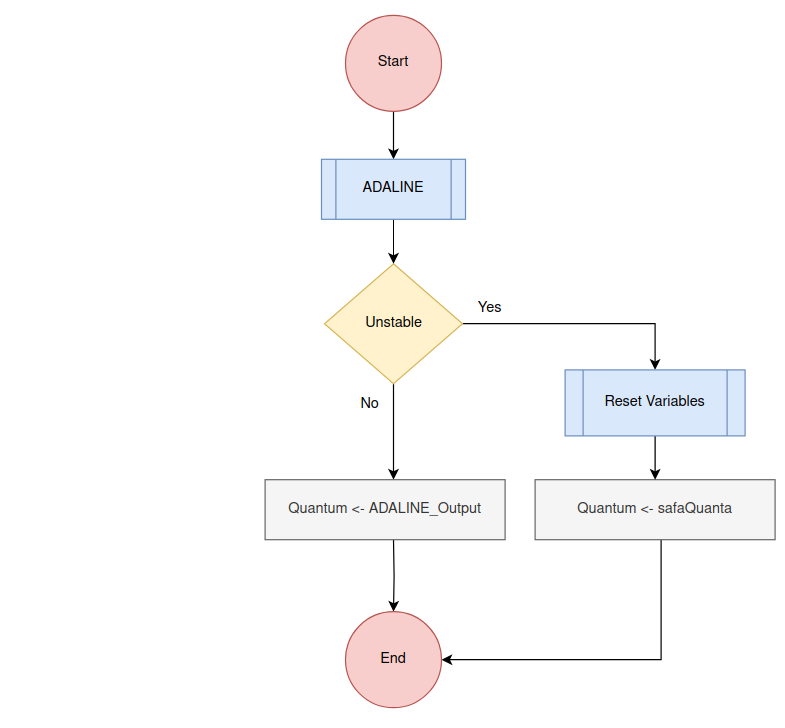
\includegraphics[width=0.6\linewidth]{Images/ResetSystemADALINE.png}
 	\caption{Reset system in ADALINE-based algorithm}
	 \label{fig_ResetSystemADALINE}
\end{figure}

If the ADALINE output is negative, means it became unstable, and a reset is required. In the reset, all the variables used in the calculation are set 
into their initial conditions. Although it will sacrifice simulation performance, this action is lightweight, meaning a negligible variation. 
Yet, it is desirable to have the least resets possible.

\subsection{TDL}

As the simulation precedes, there is more data to analyse, taking away performance from the \gls{nn}. Stella et al. \cite{noiseCancelingADALINE} 
presented one example of an application where this problem is also present. The solution to make full use of the ADALINE network as an adaptive 
filter was the implementation of a \gls{tdl}. Its operating method is described in the figure below. 

\begin{figure}[H]
	\centering
 	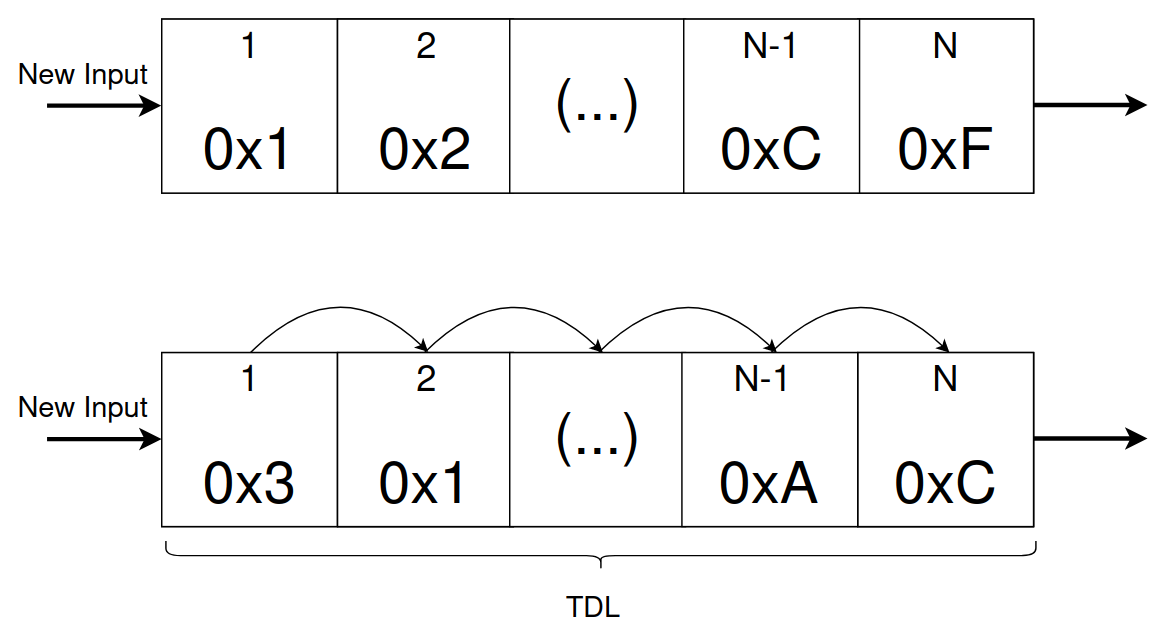
\includegraphics[width=0.5\linewidth]{Images/TDL.png}
 	\caption{TDL working method}
	 \label{fig_TDL}
\end{figure}

One input is considered $N$ times, being $N$ the size of the \gls{tdl}. When a new input arrives, the oldest one is discarded. In the end, 
the \gls{tdl} have always the signal at the current time, the previous input signal, and so on. Combining the \gls{tdl} with the ADALINE, 
efficiency and performance are no longer sacrificed. This approach was implemented in the noise source since it receives new data in each new 
quantum evaluation. 

\gls{tdl} size varies from application to application. In this case, when the size is small, the learning process may be subpar, but it also 
becomes less sensitive to variations in the noise. In contrast, a larger size leads to more effective weight adjustments through improved learning, 
but it makes the \gls{nn} more susceptible to noise variations. To choose the best size for this scenario, a small test was done where different 
\gls{tdl} sizes were utilized. The results are presented in the following graph.

\begin{figure}[H]
	\centering
 	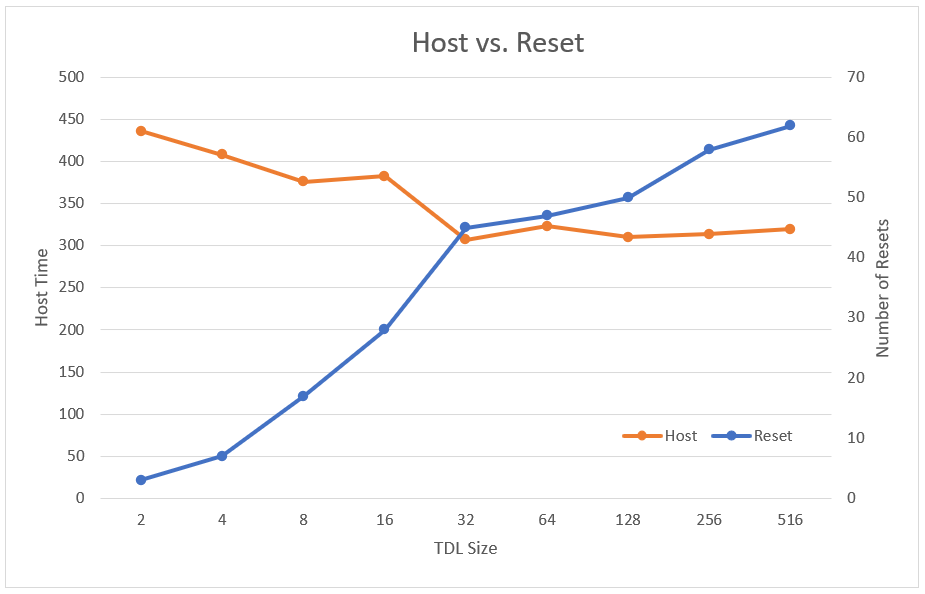
\includegraphics[width=0.7\linewidth]{Images/ResetVsHost.png}
 	\caption{Reset vs. Host}
	 \label{fig_ResetVsHost}
\end{figure}

To have maximum performance on the simulator, only base $2^{n}$ sizes were chosen, where $n \in N$. Observing the outcome, it can be seen that 
there is a point where the host time does not improve significantly however, the number of resets continues increasing. As previously noted, 
each reset has a 
performance impact, as it requires resetting every variable to its initial conditions. Therefore, it is desirable to minimize the number of 
resets whenever possible. In conclusion, the best size to be used is 32, and for this reason, it was used for the subsequent 
tests.

\subsection{Quantum Increment}

The ADALINE-based algorithm output, that is, the filtered quantum, will be always lower than the source. Using this new quantum implies there will 
be a point in time when it becomes too small, primarily because it fails to increase its value. This situation inevitably leads to a 
trade-off, wherein performance is compromised. To strike the optimal balance, it becomes necessary to increment the quantum value. This adjustment 
should occur when no errors are detected in the system. \autoref{fig_ADALINE_v1} presents the flowchart for the ADALINE-based algorithm.

\begin{figure}[H]
 	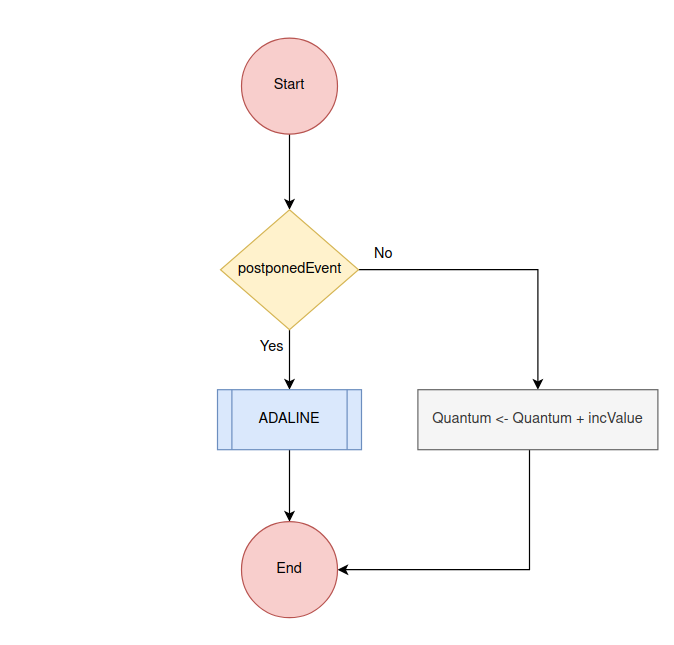
\includegraphics[width=0.32\linewidth]{Images/ADALINE_v1.png}
 	\caption{ADALINE flowchart}
	 \label{fig_ADALINE_v1}
\end{figure}

When an event must be postponed, it is considered that an inaccuracy problem occurred, indicating that the quantum should be reduced. In 
the synchronization state, the first step is to verify the preceding scenario and determine whether the quantum is incremented or the 
ADALINE-based algorithm takes action.

The increment value should have a balance, in the way that with a smaller increment, the performance may not be improved, and 
with a high value the accuracy may be ruined. According to \cite{pargem5}, the quantum of 1 microsecond gives a good trade-off between those 
two thus, it was chosen to use an increment 10 times lower. This value enables a significant balance without causing any harm.

\subsection{Results}
\label{sec:ADALINE_results}

The aforementioned benchmarks executed the developed algorithm with different numbers of cores. The results obtained are depicted in the 
\autoref{fig:results_ADA}. 

\begin{figure}[]
\centering
\begin{subfigure}{\textwidth}
    \centering
    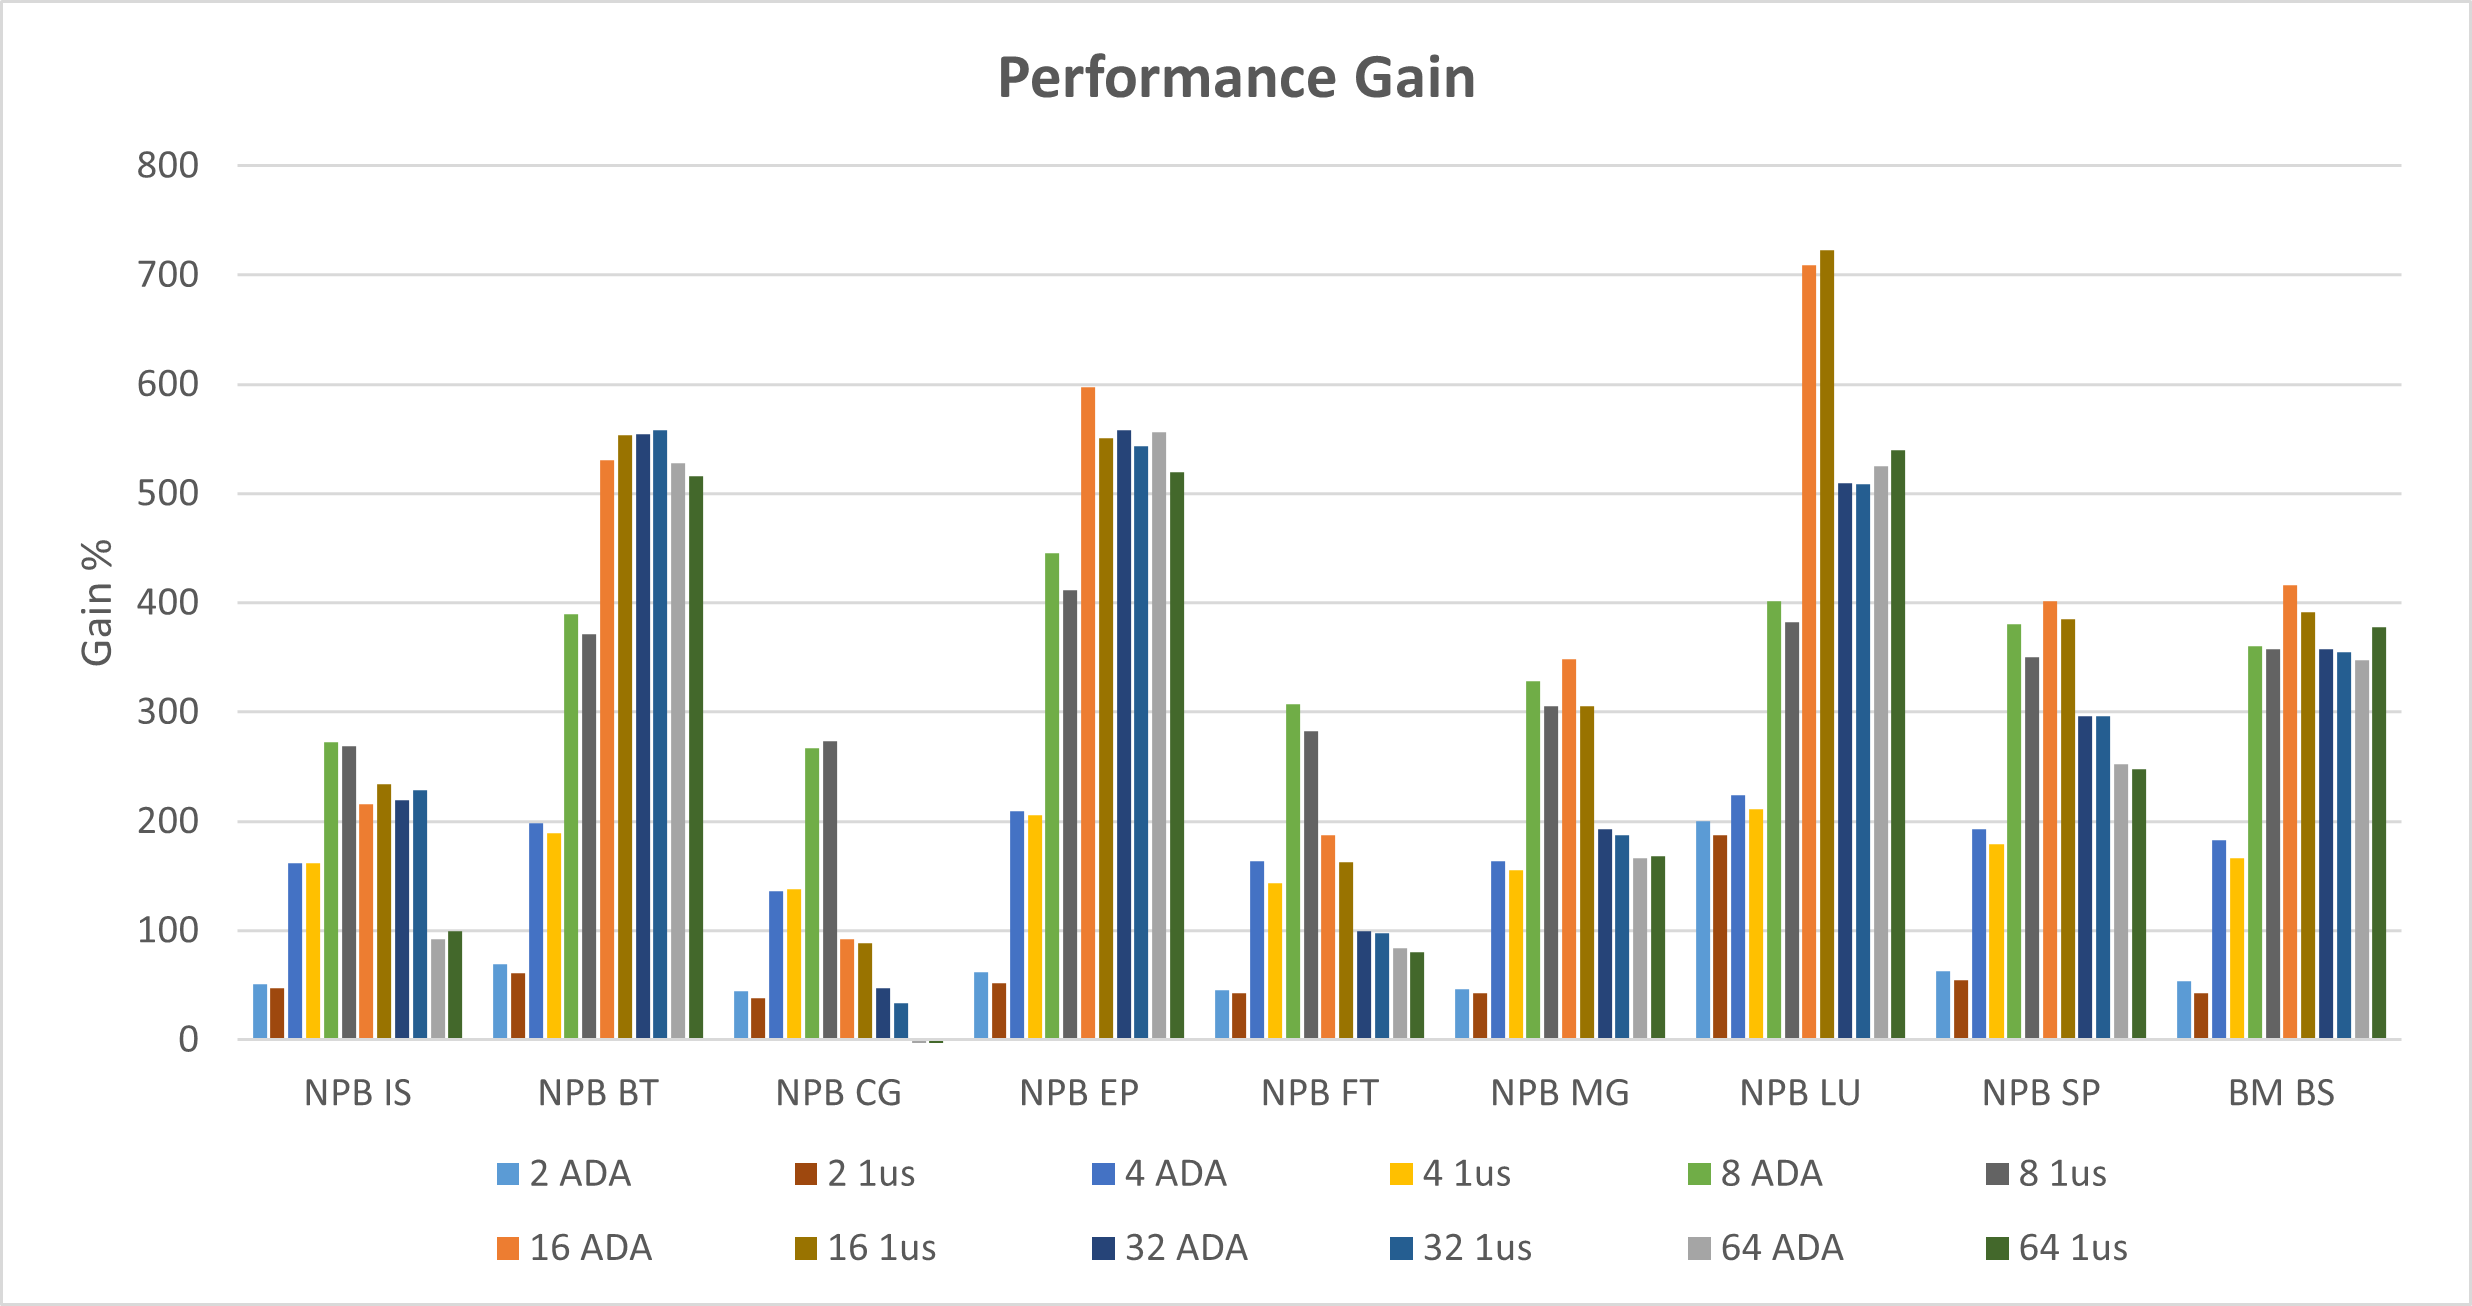
\includegraphics[width=0.8\textwidth]{Images/Performance_ADA.png}
    \caption{ Performance gain}
    \label{fig:Performance_ADA}
\end{subfigure}
\begin{subfigure}{\textwidth}
    \centering
    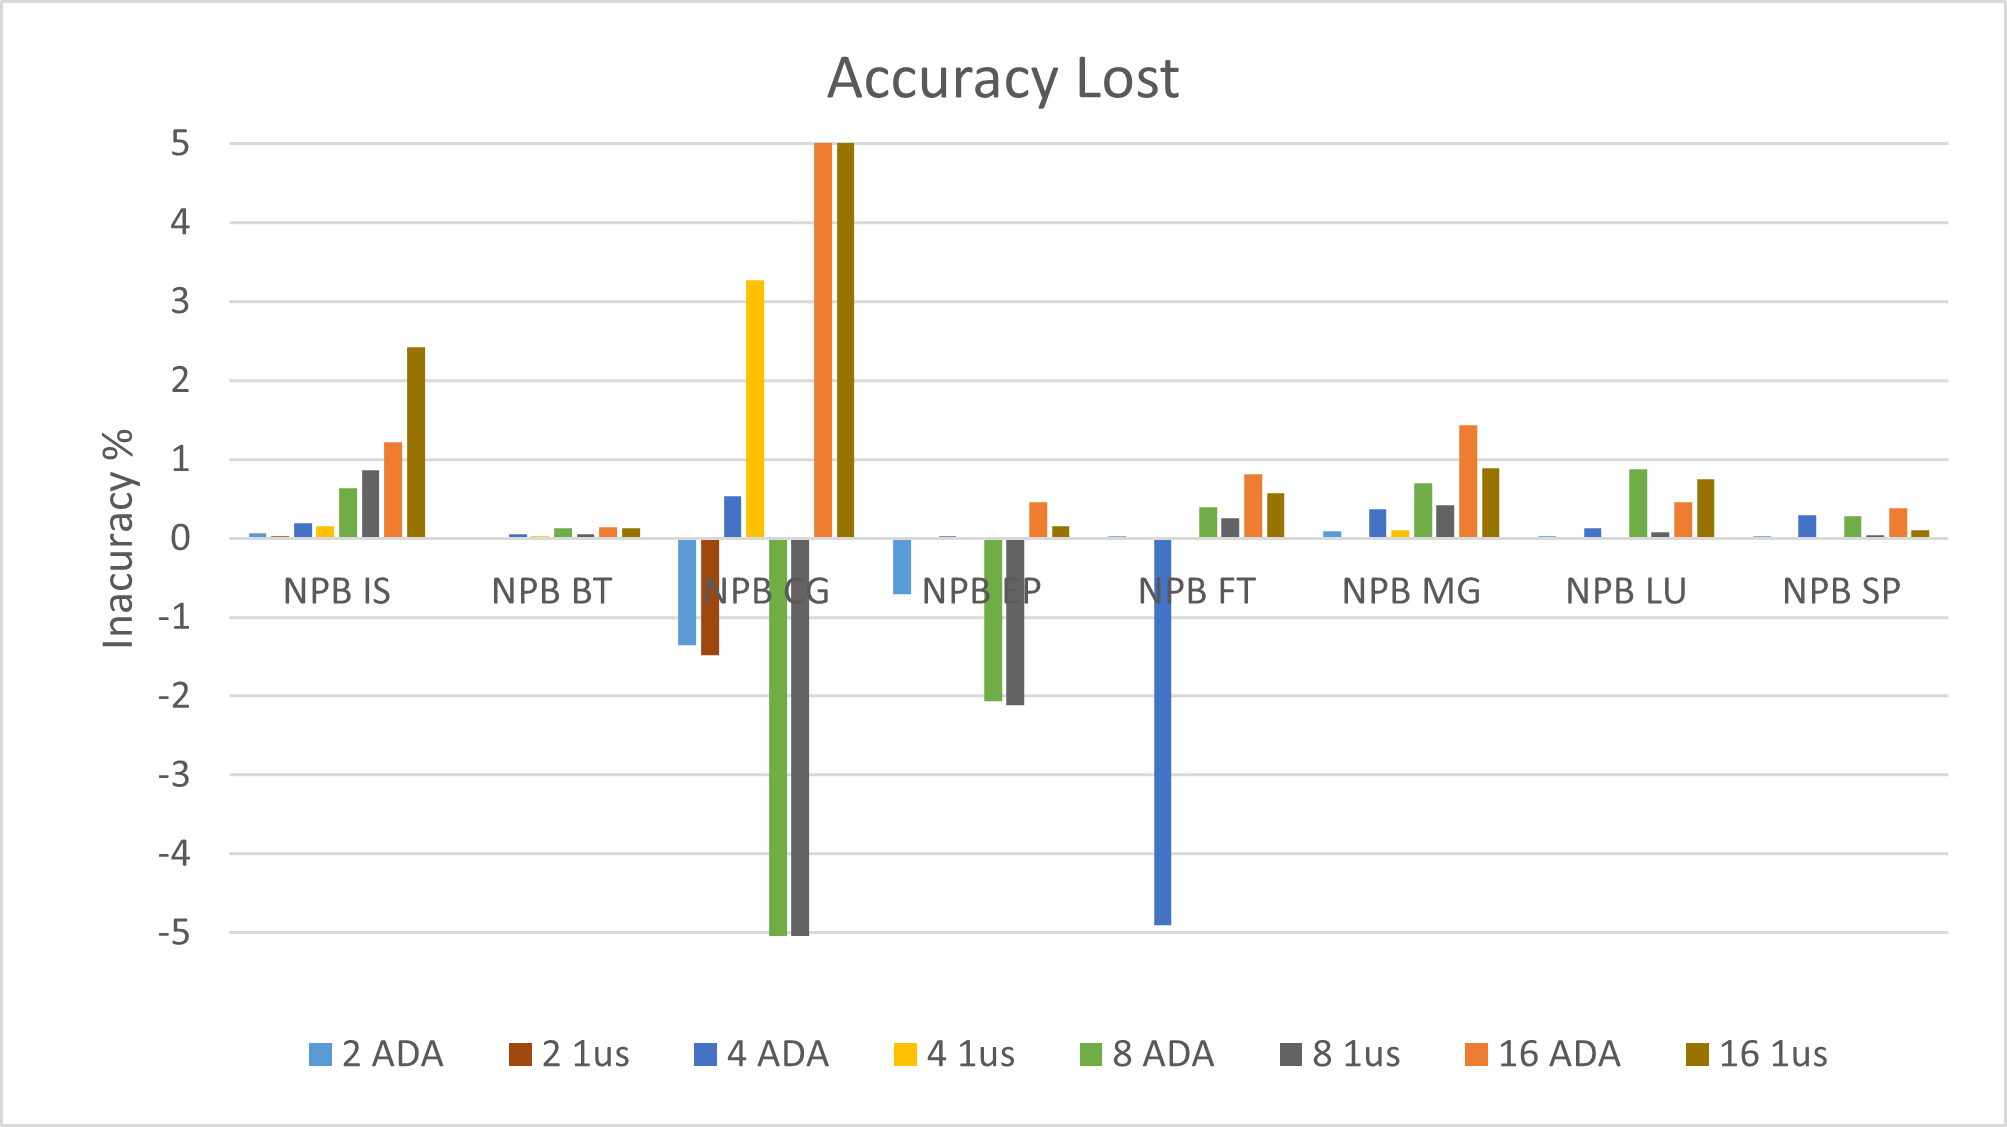
\includegraphics[width=0.8\textwidth]{Images/Accuracy_ADA.png}
    \caption{ Accuracy lost}
    \label{fig:Accuracy_ADA}
\end{subfigure}
\begin{subfigure}{\textwidth}
    \centering
    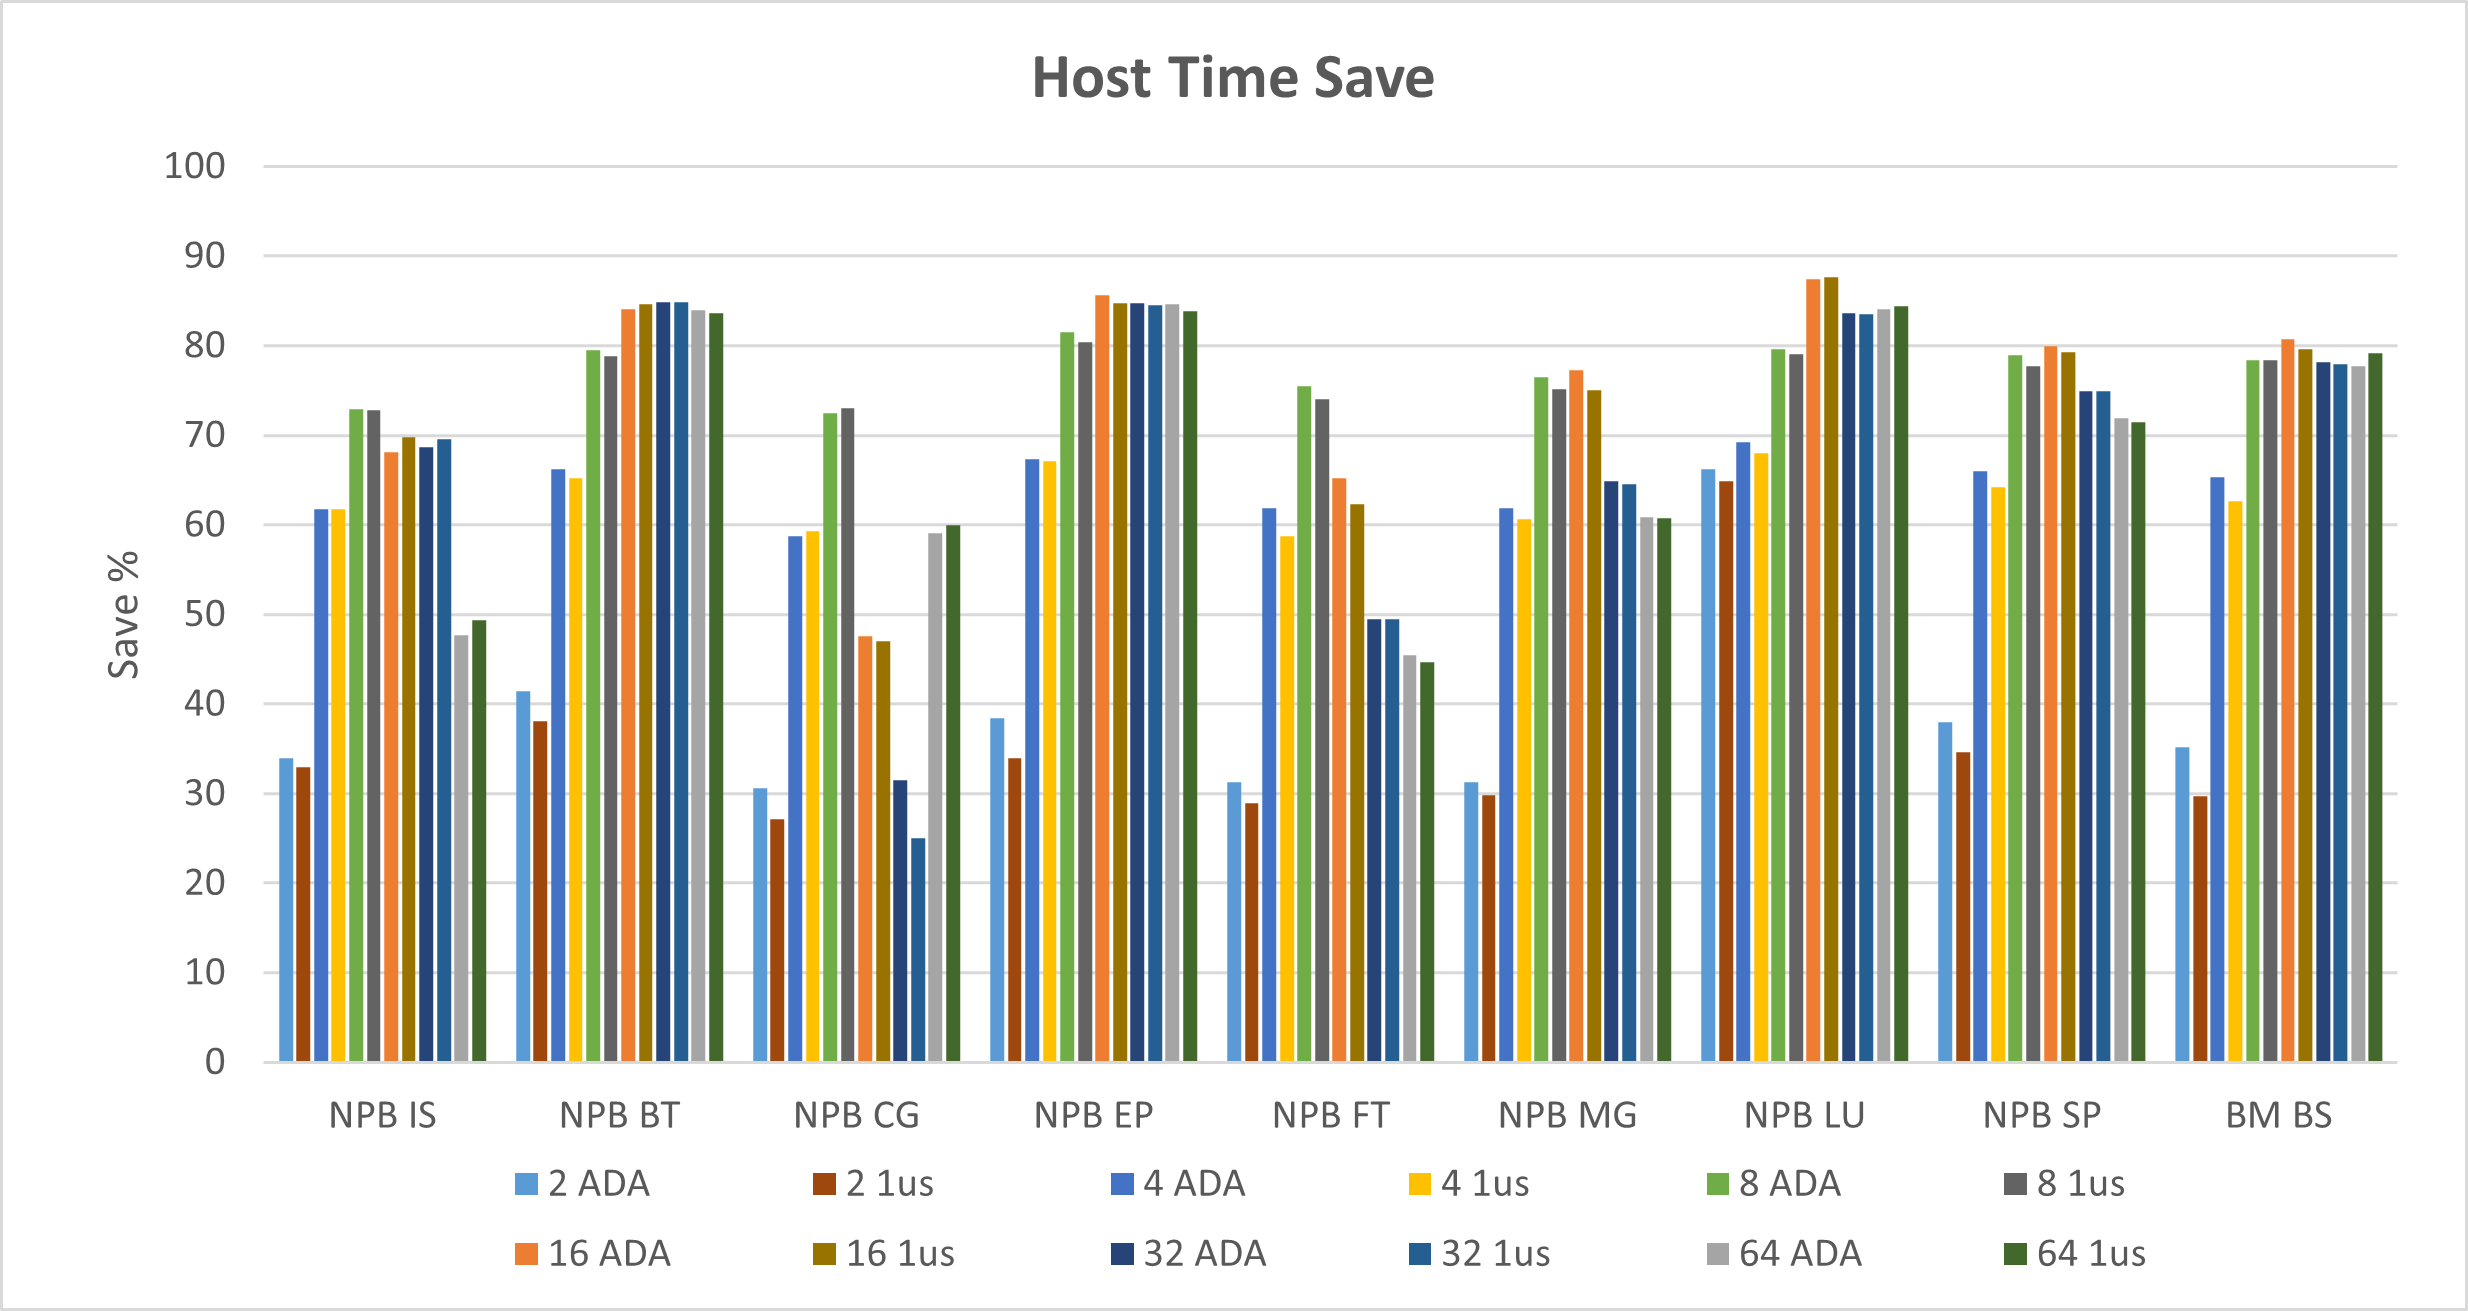
\includegraphics[width=0.8\textwidth]{Images/Host_ADA.png}
    \caption{ Host time save}
    \label{fig:Host_ADA}
\end{subfigure}
        
\caption{ADALINE-based algorithm results}
\label{fig:results_ADA}
\end{figure}

The horizontal subtitle illustrates the executed benchmark along with the number of cores and the corresponding algorithm used, hence 4 ADA 
means four cores with the ADALINE-based algorithm were simulated. To assess the ADALINE performance, the static version was also executed with 
a quantum set to one microsecond. In all cases, the comparison reference is the result obtained from sequential simulation. Additionally, the 
results for a single simulated core are not presented because, in all conducted tests, the sequential simulation exhibited similar performance. 
Hence, this scenario is not relevant for evaluating the algorithms.

When it comes to performance, it is noticeable that the algorithm yielded better results in certain benchmarks such as bare-metal, NPB EP, and SP. 
However, in other cases like NPB IS and CG, it did not show significant improvements. Shifting the focus to accuracy, the static version generally 
outperformed the dynamic approach. Nevertheless, it systematically maintained an accuracy of under 2\%, with the exception of some cases, like
NPB CG, where both approaches performed poorly. Lastly, when comparing the host time to performance, similar outcomes were observed, though 
certain benchmarks exhibited superior results to others.

Concerning the \autoref{fig_SchedulingEventGem5}, it can be stated that the target time obtained with the parallel mode can only 
be higher than the one obtained with the sequential mode. Two reasons justify the previous sentence. The first one is related to 
\gls{td}, where its use may cause a higher target time due to the obligation of only ending the simulation in the synchronization process. 
The second one is connected to postponed events since these may delay the simulation. For these reasons, inaccuracy can only be positive.
Nevertheless, as shown on the graph, this is not the case. It is worth mentioning that these occurrences are not related to 
the algorithm itself but rather to par-gem5, as simulation with the static version also evidences this dilemma.

The performance issue may be related to the previous quantum increment consideration. It is clear this value for some workloads is good, but 
for others may not be the most adequate. Therefore, having a dynamic value would solve this problem, resulting in a more flexible algorithm. 
Moreover, special attention should be given to its design, as excessively large values can lead to an unfavorable trade-off.


\section{Step Ladder Algorithm}

As shown, it was verified in some cases where the performance was equal or lower when compared with the static approach. Concerning the quantum 
increment, a fixed value was defined following the aforementioned philosophy however, a dynamic approach may bring better results, as different 
benchmarks require different needs. 

Therefore, the ADALINE-based algorithm was updated to integrate this new functionality. Observing the \autoref{fig_ADALINE_v1}, the calculation of the 
increment value (\textit{incValue}) will be done before the if statement, so whether there is a postponed event or not, the \textit{incValue} is always controlled. 
The new flowchart is represented in the next figure.

\begin{figure}[H]
	\centering
 	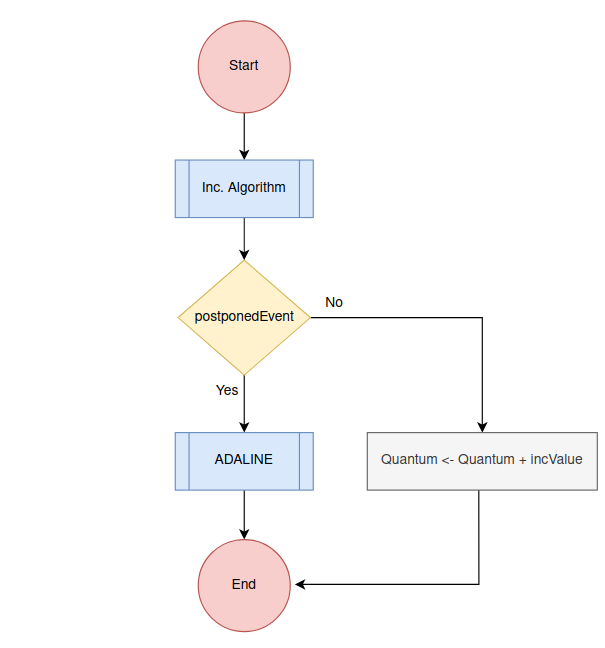
\includegraphics[width=0.32\linewidth]{Images/ADALINE_v2.png}
 	\caption{ADALINE-based and Step Ladder algorithms combined}
	 \label{fig_ADALINE_v2}
\end{figure}

The concept is to initiate with a gradual increase in value initially. If there are no postponed events during this period, then the increment 
can be escalated. It can be seen as an exponential however, an approach like this would scale too fast, affecting the accuracy. A solution can be 
the definition of a threshold, where the increment value only increases if no "accuracy issues" have happened N times in a row. An example is 
illustrated in the \autoref{fig_incAlgorithm_graph}. It is possible to observe that there is a point, marked in red, 
where there was no variation in the \textit{incValue}, indicating the occurrence of a postponed event.

\begin{figure}[h!]
	\centering
 	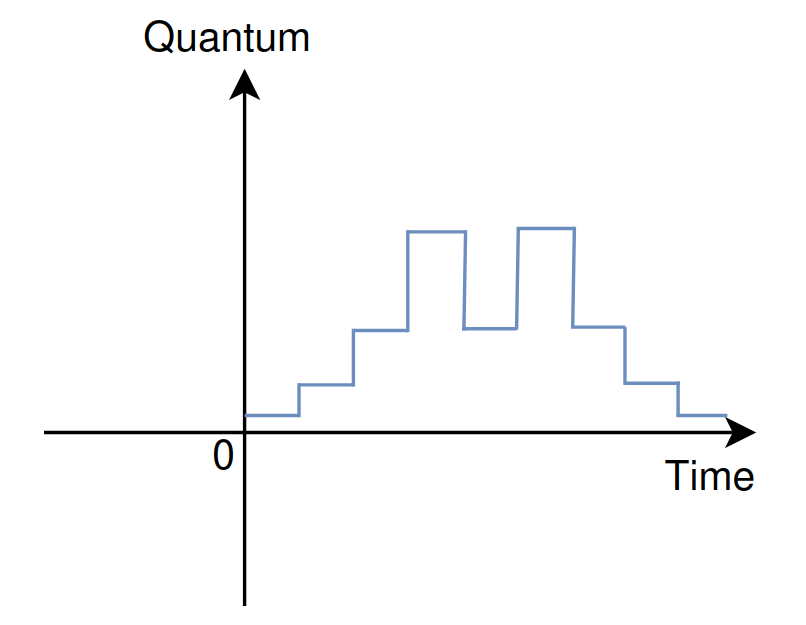
\includegraphics[width=0.4\linewidth]{Images/incAlgorithm_graph.png}
 	\caption{Example of the increment value evolution with a threshold}
	 \label{fig_incAlgorithm_graph}
\end{figure}

The \textit{incValue} starts in the smaller value possible (\textit{minValue}), which is equal to the clock period, 
and can grow until a maximum (\textit{maxValue}) of a hundred microseconds.  
This value was defined regarding the results on \cite{pargem5} and \cite{BeyondQuantumTDSim}, where the benefits of a 
quantum of this magnitude are few. The addition method respects the subsequent equation.

\begin{equation}
    \label{eq_incValue}
    \centering
        \Large
        incValue = 2 * incValue
        \normalsize
\end{equation}
\vspace{0.3cm}

Oppositely, the decrement is done by dividing by two the actual \textit{incValue}, until it reaches the minimum. The threshold value depends on how 
many cores are used by the simulation since the inaccuracy grows with the increasing number of cores. The more cores are being used, the greater 
the threshold, making it harder to increase the \textit{incValue}. Moreover, the increment value only changes (increases or decreases) if it 
fulfills the condition for N consecutive times, as shown in the later image. 

The algorithm starts checking if any event 
was postponed. If yes, it is considered that an "inaccuracy problem" occurred. If not, it is considered that the quantum value was the right one.
Then, the \textit{maxCondition} and \textit{minCondition} ensure that the \textit{incValue} does not cross the previously set boundaries. To control the 
increment or decrement sequence, it was created the \textit{incIndex} and \textit{decIndex}, respectively, These are incremented or reset, as 
shown in the subsequent flowchart, and they are used to check if the increment or decrement threshold has been reached.

\begin{figure}[H]
	\centering
 	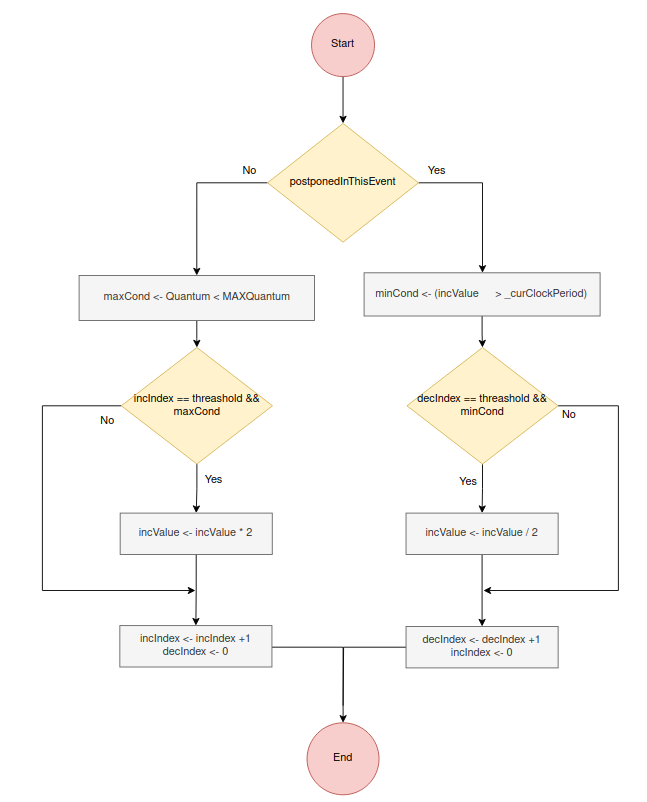
\includegraphics[width=0.6\linewidth]{Images/incAlgorithm_flowchart.png}
 	\caption{Step Ladder algorithm flowchart}
	 \label{fig_incAlgorithm_flowchart}
\end{figure}

\subsection{Results}

The previous benchmarks executed the new approach with different numbers of cores. The results obtained are depicted in the 
\autoref{fig:results_ADAINC}. 

\begin{figure}[H]
\centering
\begin{subfigure}{\textwidth}
    \centering
    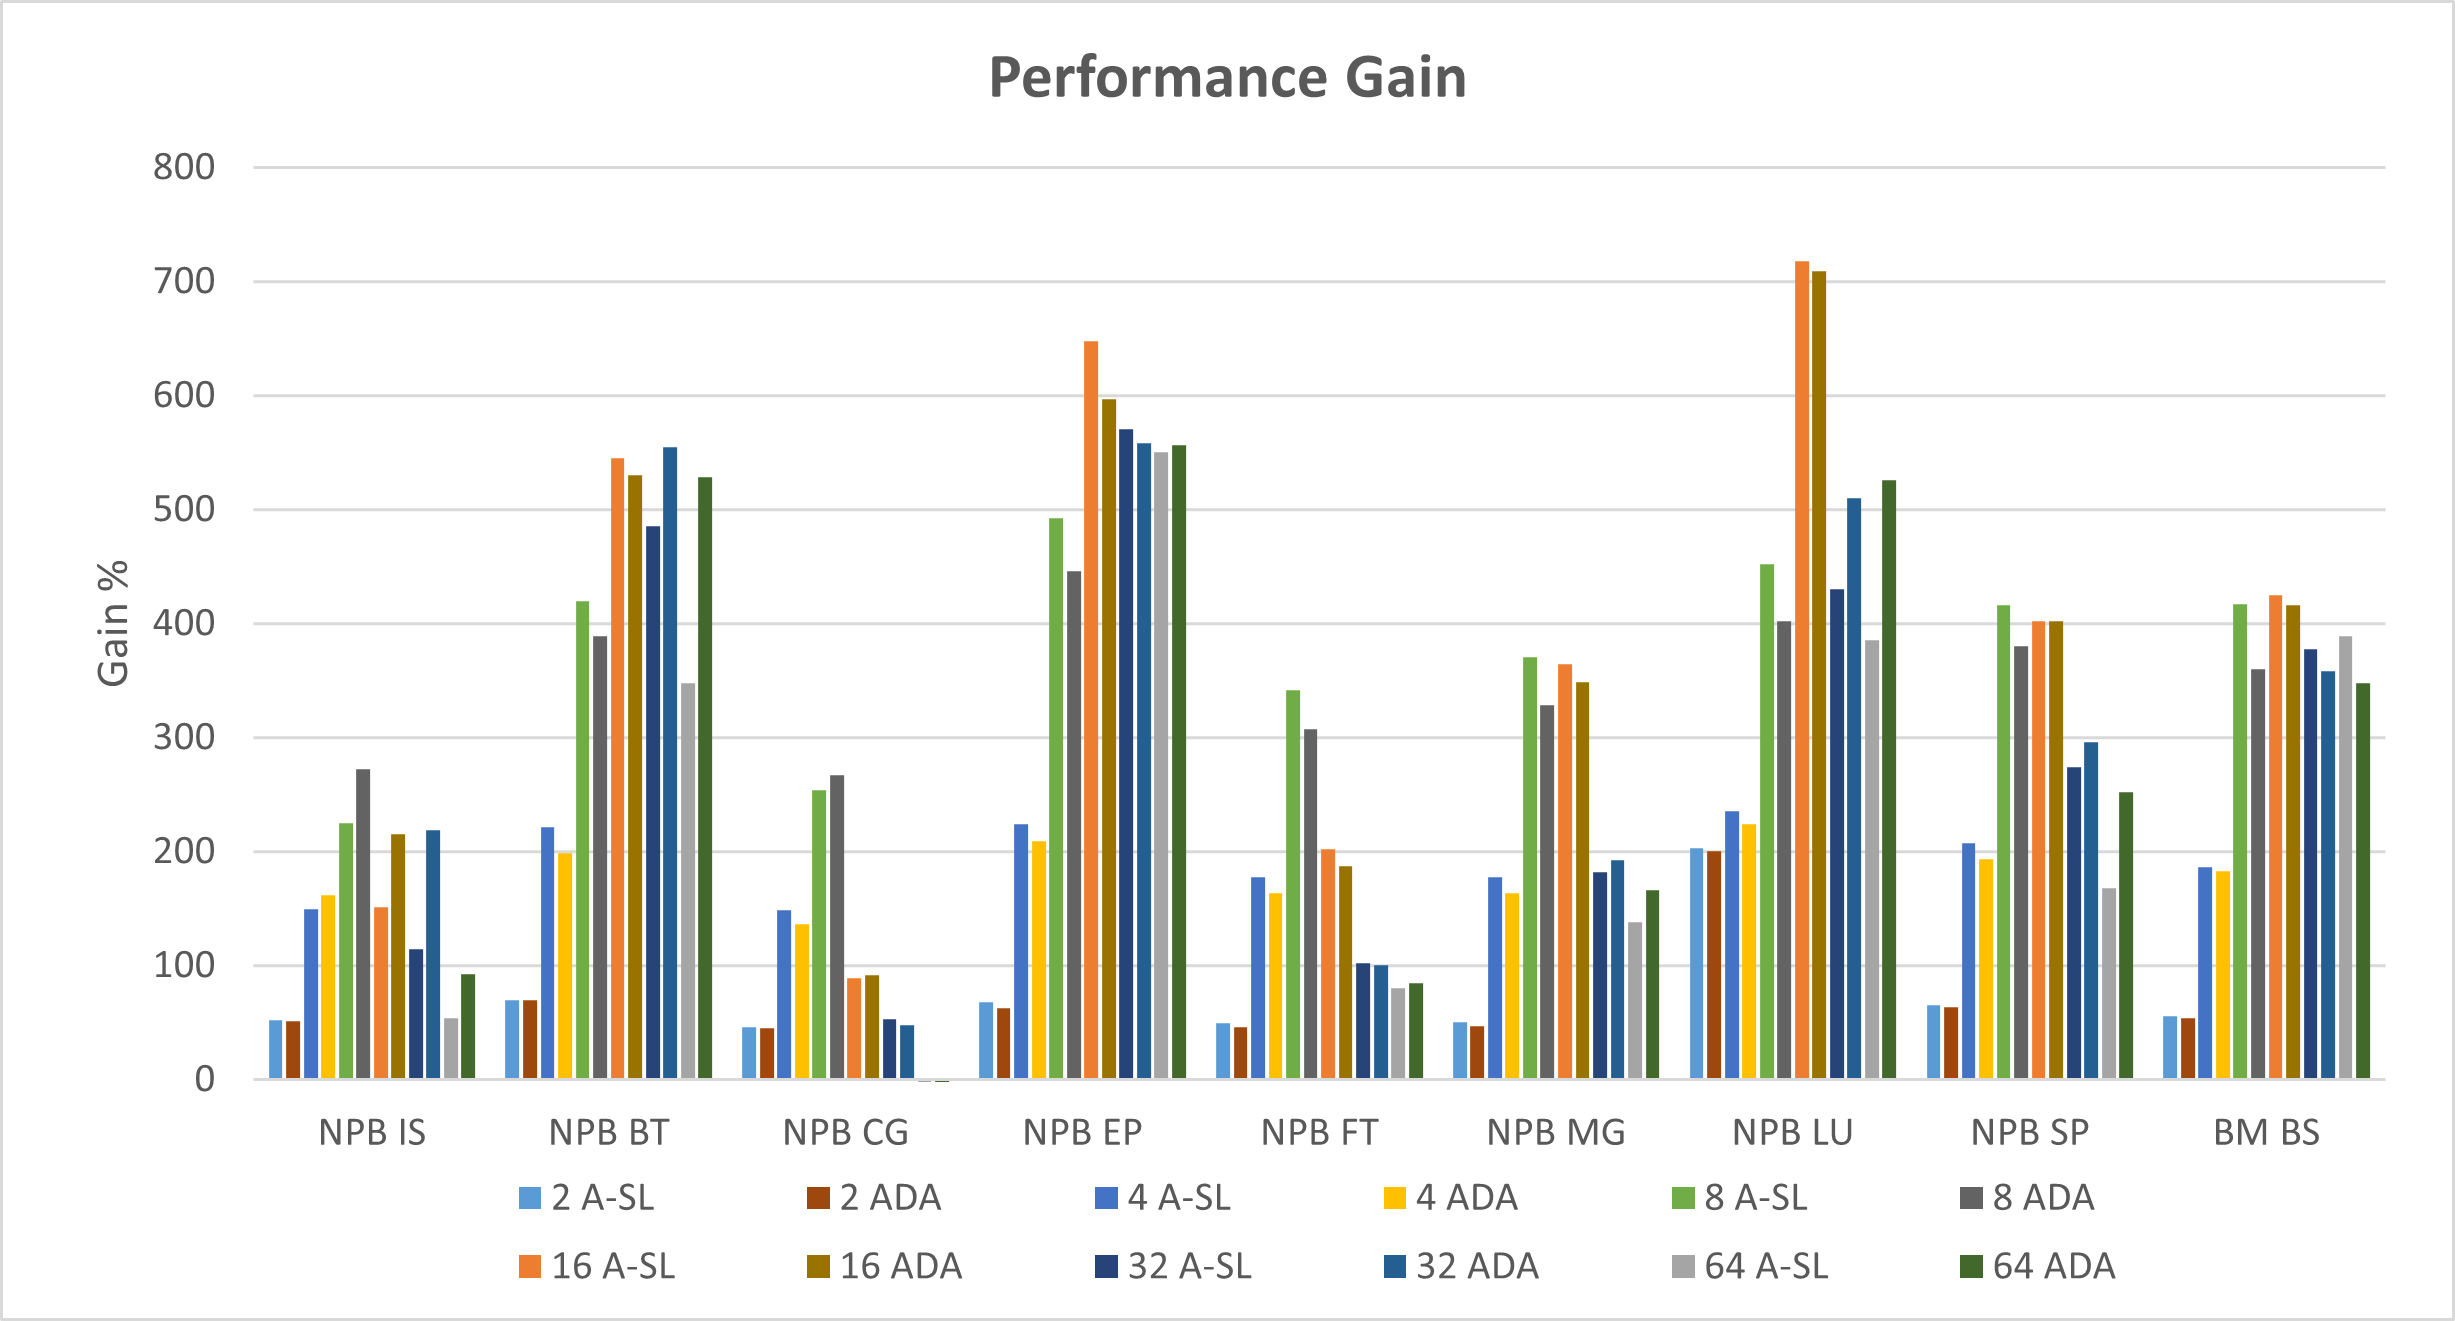
\includegraphics[width=0.8\textwidth]{Images/Performance_ADA_INC.png}
    \caption{ Performance gain}
    \label{fig:Performance_ADAINC}
\end{subfigure}
\begin{subfigure}{\textwidth}
    \centering
    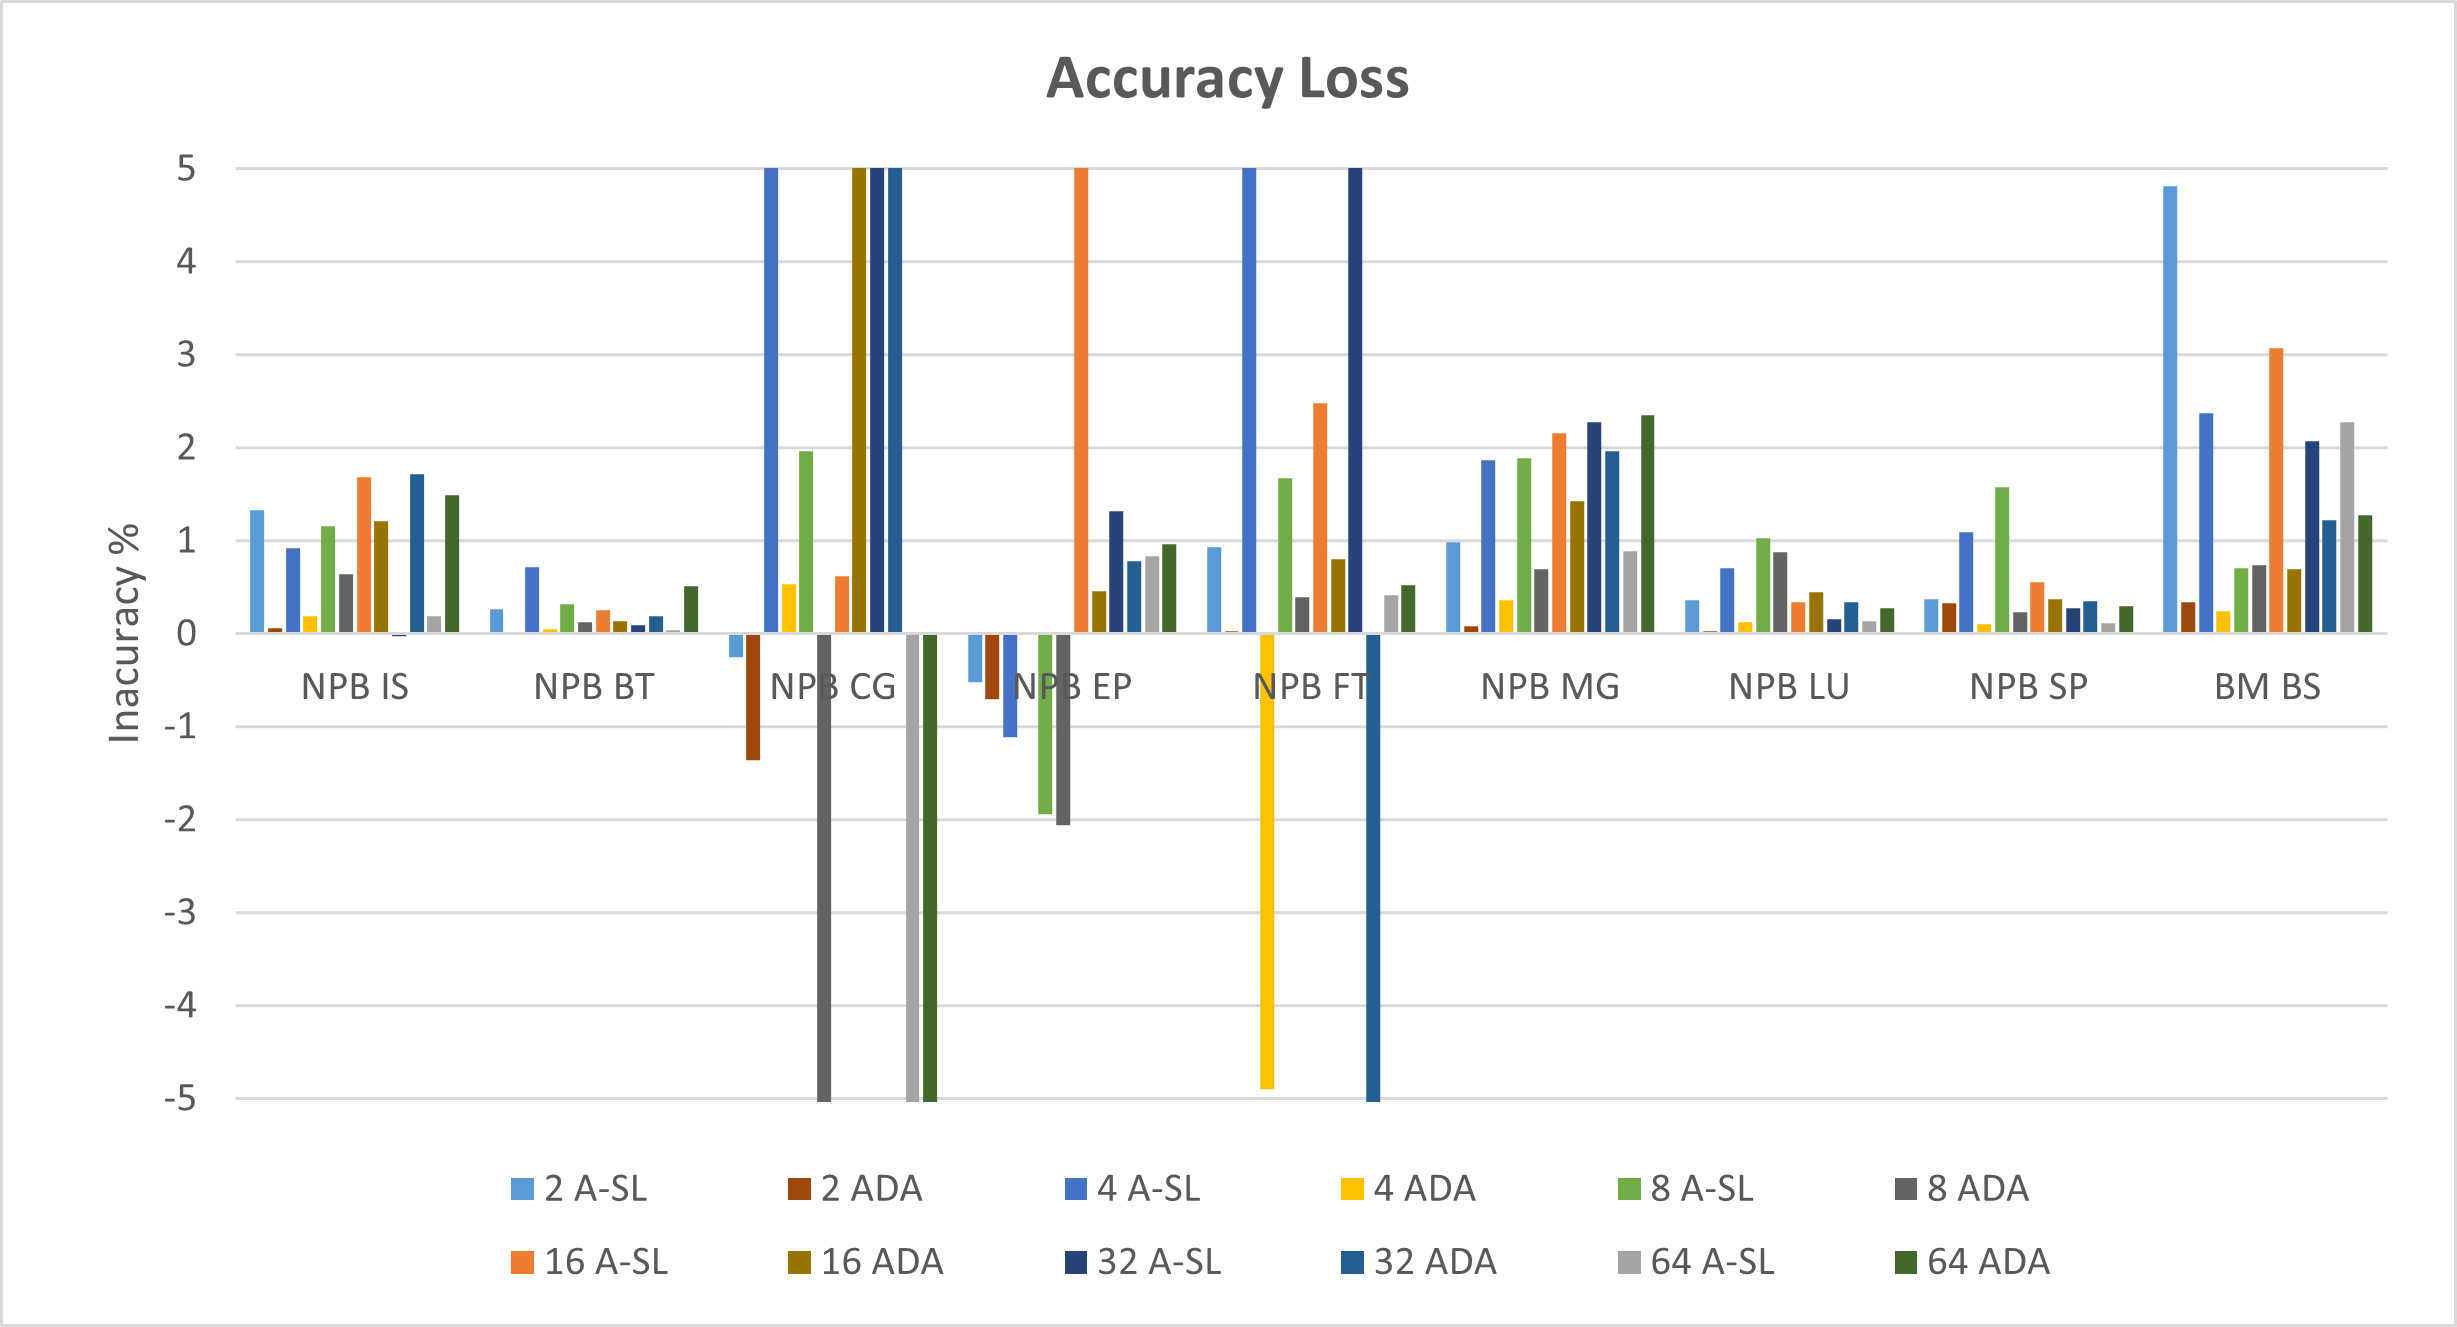
\includegraphics[width=0.8\textwidth]{Images/Accuracy_ADA_INC.png}
    \caption{ Accuracy lost}
    \label{fig:Accuracy_ADAINC}
\end{subfigure}
\begin{subfigure}{\textwidth}
    \centering
    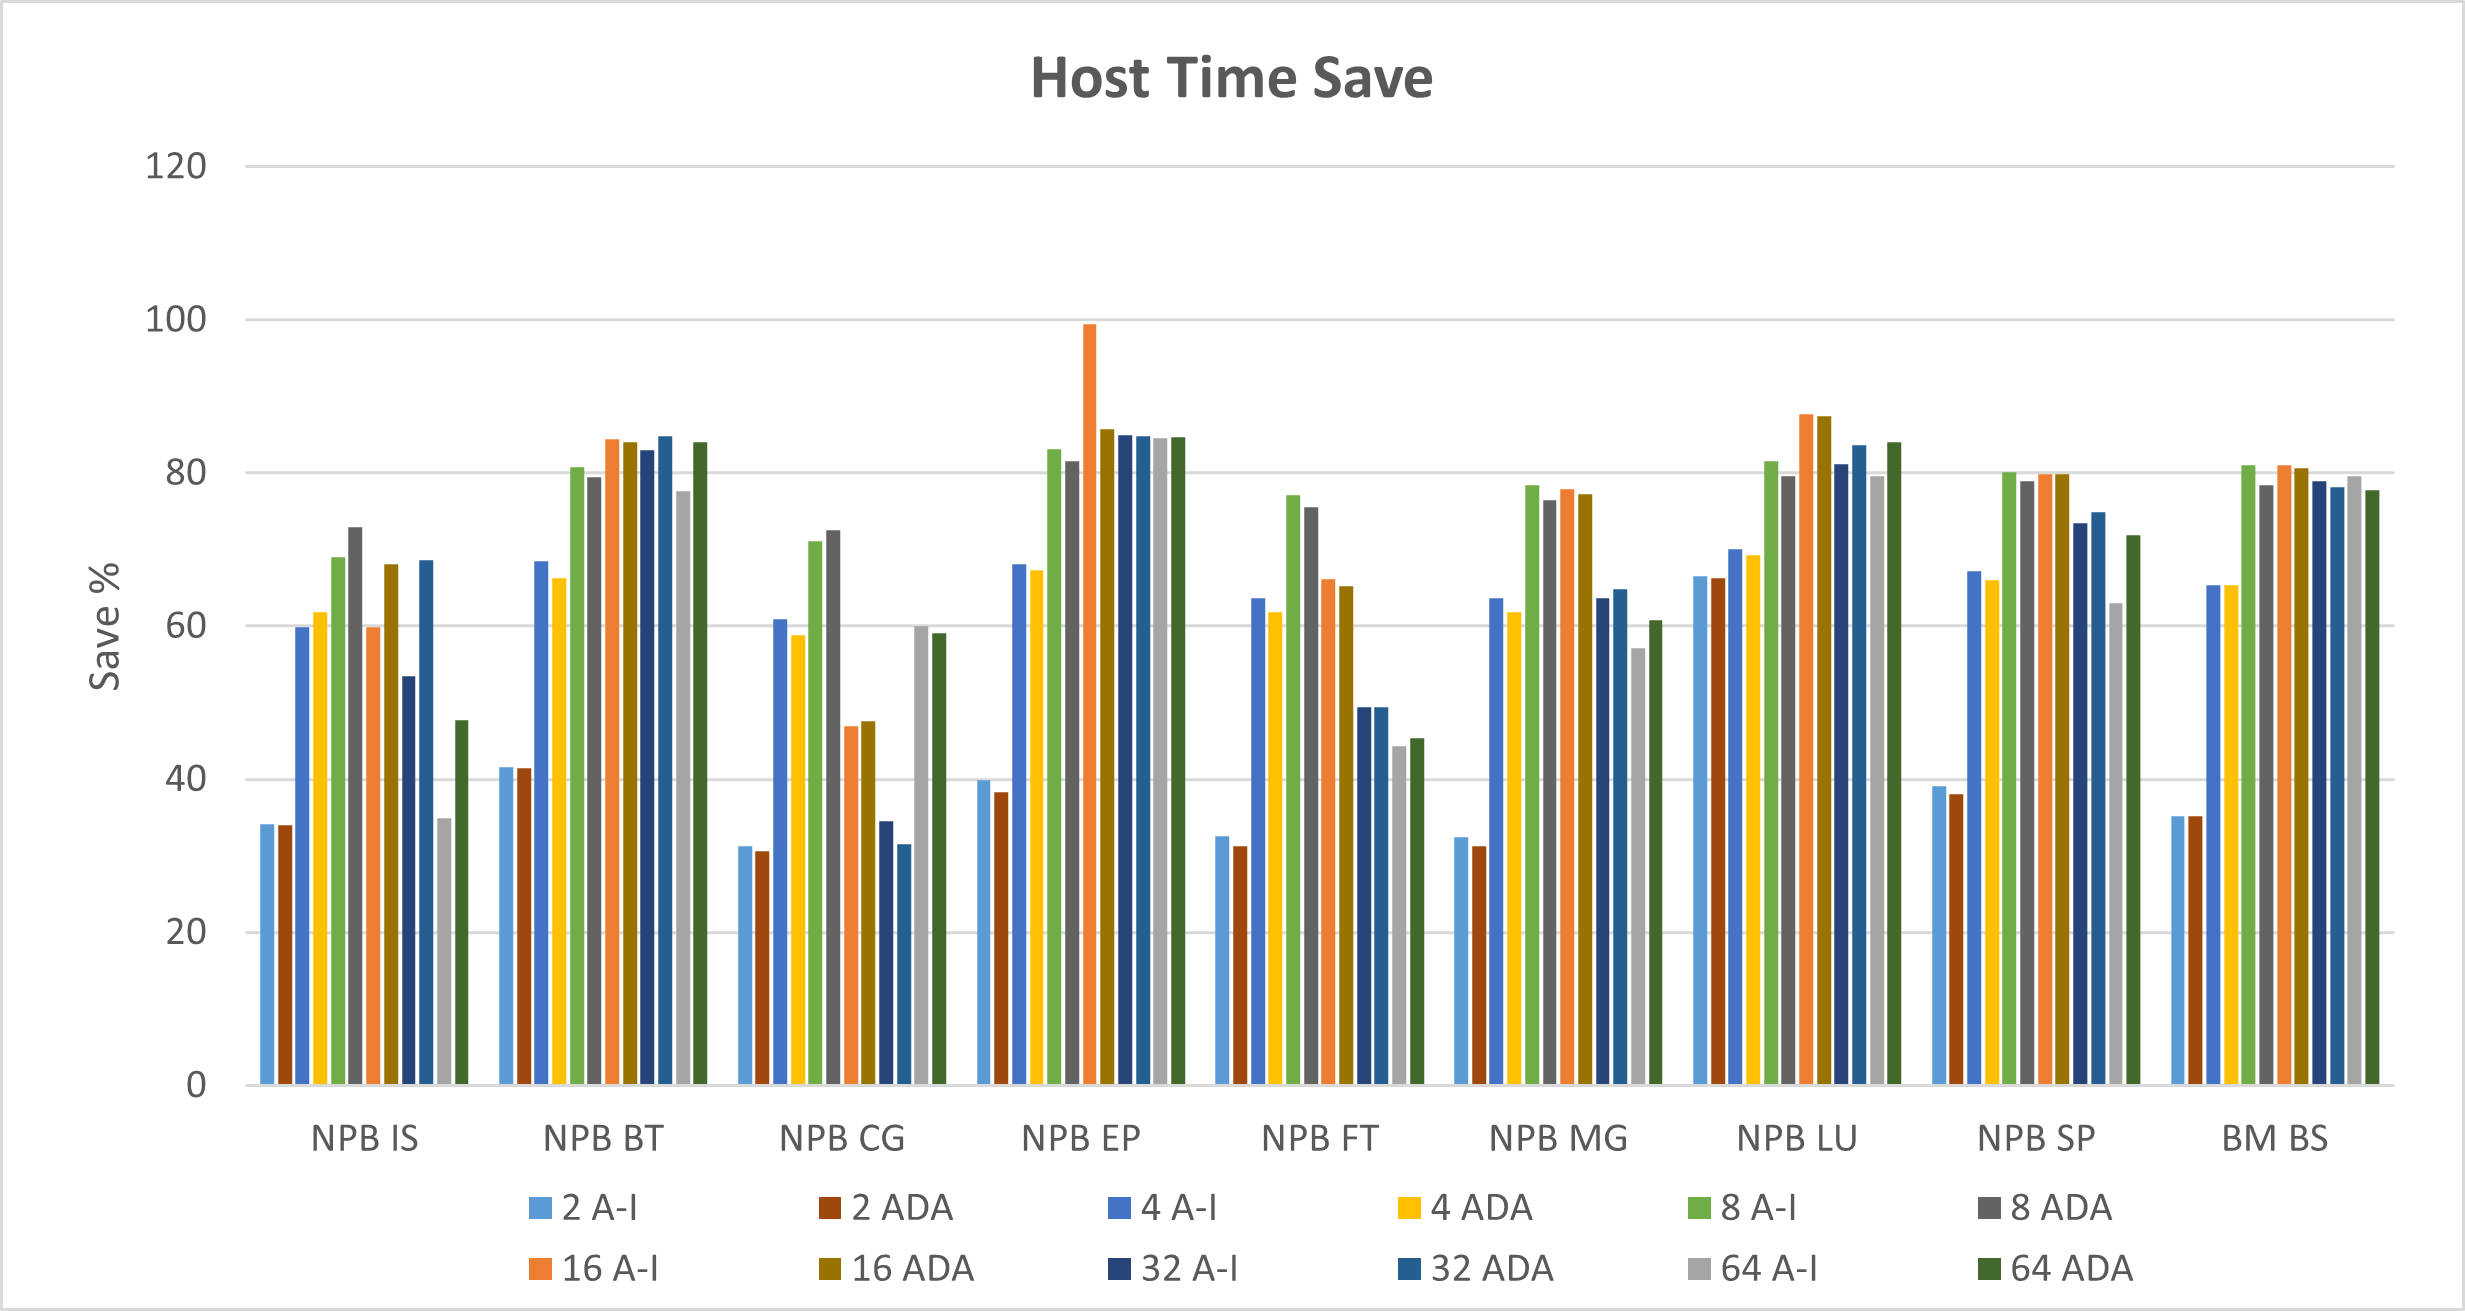
\includegraphics[width=0.8\textwidth]{Images/Host_ADA_INC.png}
    \caption{ Host time save}
    \label{fig:Host_ADAINC}
\end{subfigure}
        
\caption{Dynamic increment results}
\label{fig:results_ADAINC}
\end{figure}

The ADA refers to the first results, while A-SL is related to the new configuration. In general, the dynamic approach with the 
increment value resulted in better performance. Due to the dynamic threshold, when simulating with 32 and 64 cores, there are cases when the
previous approach yielded a better performance. Examples of that are NPB BT, NPB LU, and NPB SP. However, focusing on the remaining cases, 
on average, the performance increment was about 11\%. Additionally, as a consequence of that, the overall host 
time was lower, reducing it by 1\%

Unfortunately, the same did not occur in terms of accuracy. Negative inaccuracy is still present and in all cases, just with a few exceptions, 
there was an accuracy reduction, where, in some cases, such as the NPB FT and NPB EP with sixteen simulated cores, it fell below 95\%. 
Regarding the first topic, the reasons are the same as presented in the previous section. About the other,  
a possible explanation for this could be the nature of the algorithm itself. The adaptive filter may not be designed to 
handle drastic interventions. As shown in \autoref{fig:AF2}, the control action appears to be smooth, even though there are moments, for example, 
in inter-process communications when it should be more aggressive to prevent postponed events in cross-scheduling. The problem was not evident at 
the beginning however, with the dynamic increment, it becomes more notable. 

One of the requirements for this dissertation is to maintain a maximum inaccuracy of 5\% thus, the current approach does not meet this criterion. 
It is crucial to explore alternative methods and optimizations to ensure that the desired level of accuracy is achieved.

\section{Instruction Flow Prediction Algorithm}

As mentioned before, one problem of the previous algorithm is the incapability to reduce the quantum significantly in a short period. A potential 
solution for this issue could involve predicting when this situation is likely to occur. In other words, an attempt can be made to assess when a 
postponed event will take place. If it becomes possible to forecast when such an event will be postponed, adjustments can be made to the quantum 
before it happens. This preemptive action can help prevent significant inaccuracies from occurring. 

Before the simulation initiates, the commands destined for execution are loaded into memory and remain unaltered throughout the simulation. These, 
when executed, can lead to a postponed event. An example of that is the Wait For Event (WFE) instruction, where the \gls{cpu} enters in low-power 
standby state. Furthermore, in general, loops are the backbone of benchmarks, whether due to multiple iterations or the benchmark's inherent 
characteristics, such as testing the transfer of memory blocks between different locations. As a result, the same memory address can be 
encountered more than one time. 

By evaluating the \gls{pc}, it is possible to understand if the processing of one memory address can result in a postponed event (\textit{PPaddr}), 
and so avoid its execution with a large quantum. With this idea in mind, the \gls{ifp} algorithm, as the name suggests, will analyse the \gls{pc} during 
the simulation, in order to perform the prediction of when these will be executed. \autoref{fig_PCAlgorithm} exemplifies an example 
of how the algorithm works.

\begin{figure}[h!]
	\centering
 	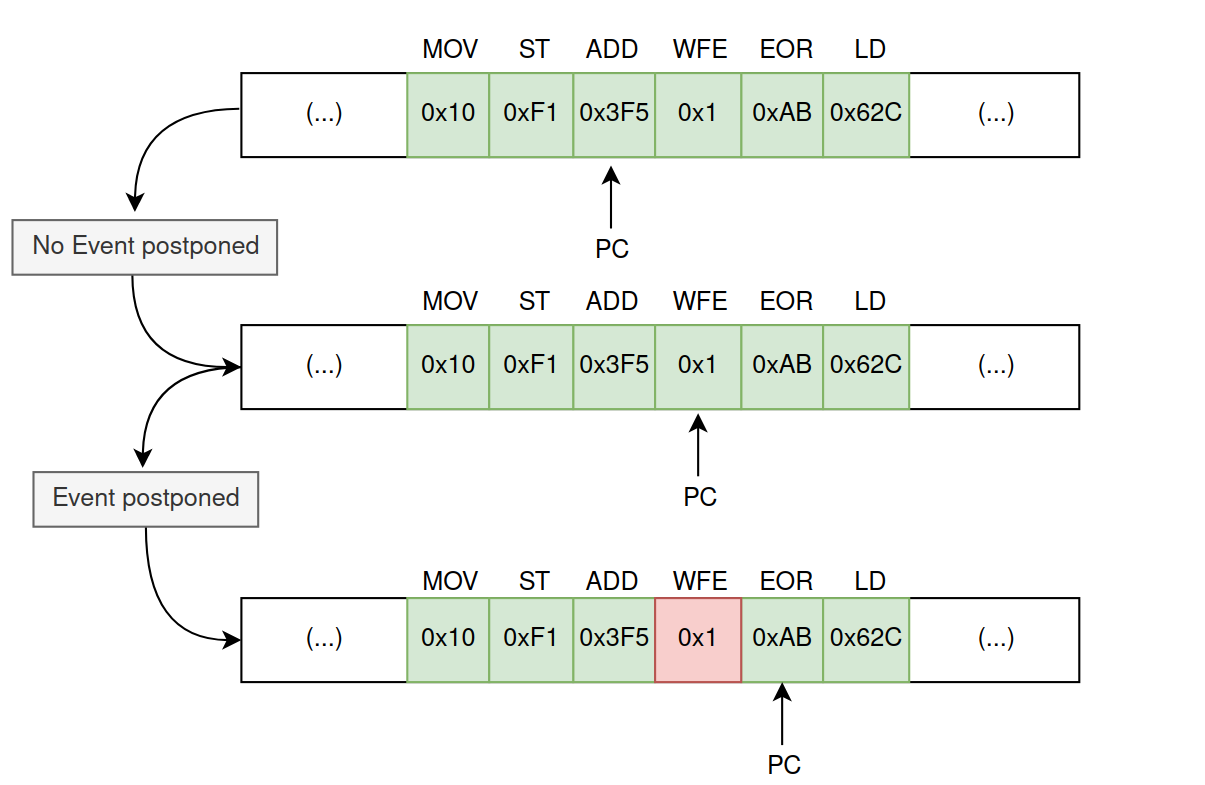
\includegraphics[width=0.7\linewidth]{Images/PCAlgorithm.png}
 	\caption{IFP Algorithm}
	 \label{fig_PCAlgorithm}
\end{figure}

In the beginning, every memory address is considered risk-free, but as the simulation proceeds, it can be changed. When it happens, the processed 
address becomes a spotted address (marked in red in the figure) until the end of the simulation. All these addresses will be taken into 
account in the new quantum calculation, thus to avoid possible noise on the attribution, these will be acknowledged as genuine 
"postponed event generators" only when they are identified regularly.

 
\subsection{Forecast}

Workloads are not straightforward in a way that the \gls{pc} do not follow a linear path. Instructions like "jump" (JMP) or interruptions 
have the potential to redirect the execution flow to different memory locations. Understanding exactly what type of instructions the simulator 
will execute and tracking them is computationally heavy, meaning performance costs. Since the algorithm should be lightweight, it is considered 
that the \gls{pc} is linear, that is, the next \gls{pc} will be the actual plus the instruction width. 

First of all, is used an analytic method to find where the program counter will be in the future. As a result of the previous consideration, 
the \autoref{eq_PCForecast1} was developed.

\begin{equation}
    FPC = PC + \left( \frac{Quantum * InstWidth}{CyclePeriod} \right)
    \label{eq_PCForecast1}
\end{equation}

\begin{equation}
    Quantum = \frac{  \left( FPC - PC \right) * CyclePeriod)}{InstWidth} 
    \label{eq_PCForecast2}
\end{equation}

\hspace*{1cm}

Thereafter, one of two scenarios can unfold, as depicted in the next pictures. Nothing may transpire, if no addresses were 
identified between the \gls{pc} and \gls{fpc}; Alternatively, if the \gls{fpc} corrects its value to the nearest identified 
address, a quantum recalibration is necessary using the \autoref{eq_PCForecast2}. Hence, the synchronization will occur right after the 
execution of the spotted address, avoiding inaccuracy as the cross-schedule event is inserted in the target event queue at the expected time.

\begin{figure} [H]
\centering
\begin{subfigure}{\textwidth}
    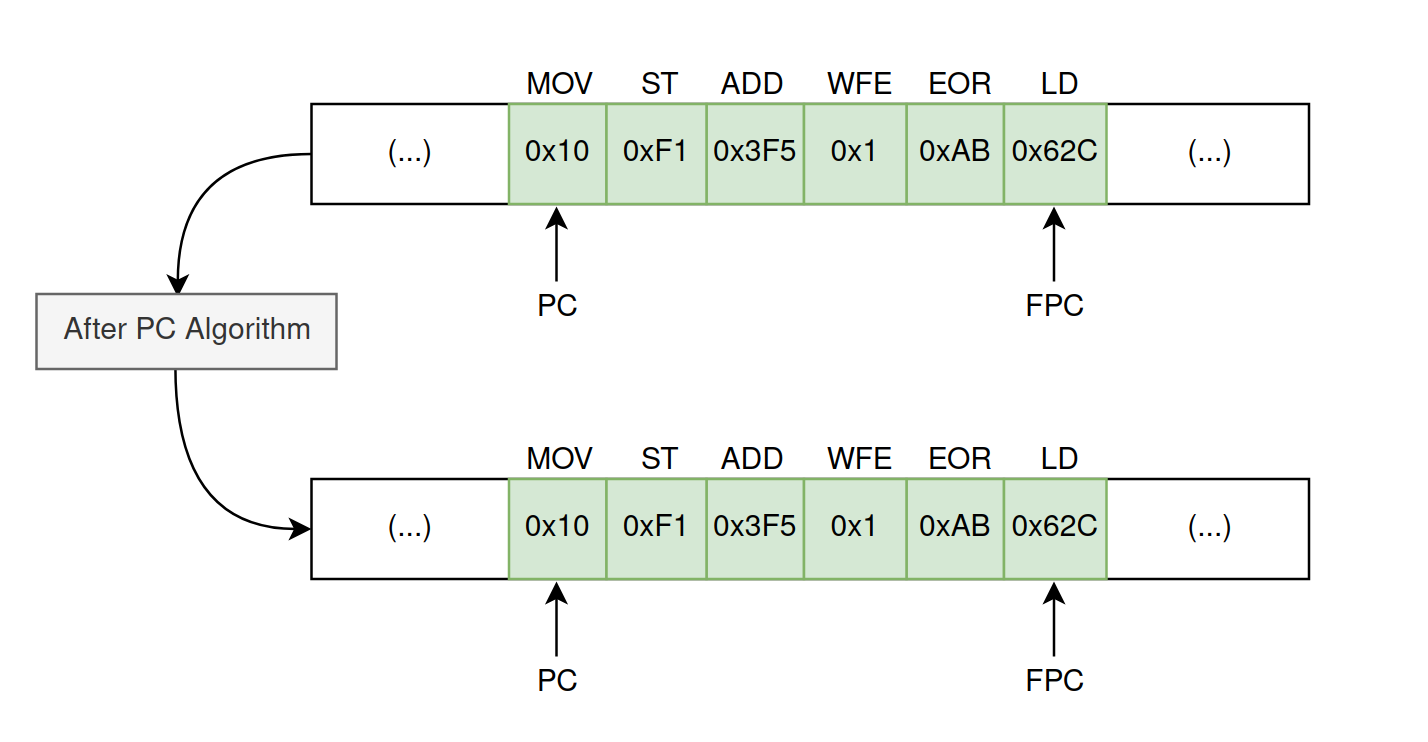
\includegraphics[width=0.8\textwidth]{Images/PCAlgrithm_noCut.png}
    \caption{ Scenario 1 }
    \label{fig:PCAlgrithm_noCut}
\end{subfigure}
\begin{subfigure}{\textwidth}
    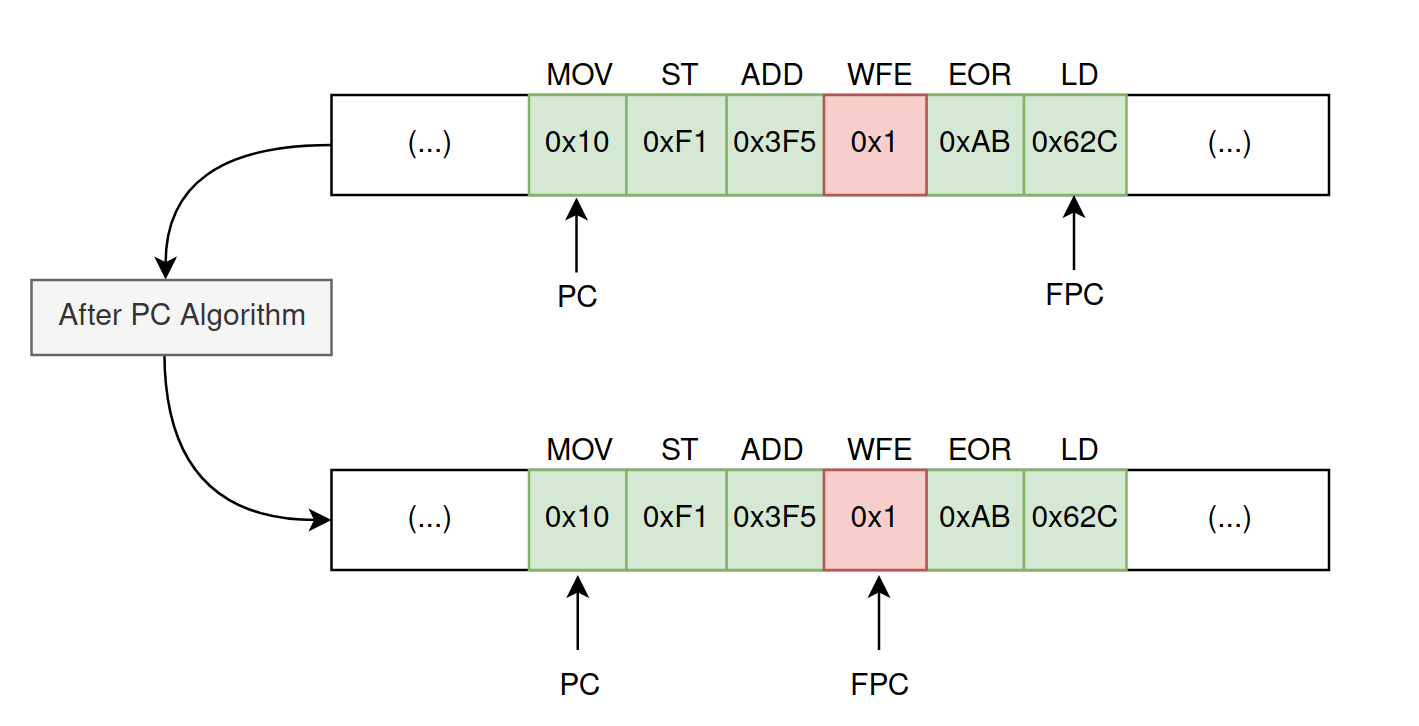
\includegraphics[width=0.8\textwidth]{Images/PCAlgrithm_Cut.png}
    \caption{ Scenario 2 }
    \label{fig:PCAlgrithm_Cut}
\end{subfigure}
        
\caption{Possible scenarios after the forecast}
\label{fig:PCAlgorithm_differentScenarios}
\end{figure}

\subsection{Step Ladder Update}

With the development of this new algorithm, there is a new way to verify if the quantum was reduced, meaning the old one was greater 
than the desirable. For this reason, the Step Ladder algorithm will also verify this situation, counting as an "inaccuracy problem", contributing 
to the reduction of the increment value.

To determine whether the previous scenario occurred, the quantum value before the \gls{ifp} algorithm's action is stored and compared to the current. 
If the stored value is lower than the current quantum, no action is taken. However, if the stored value is equal or higher, it indicates that 
the quantum was reduced, triggering the flag. 


\subsection{Results}

The results of the bare-metal bubble-sort and \glspl{npb} benchmarks execution are presented in the \autoref{fig:results_ADAINCPC}. As previously, 
A-SL refers to the results of the combination of the ADALINE-based and Step Ladder algorithms, and IFP points to the 
\gls{ifp} algorithm intervention results.

As expected, there was a drop in the performance gain when compared to the previous. This was about 5\%, which in practice, 
reflected in an increment of the host time of around 0.3\%. Nevertheless, there are a few cases in the algorithm's action 
conducted into better performance, for instance, the NPB BT over two and eight simulated cores. 

The most distinguished side is the accuracy, where the \gls{pc} analysis inclusion allowed the removal of the inaccuracy peaks that existed 
in the A-SL version hence, the previously mentioned cases that passed the 5\% are now within the limit. Only the NPB FT with 32
and NPB CG with 64 simulated cores are exceptions however, these should not be considered, as explained further in this chapter. 
When considering up to 16 simulated cores, there was approximately an increment 
of about 0.5\% in accuracy. 

Negative inaccuracy persists in the simulations. While the occurrence of this issue has been reduced in comparison to the initial version, 
it is important to retain that this problem remains associated with par-gem5, as aforementioned. 

It can be concluded the \gls{ifp} algorithm presence allowed the quantum to immediately reduce its value. It also can be identified when 
analysing the worst-case scenario of inaccuracy, where drops can reach up to 10\%. The tradeoff was even improved since 
the enhancements in accuracy outweighed the increase in host time.

\begin{figure}[H]
\centering
\begin{subfigure}{\textwidth}
    \centering
    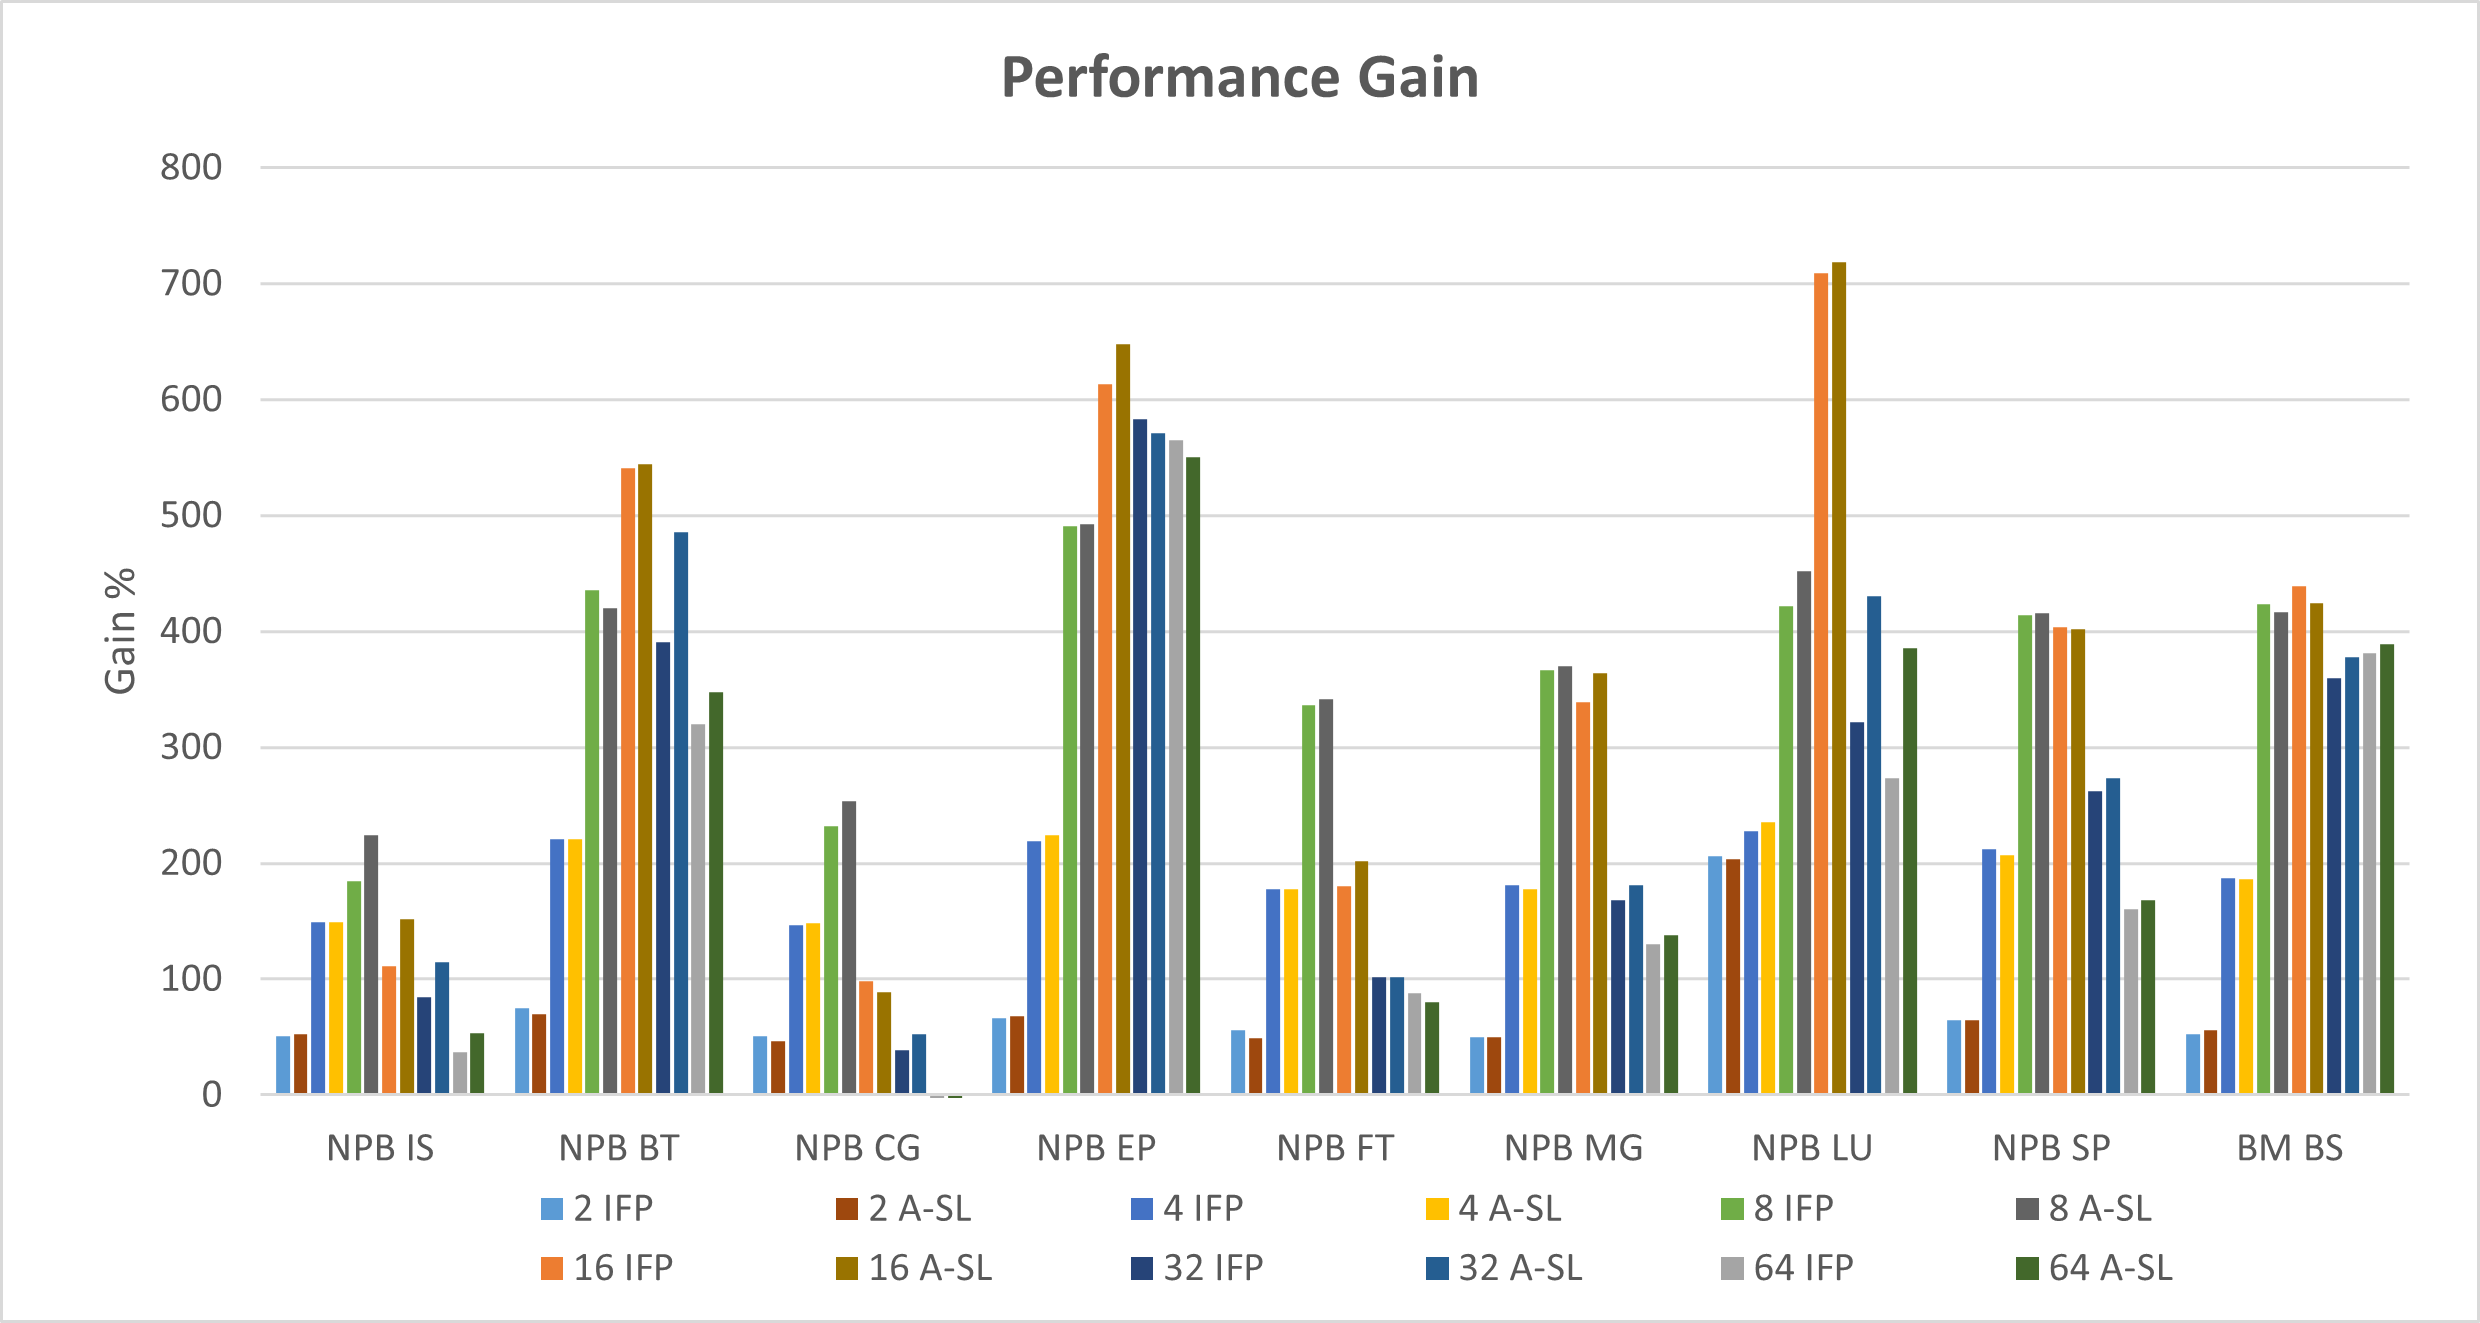
\includegraphics[width=0.8\textwidth]{Images/Performance_ADA_INC_PC.png}
    \caption{ Performance gain}
    \label{fig:Performance_ADAINCPC}
\end{subfigure}
\begin{subfigure}{\textwidth}
    \centering
    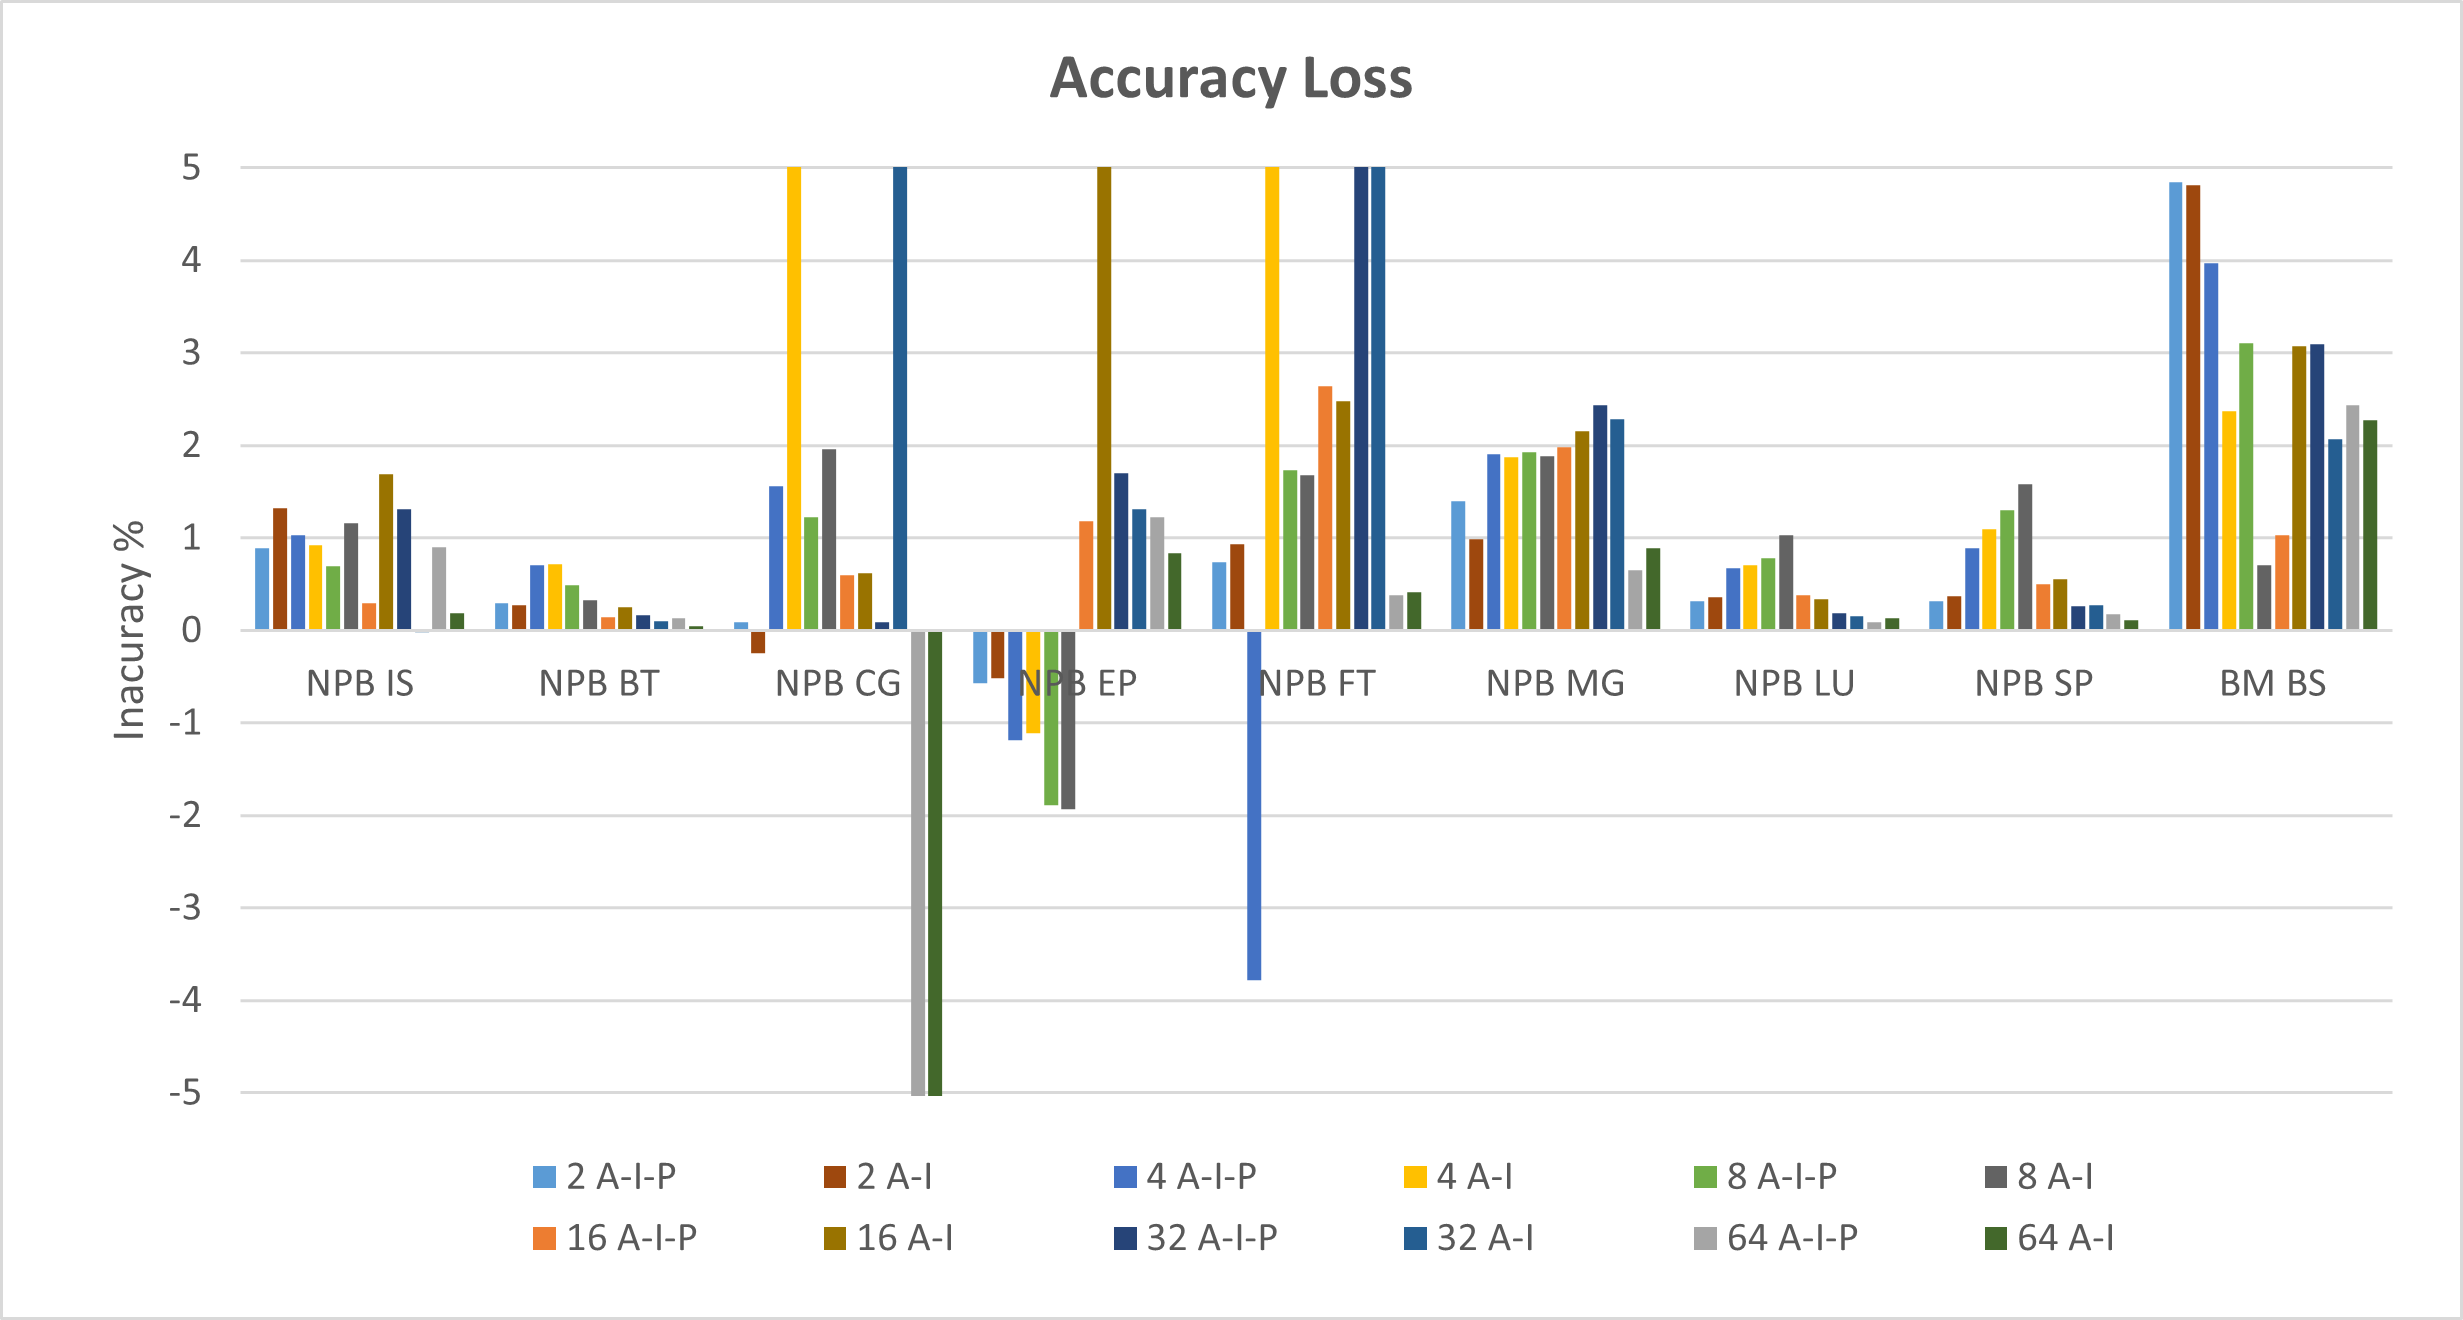
\includegraphics[width=0.8\textwidth]{Images/Accuracy_ADA_INC_PC.png}
    \caption{ Accuracy lost}
    \label{fig:Accuracy_ADAINCPC}
\end{subfigure}
\begin{subfigure}{\textwidth}
    \centering
    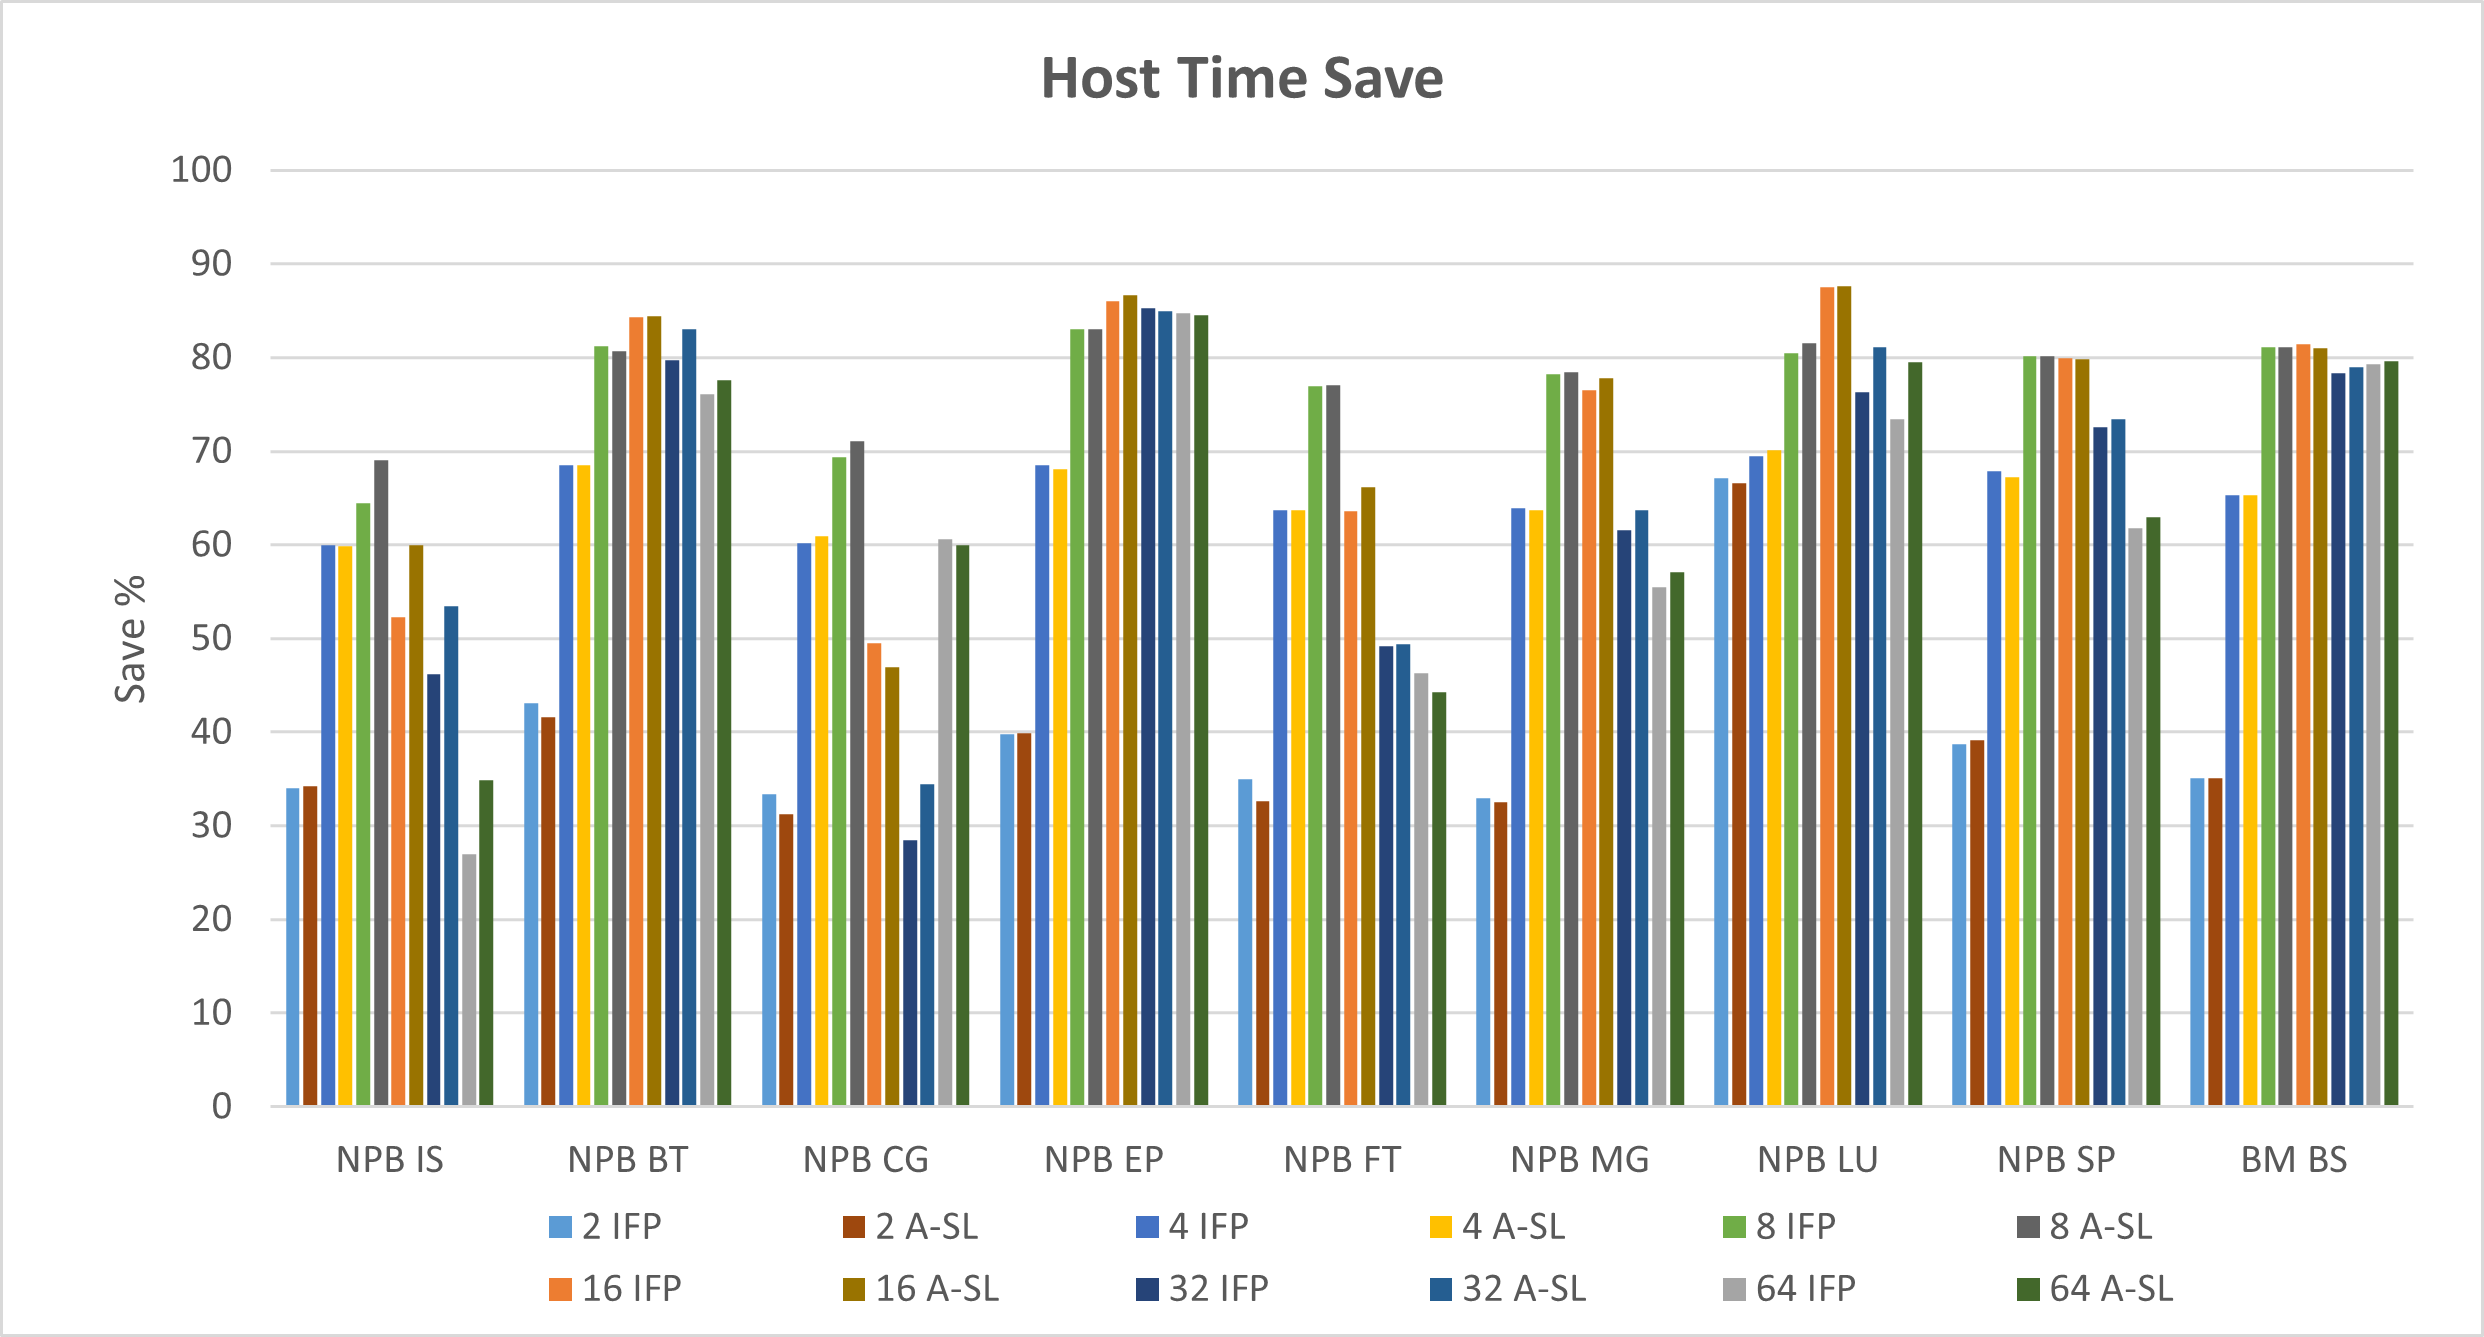
\includegraphics[width=0.8\textwidth]{Images/Host_ADA_INC_PC.png}
    \caption{ Host time save}
    \label{fig:Host_ADAINCPC}
\end{subfigure}
        
\caption{IFP algorithm results}
\label{fig:results_ADAINCPC}
\end{figure}


\section{Loop Detection Algorithm}

As mentioned earlier in this chapter, loops are strongly present in benchmarks. Thinking in this perspective, if a record of every executed 
memory address is made, a loop can be identified in real-time. Combining this with the previous algorithms, the quantum could be adapted in a way 
to have the highest value possible. Furthermore, the accuracy would be nearly perfect since all cross-schedule events would be known, allowing 
for precise adaptation. The later figure presents how this idea can be integrated into the quantum calculation.


\begin{figure}[h!]
	\centering
 	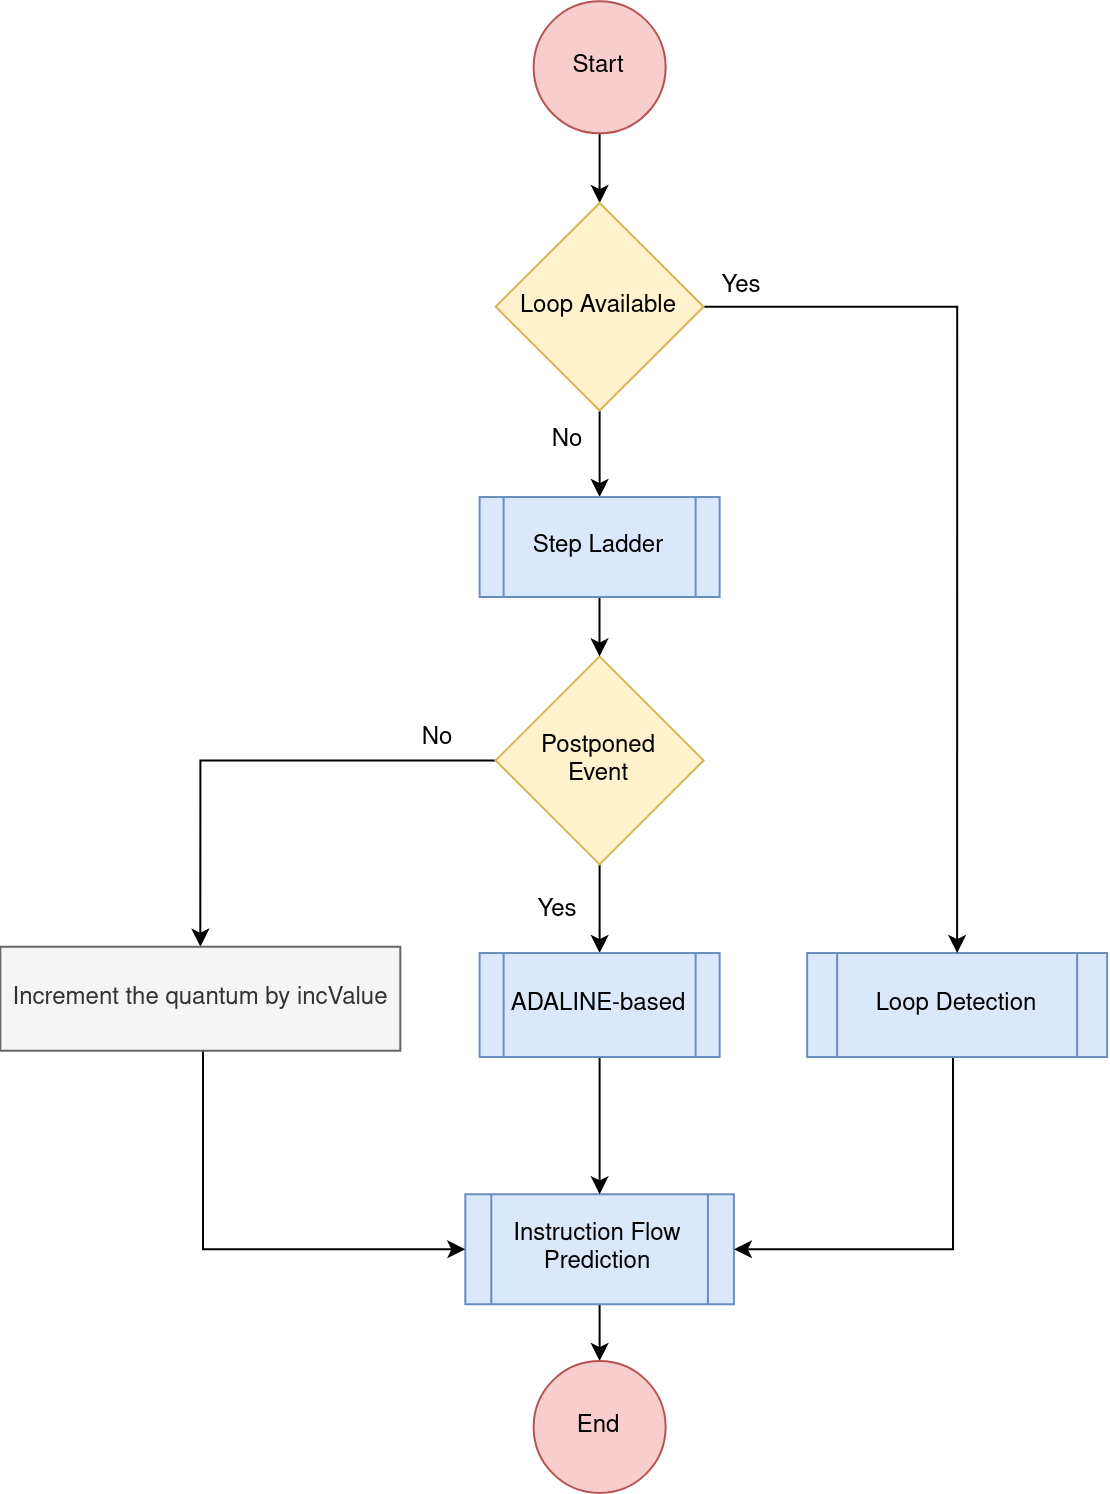
\includegraphics[width=0.55\linewidth]{Images/ADA_and_REP.png}
 	\caption{Quantum definition with Loop Detection algorithm}
	 \label{fig_ADA_and_REP}
\end{figure}


When the simulation starts, there is no information about loops or \textit{PPaddrs}. To achieve this, it would be necessary to execute the simulation 
once and then obtain the results, which do not meet the requirements. One solution is to conduct the simulation in a regular manner while 
simultaneously recording the executed memory addresses. When a loop is detected, the algorithm begins utilizing the loop to calculate the quantum 
until the \gls{pc} no longer follows the loop's path. At that point, the loop is reset, and the process starts anew.

\subsection{Hare-Tortoise Algorithm}

The detection method must be light otherwise, the simulation performance is set in danger. One algorithm with this characteristic is Floyd's 
Tortoise and Hare. It consists of two pointers, one twice faster than the other. If both match at some point, means that there is a 
loop, as shown in the figure below.

\begin{figure}[H]
	\centering
 	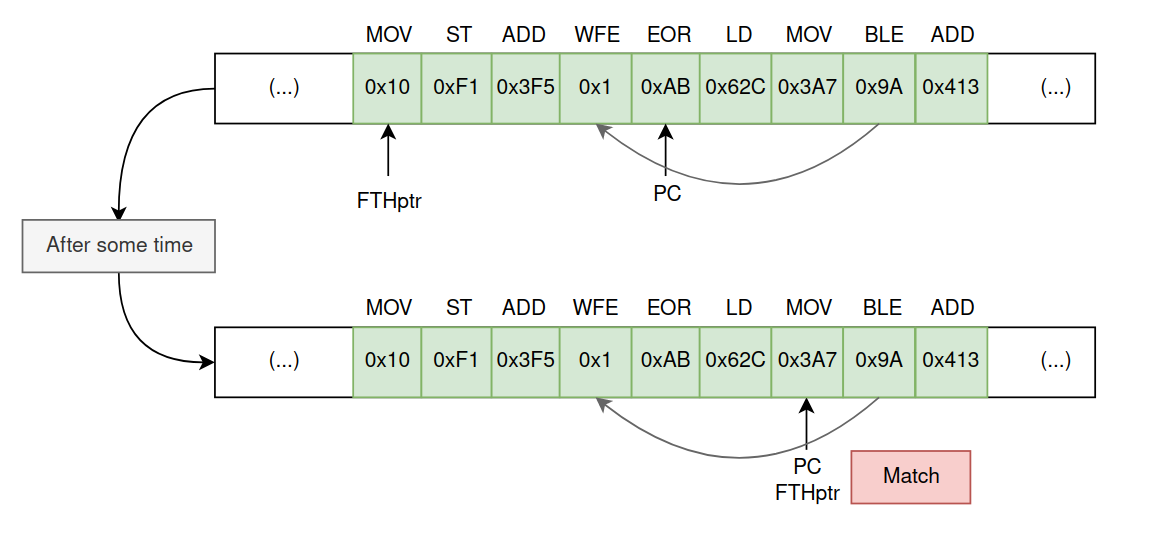
\includegraphics[width=0.8\linewidth]{Images/FTH_algorithm.png}
 	\caption{Hare-Tortoise Algorithm}
	 \label{fig_FTH_algorithm}
\end{figure}

The flowchart present in the \autoref{fig_Repetition_flowchart} describes the Loop Detection flow. 
In this case, the faster pointer is the \gls{pc}, and the slower one is the FTHptr. A match occurs when both are pointing to the same memory at 
the same time. Going into the process in detail, loop delineation can be achieved through two methods. Firstly, an analysis can be conducted on 
the preceding memory address to precisely define the loop boundaries. Alternatively, after the initial match, the FTHptr remains in the same position 
while the \gls{pc} continues execution. When they match once more, the loop becomes well-defined. In terms of performance, it is trivial the 
second approach is more underweight, reason why it was chosen. After the detection, it is necessary to keep track of the \gls{pc}, as mentioned 
earlier. It is done by comparing the actual \gls{pc} with the expected one. If they match, no action is taken. In the opposite way, if there 
is a mismatch, the loop is discarded and the entire detection process starts again.

\begin{figure}[h!]
	\centering
 	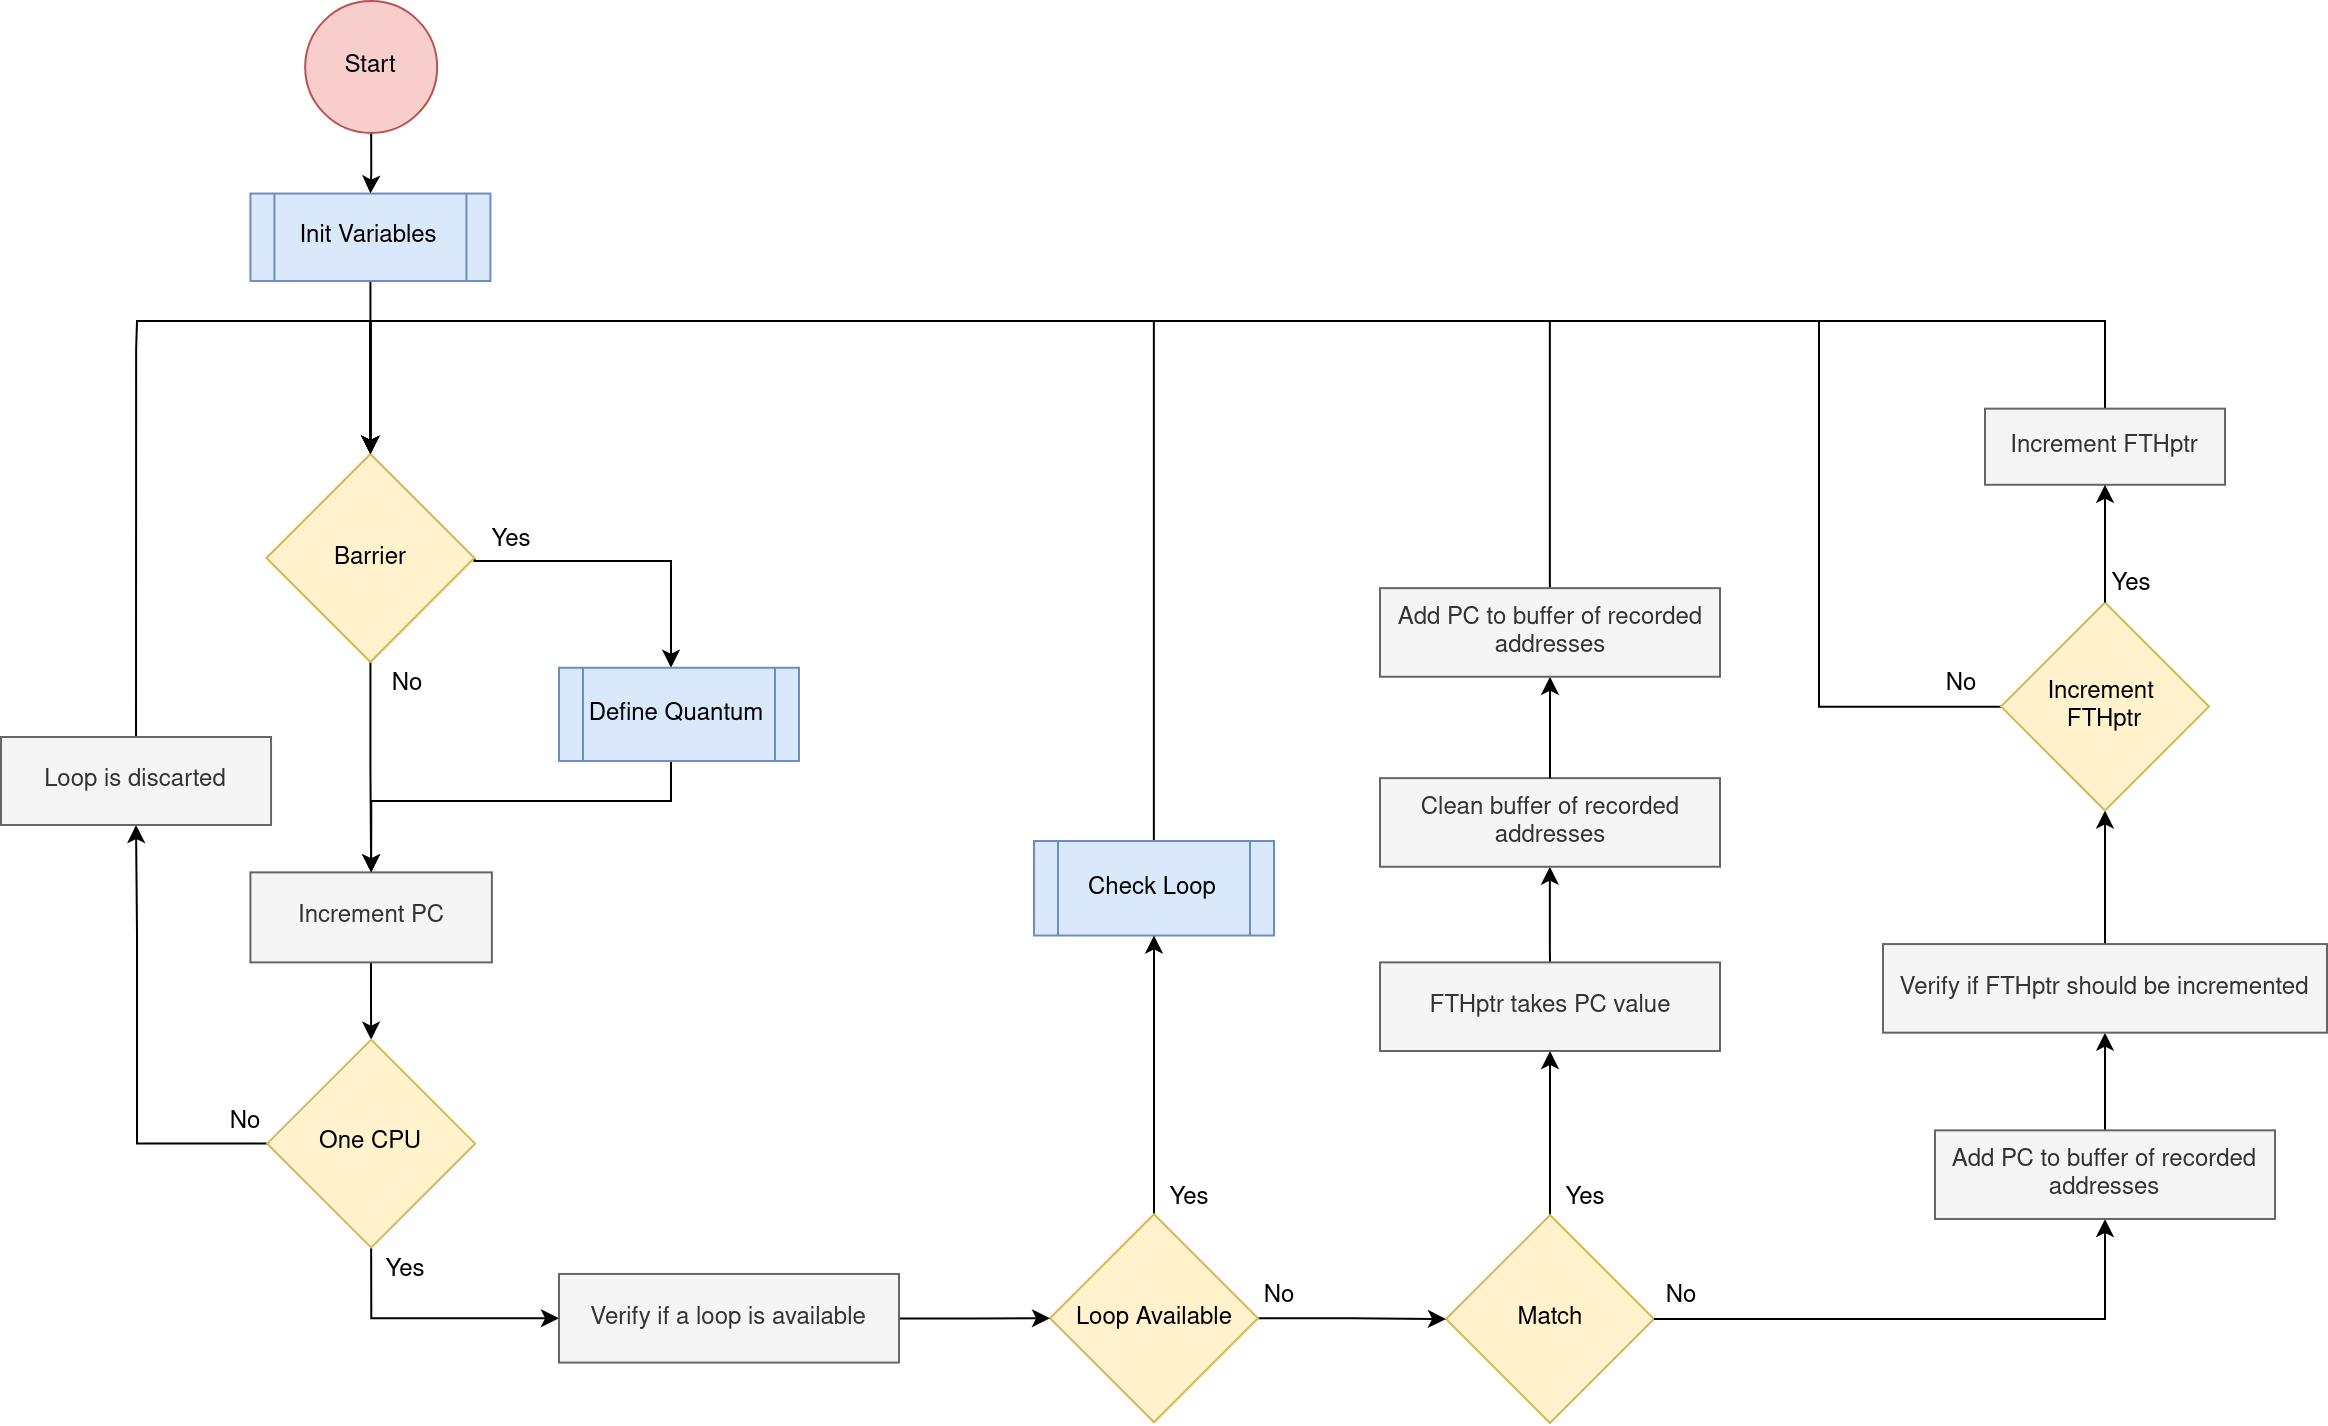
\includegraphics[width=0.9\linewidth]{Images/Repetition_flowchart.png}
 	\caption{Loop Detection flowchart}
	 \label{fig_Repetition_flowchart}
\end{figure}


Although this technique is simple and very effective, it has some inherent problems. The first issue pertains to the inability to detect 
nested loops. Another challenge is the incapability to identify subsequent loops following the one that has been detected. Lastly, the most crucial 
problem is the difficulty in detecting conditions within loops. All of these can be solved with the \gls{pc} track nevertheless, this solution 
may cut the benefits of the algorithm, since these problems can be recurrent in the benchmark. 

Another problem is the multi-thread environment. When more than one \gls{cpu} is active, the \gls{pc} is used by multiple event queues, 
meaning an unpredictable pointer. In this situation is almost impossible to identify any loop, thus a a restriction that permits the Loop 
Detection only when one \gls{cpu} is active was implemented.   
If there is a loop defined and the other \glspl{cpu} wakes up, this is automatically discarded, and the algorithm 
stops, restarting again when the later condition reverts. 

\subsection{Quantum Calculation}

The quantum calculation is done at the synchronization point, as shown in detail in the \autoref{fig_Repetition_flowchart_quantum}. 
It can be divided into 2 distinct tasks. The first one is to classify the loop addresses. The second is the calculation of the new quantum. 

Regarding the primary task, it is only executed when the loop is new, so it is only done once per loop. The loop's size is utilized to 
determine whether it is the same loop or not. This approach is chosen for its simplicity and the low probability of encountering two different 
loops with identical sizes. After this verification, an iteration within the loop is made, comparing these with the spotted addresses. If there 
is a match, that value is associated with a \textit{PPaddr}. 

\begin{figure}[H]
	\centering
 	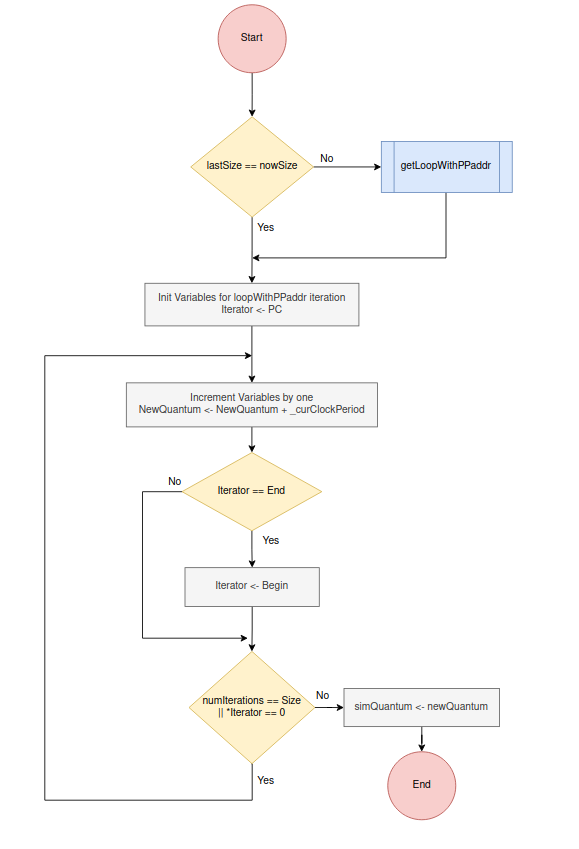
\includegraphics[width=0.5\linewidth]{Images/Repetition_flowchart_quantum.png}
 	\caption{Quantum calculation flowchart}
	 \label{fig_Repetition_flowchart_quantum}
\end{figure}

To calculate the quantum, the last task uses an iteration technique, as demonstrated in the flowchart. 
The iterator starts where the \gls{pc} is, and pursues the loop until it either finds a \textit{PPaddr} or reaches the starting point. 
The quantum starts with the minimum value, which is the clock period, and increments that value in each iteration.

\subsection{Results}

\autoref{fig:results_ADAINCPCREP} exhibits the results of the executed benchmarks with the previous (IFP) and new (LD) configurations. 
When compared with the previous algorithm, the new one does not bring a better tradeoff between performance and accuracy. 
In reality, it is the opposite, that is, the Loop Detection action resulted in a loss of benefits. 


\begin{figure}[H]
\centering
\begin{subfigure}{\textwidth}
    \centering
    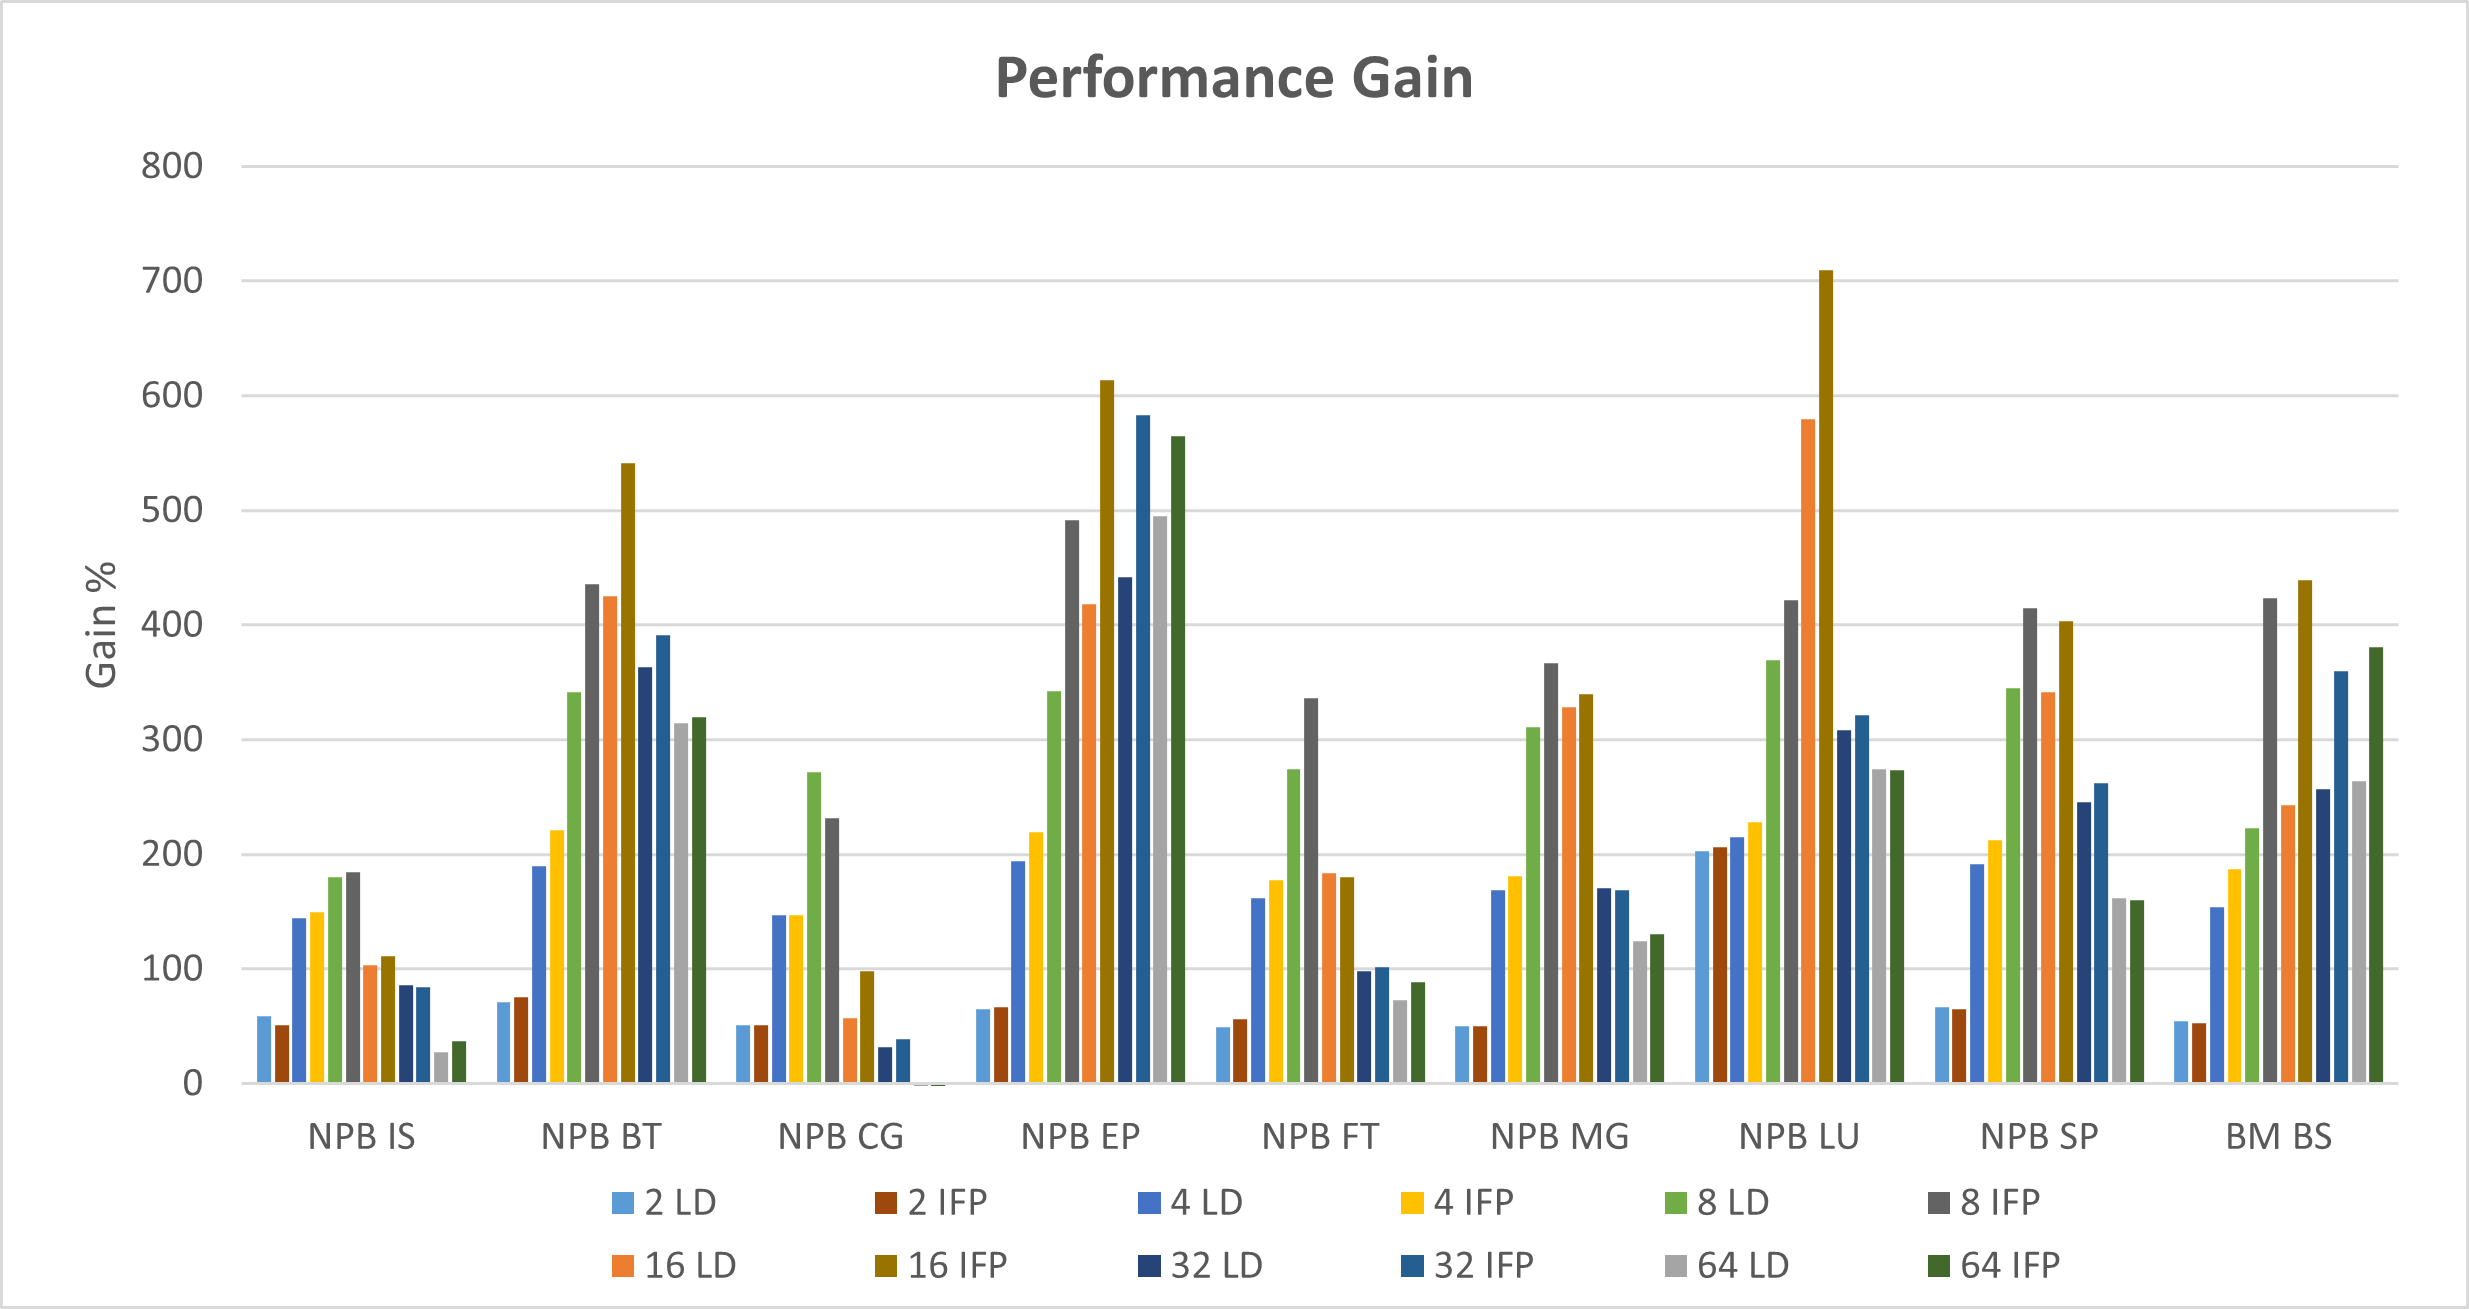
\includegraphics[width=0.8\textwidth]{Images/Performance_REP.png}
    \caption{ Performance gain}
    \label{fig:Performance_ADAINCPCREP}
\end{subfigure}
\begin{subfigure}{\textwidth}
    \centering
    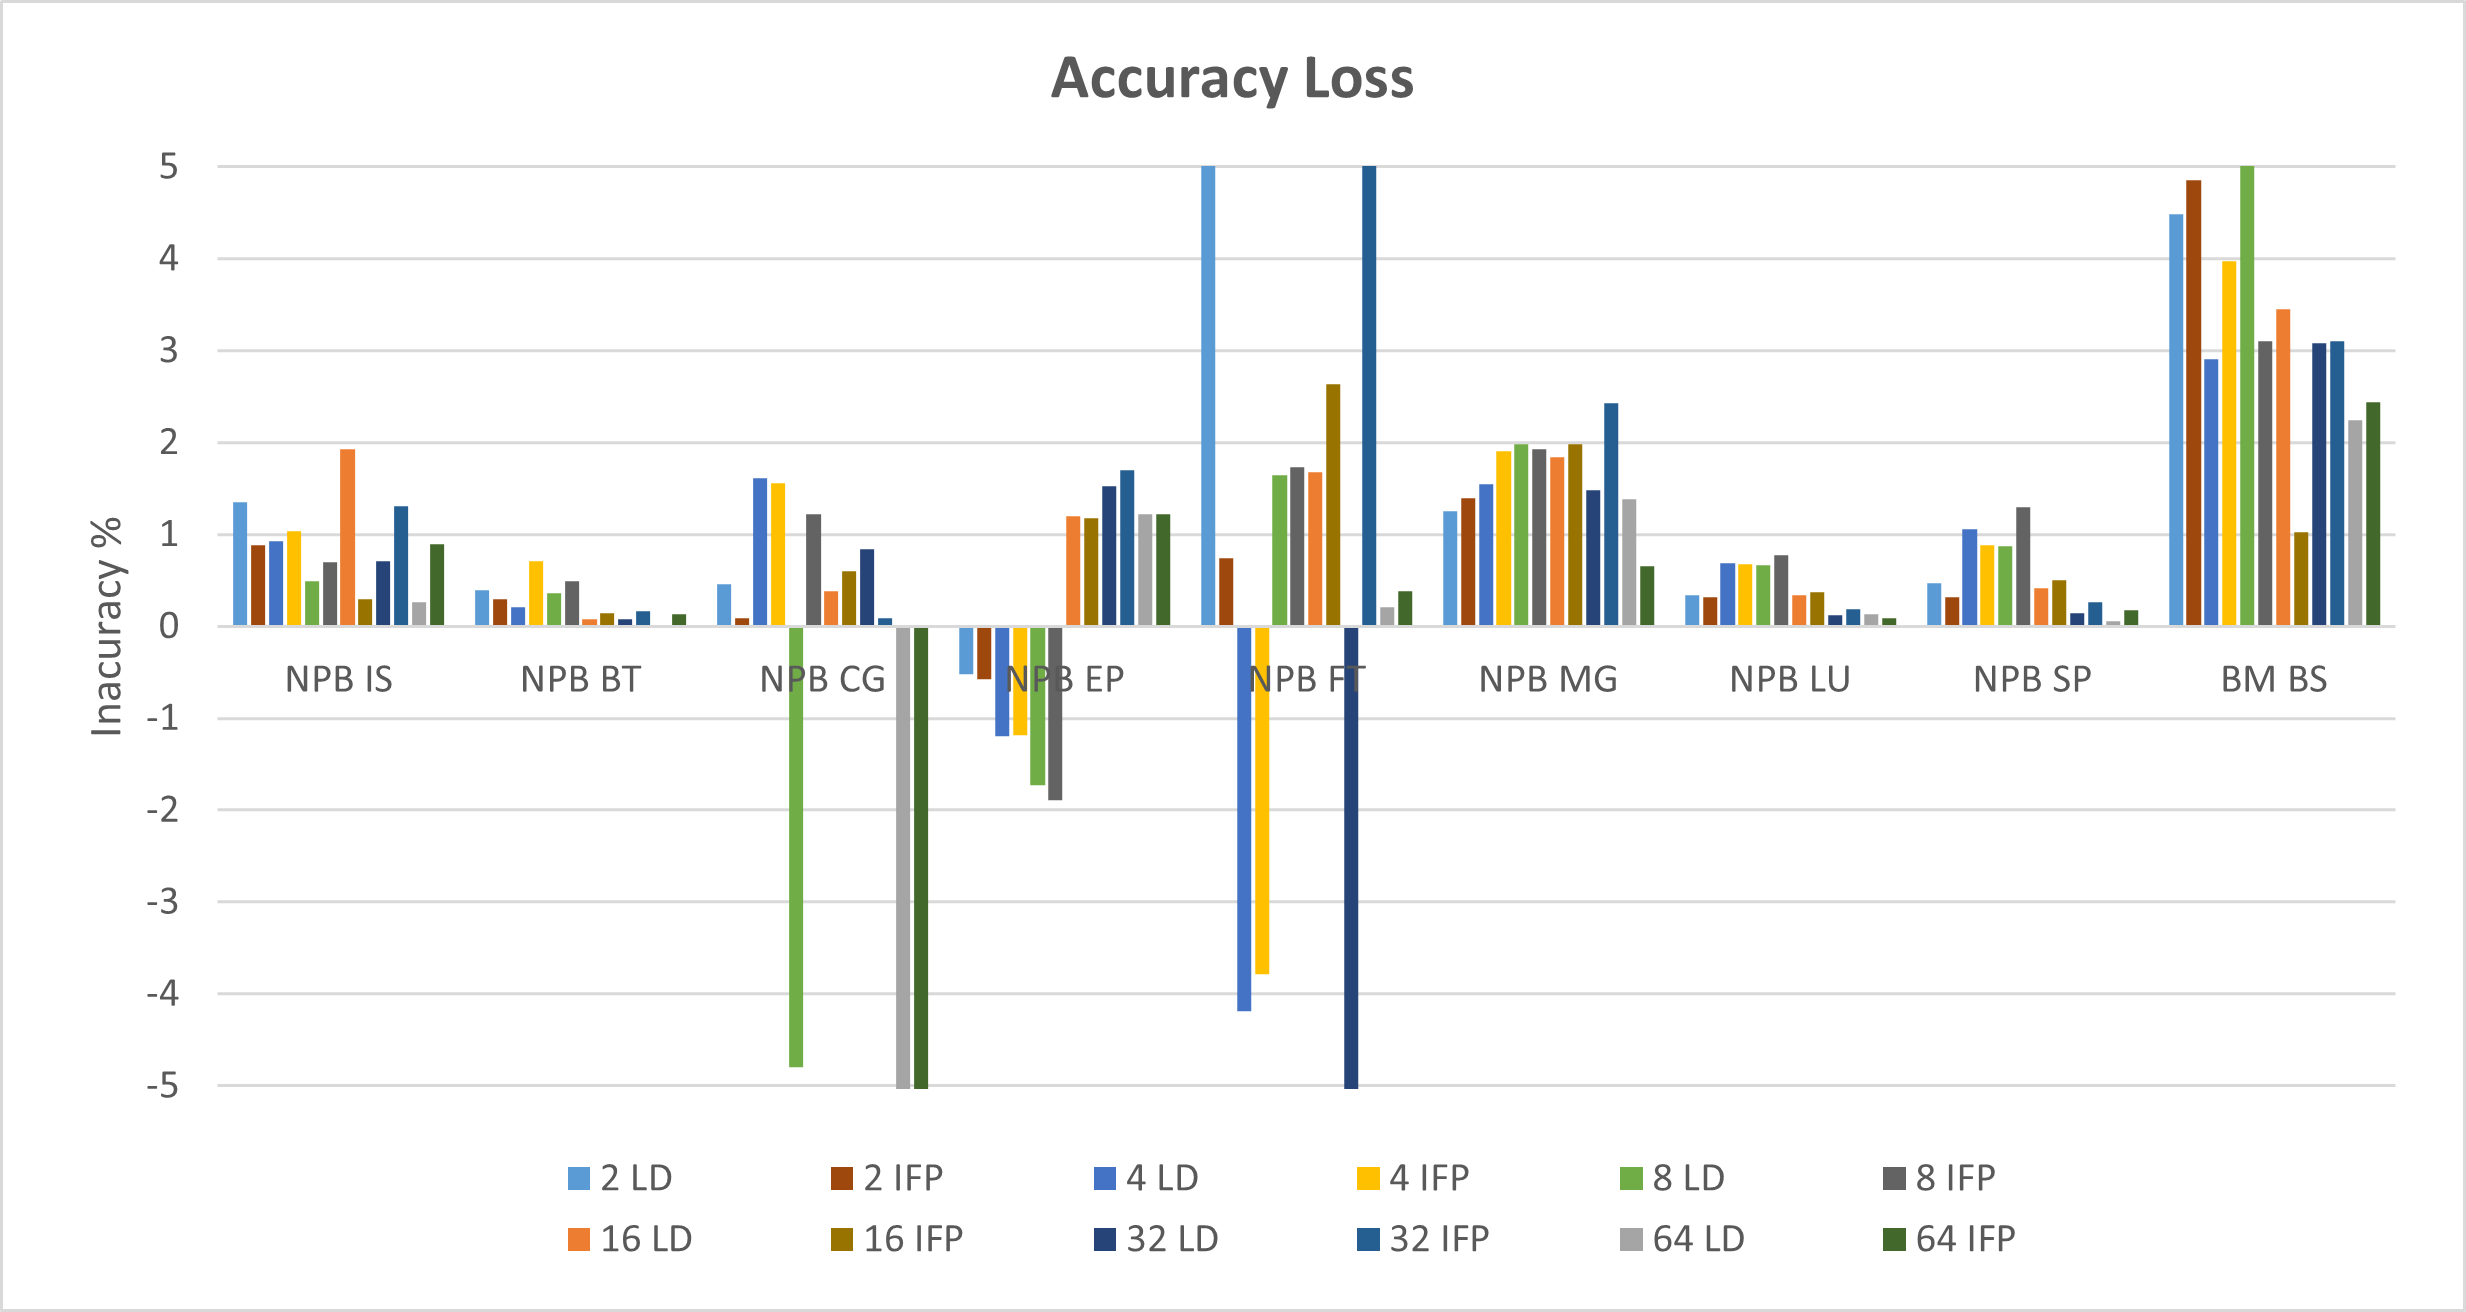
\includegraphics[width=0.8\textwidth]{Images/Accuracy_REP.png}
    \caption{ Accuracy lost}
    \label{fig:Accuracy_ADAINCPCREP}
\end{subfigure}
\begin{subfigure}{\textwidth}
    \centering
    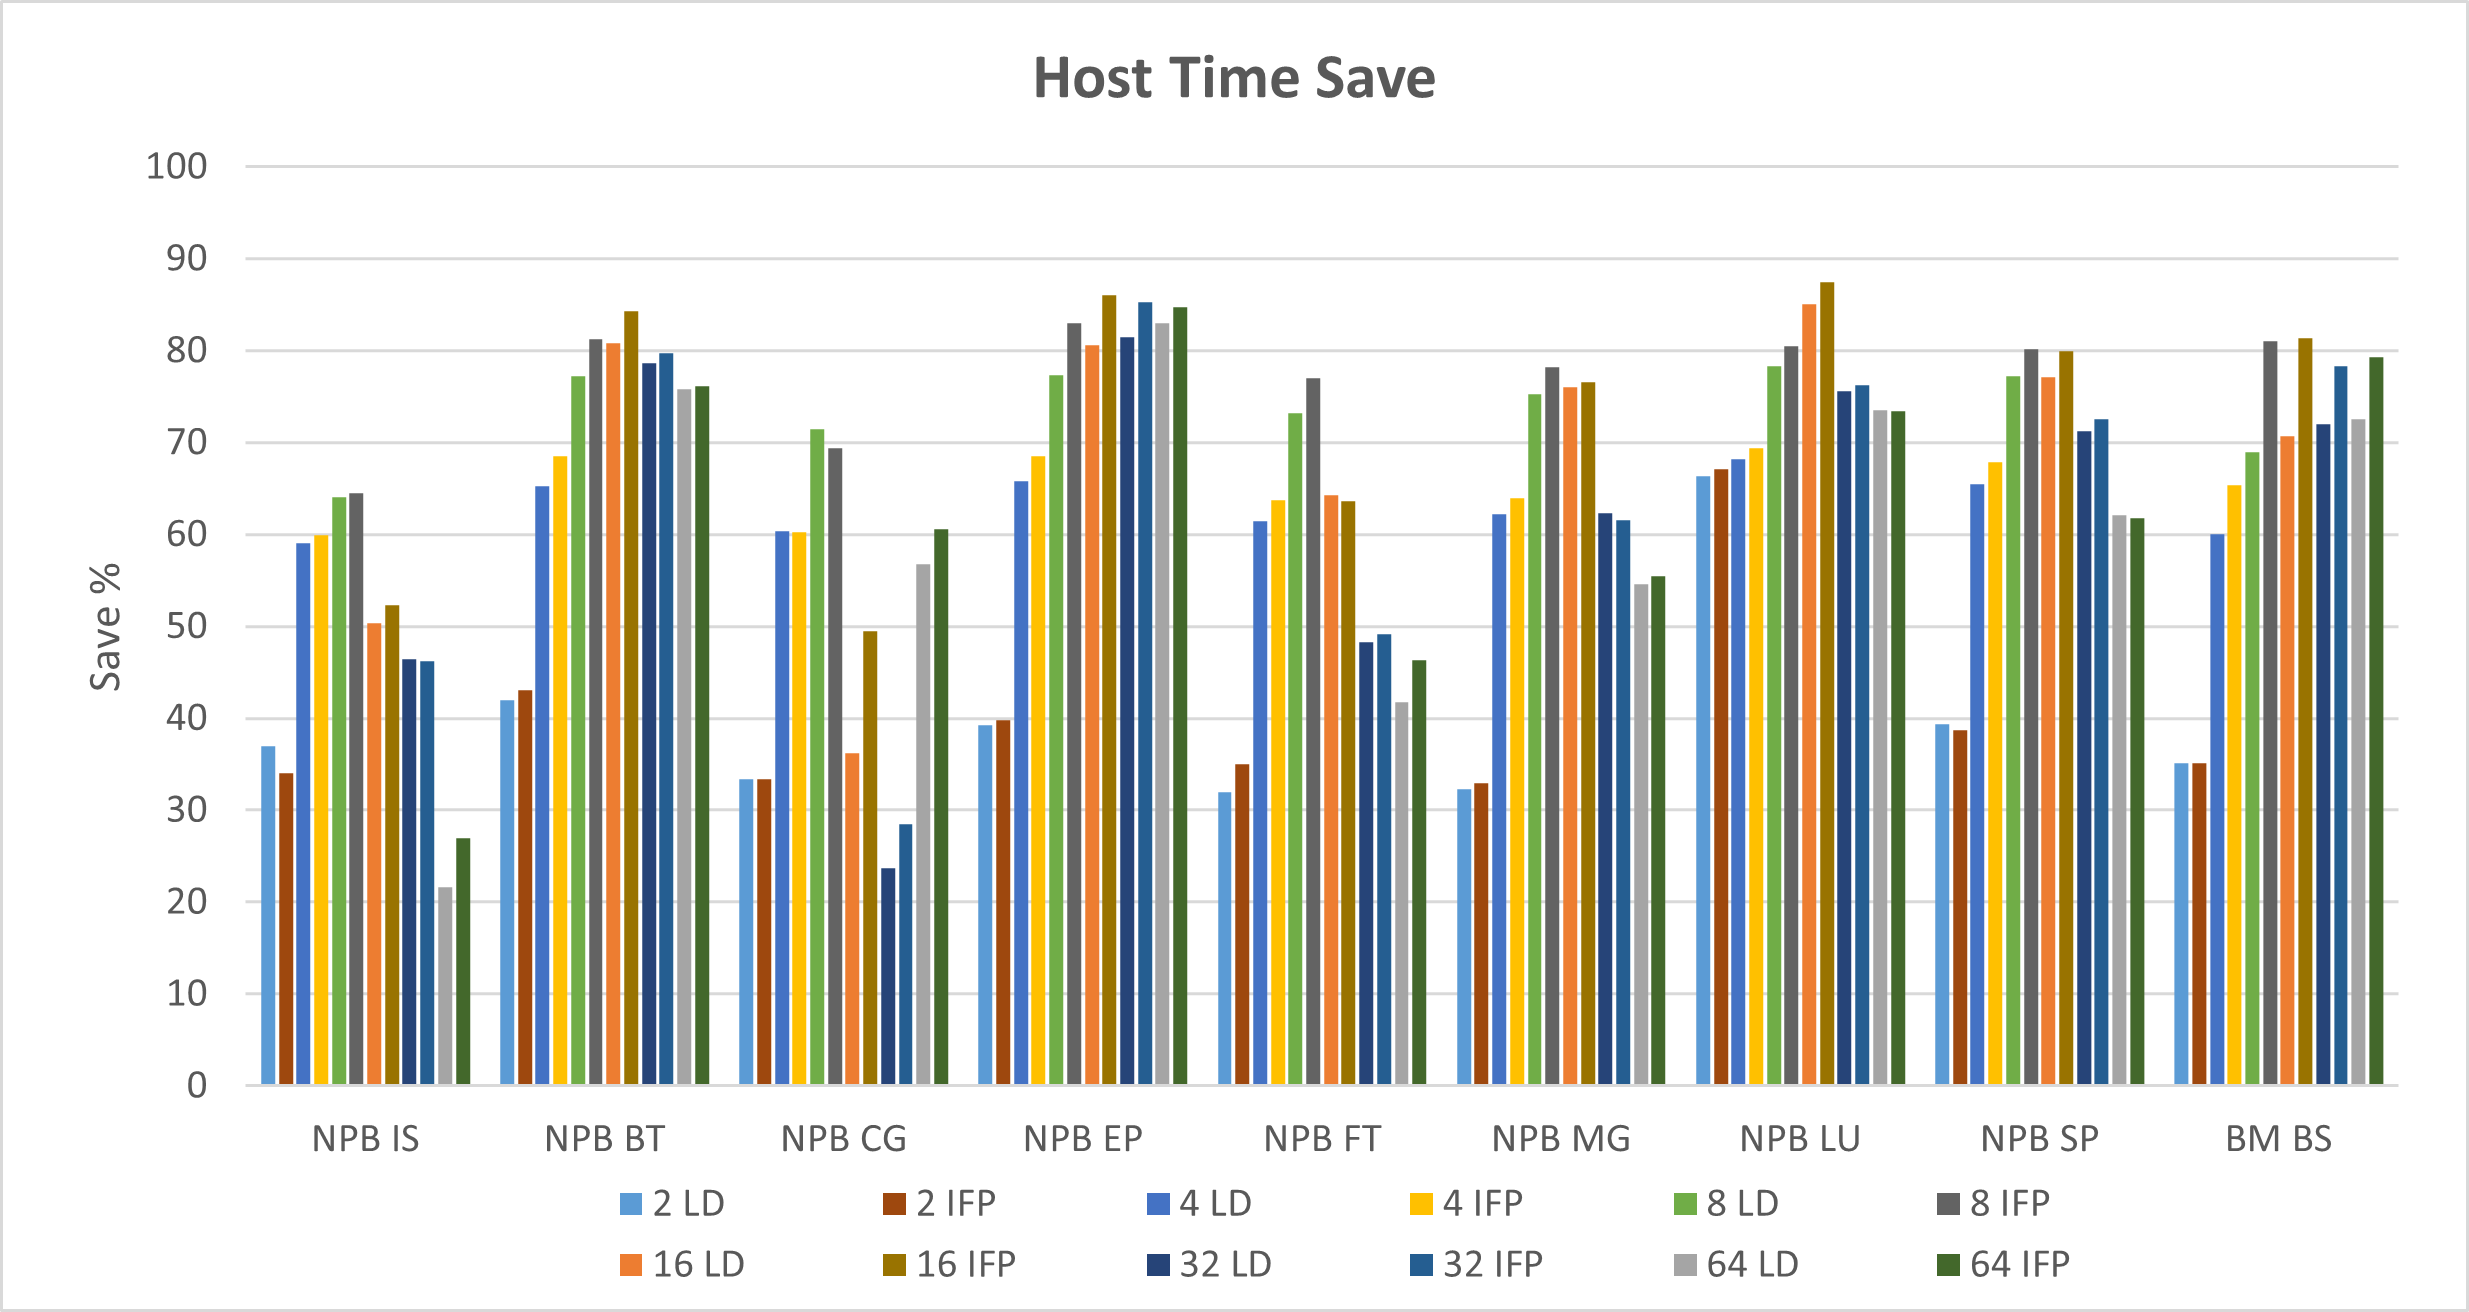
\includegraphics[width=0.8\textwidth]{Images/Host_REP.png}
    \caption{ Host time save}
    \label{fig:Host_ADAINCPCREP}
\end{subfigure}
        
\caption{Loop Detection algorithm results}
\label{fig:results_ADAINCPCREP}
\end{figure}

Performance, and consequently, host time were the ones that experienced the most decline. Nearly every simulated scenario exhibited it, 
with particular emphasis on the NPB EP case, where the loss was around 97\%. Overall, the performance drop was, on average, almost 40\%, 
representing in host time, also on average, a reduction of 3\%. Although it is a small value compared to the previous one, it can reflect a huge 
difference, like the case of NPB LU with 16 simulated cores. In percentage, the host time difference is almost 2.5\% however, 
the actual time difference is 1433 seconds, that is, almost 24 minutes. 

On the accuracy side, the gains were not as evident as expected. In some cases, there was a growth in the inaccuracy, having inclusively overpassed
the 5\% limit in the two cases. There are also others where there was a reduction, for example, the NPB FT with 16 cores and the NPB MG with 32 
cores. Negative inaccuracy is still present due to the exposed reasons in the section \ref{sec:ADALINE_results}. 

In the final analysis, the performance sacrifice does not reflect a relevant gain in accuracy. Nevertheless, there is one case, NPB CG, where until 
eight simulated cores, the performance was a little bit better than the approach presented in the last section. Concerning this exception, a deeper look 
was done at this benchmark using perf, a performance analysis tool for Linux that provides a framework for both hardware and software-level 
features. After analysing the NPB CG, the result present in the \autoref{fig_NPBCG_CycleAnalysis} was obtained. 

\begin{figure}[H]
    \begin{subfigure}{\textwidth}
        \centering
        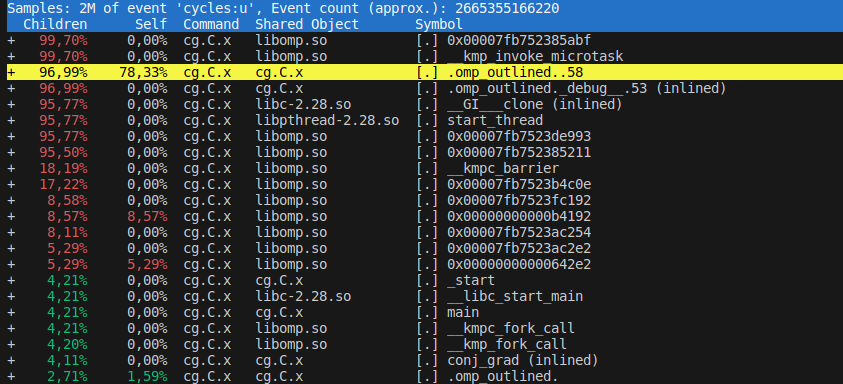
\includegraphics[width=0.7\textwidth]{Images/NPBCG_CycleAnalysis.png}
        \caption{ Performance analysis}
        \label{fig_NPBCG_CycleAnalysis}
    \end{subfigure}
    \begin{subfigure}{\textwidth}
        \centering
        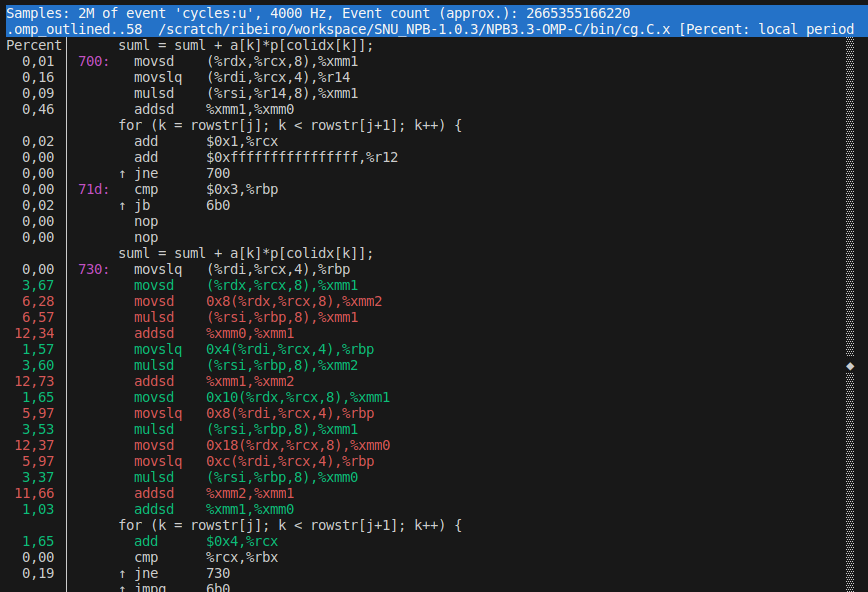
\includegraphics[width=0.6\textwidth]{Images/NPBCG_MostTimeSpentRegion.png}
        \caption{ Region of greatest time cost}
        \label{fig_NPBCG_MostTimeSpentRegion}
    \end{subfigure}
    \caption{Perf analysis on NPB CG}
\end{figure}

It is evident that there is a specific part within this benchmark where the simulator consumes the major processing time. This part is 
exposed in the \autoref{fig_NPBCG_MostTimeSpentRegion}. If all percentages that are associated with an instruction with a green or red color 
were summed, the outcome would be nearly 94\% of time spent. Examining the benchmark's source code can be identified the previous region, which is 
shown below. 


\begin{lstlisting}[style=customC, caption={Snippet source code of NPB CG}, label=CodeNpbCgSnippet]
//---------------------------------------------------------------------
//  q = A.p
//  The partition submatrix-vector multiply: use workspace W
//---------------------------------------------------------------------
for (cgit = 1; cgit <= cgitmax; cgit++) 
{
    //...//

    for (j = 0; j < lastrow - firstrow + 1; j++) 
    {
        sum = 0.0;

        for (k = rowstr[j]; k < rowstr[j+1]; k++) 
        {
            sum = sum + a[k]*p[colidx[k]];
        }

        q[j] = sum;
    }

    //...//
}
\end{lstlisting}

Upon the code examination, it is evident that three nested loops perform repetitive tasks. In other words, there are no conditional 
statements to modify the workflow path, which does not happen on the remaining benchmarks. Thereby, it can be stated that this type of 
workload takes advantage of this approach, obtaining better results. For this reason, this algorithm should not be discarded, as potential 
future optimizations for specific tasks may necessitate this approach.

\section{Improved Baseline Algorithm}
\label{subsec::finalAlgorithm}

After the development and testing of all aforementioned algorithms, it was determined the better approach is the combination of the ADALINE-based, 
the dynamic increment, and the \gls{pc} analyses. The results show they complement each other, providing a great trade-off between performance 
and accuracy. The repetition algorithm was not integrated into the final solution due to its weak performance and accuracy gain. 

The synchronization process can now be redefined to integrate the dynamic approach, as illustrated in the following flowchart. 
The static version was not removed because, with a-priory information about the benchmark, 
the best quantum can be calculated before simulating. One example is a network application, where the communications delays are well-defined. 
If the quantum is set with the smaller delay, a perfect accuracy can be achieved \cite{dist-gem5}. 

\begin{figure}[H]
	\centering
 	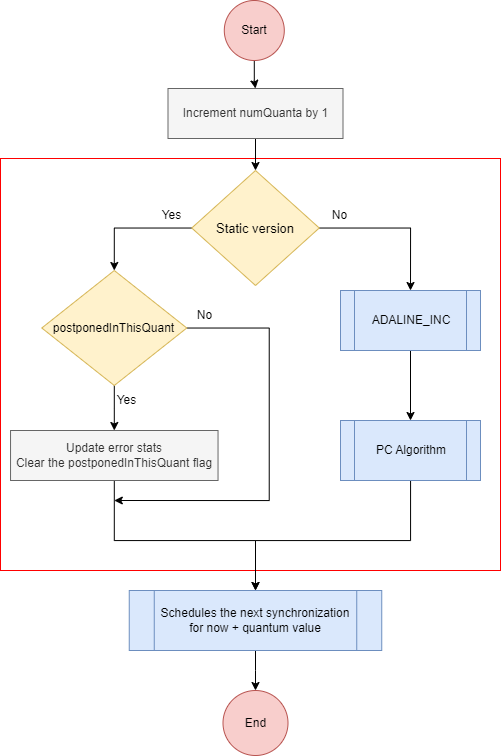
\includegraphics[width=0.4\linewidth]{Images/NewGlobalSyncEventStatic.png}
 	\caption{New quantum definition in the synchronization process}
	\label{fig_NewGlobalSyncEventStatic}
\end{figure}

\subsection{Results}

The next graphs present a comparison between the improved baseline algorithm and the static mode with one microsecond synchronization time. 

\begin{figure}[H]
    \centering
    \begin{subfigure}{\textwidth}
        \centering
        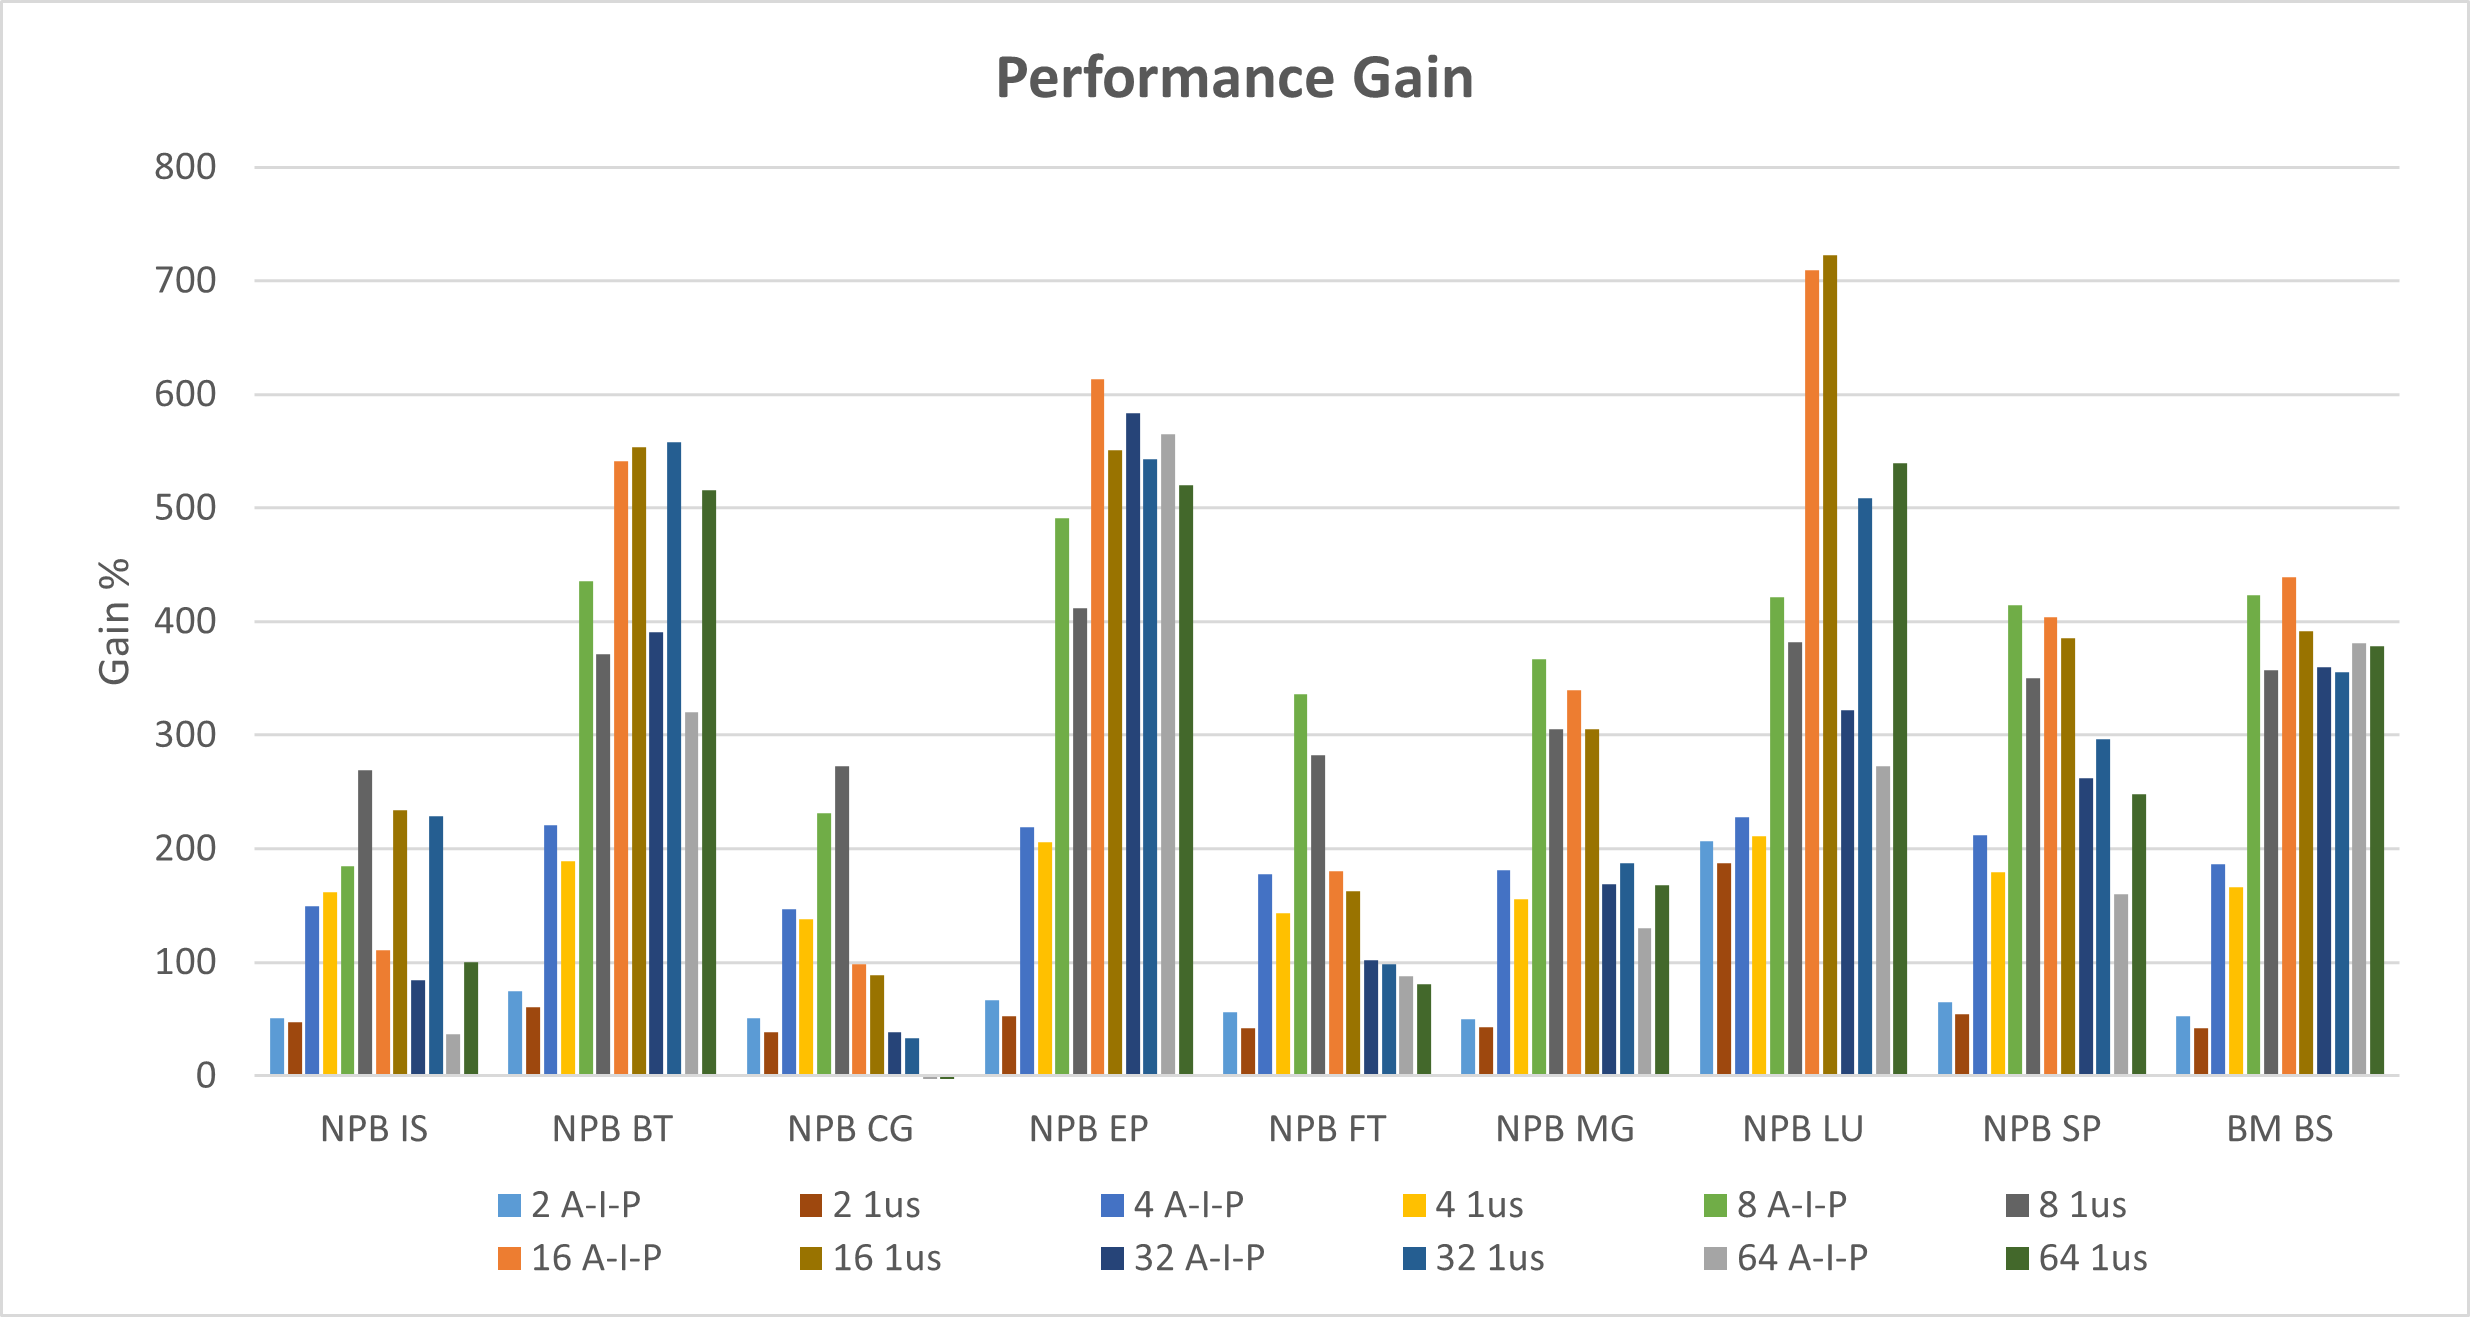
\includegraphics[width=0.82\textwidth]{Images/Performance_FINAL.png}
        \caption{ Performance gain}
        \label{fig:Performance_FINAL}
    \end{subfigure}
    \begin{subfigure}{\textwidth}
        \centering
        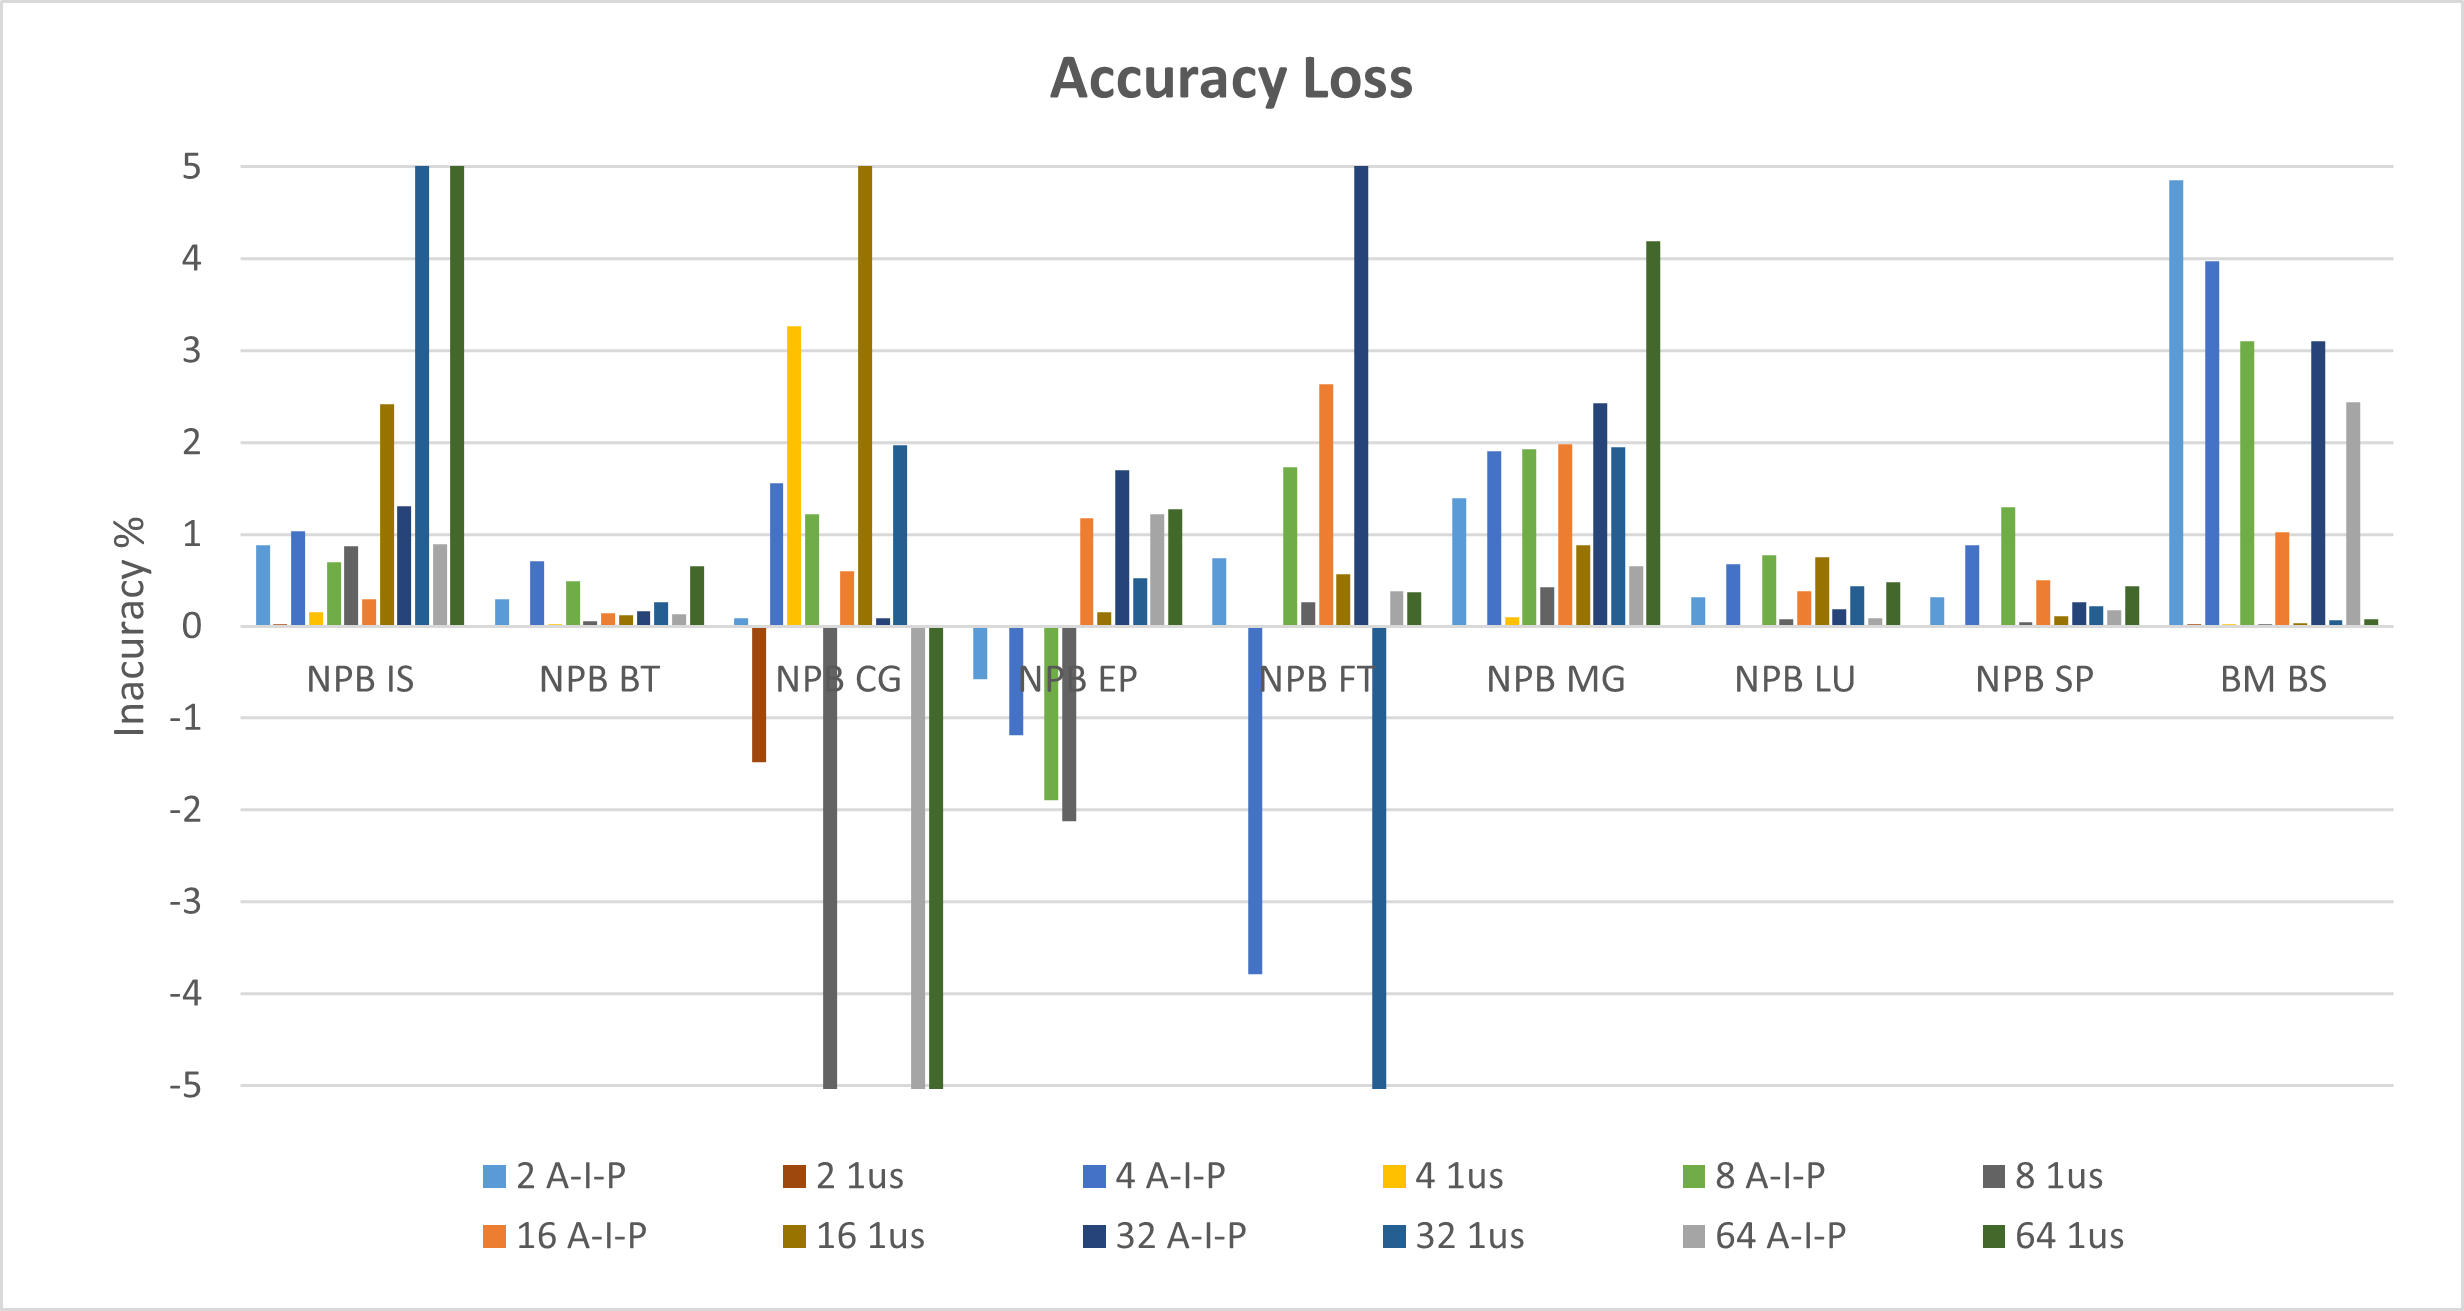
\includegraphics[width=0.82\textwidth]{Images/Accuracy_FINAL.png}
        \caption{ Accuracy lost}
        \label{fig:Accuracy_FINAL}
    \end{subfigure}
    \begin{subfigure}{\textwidth}
        \centering
        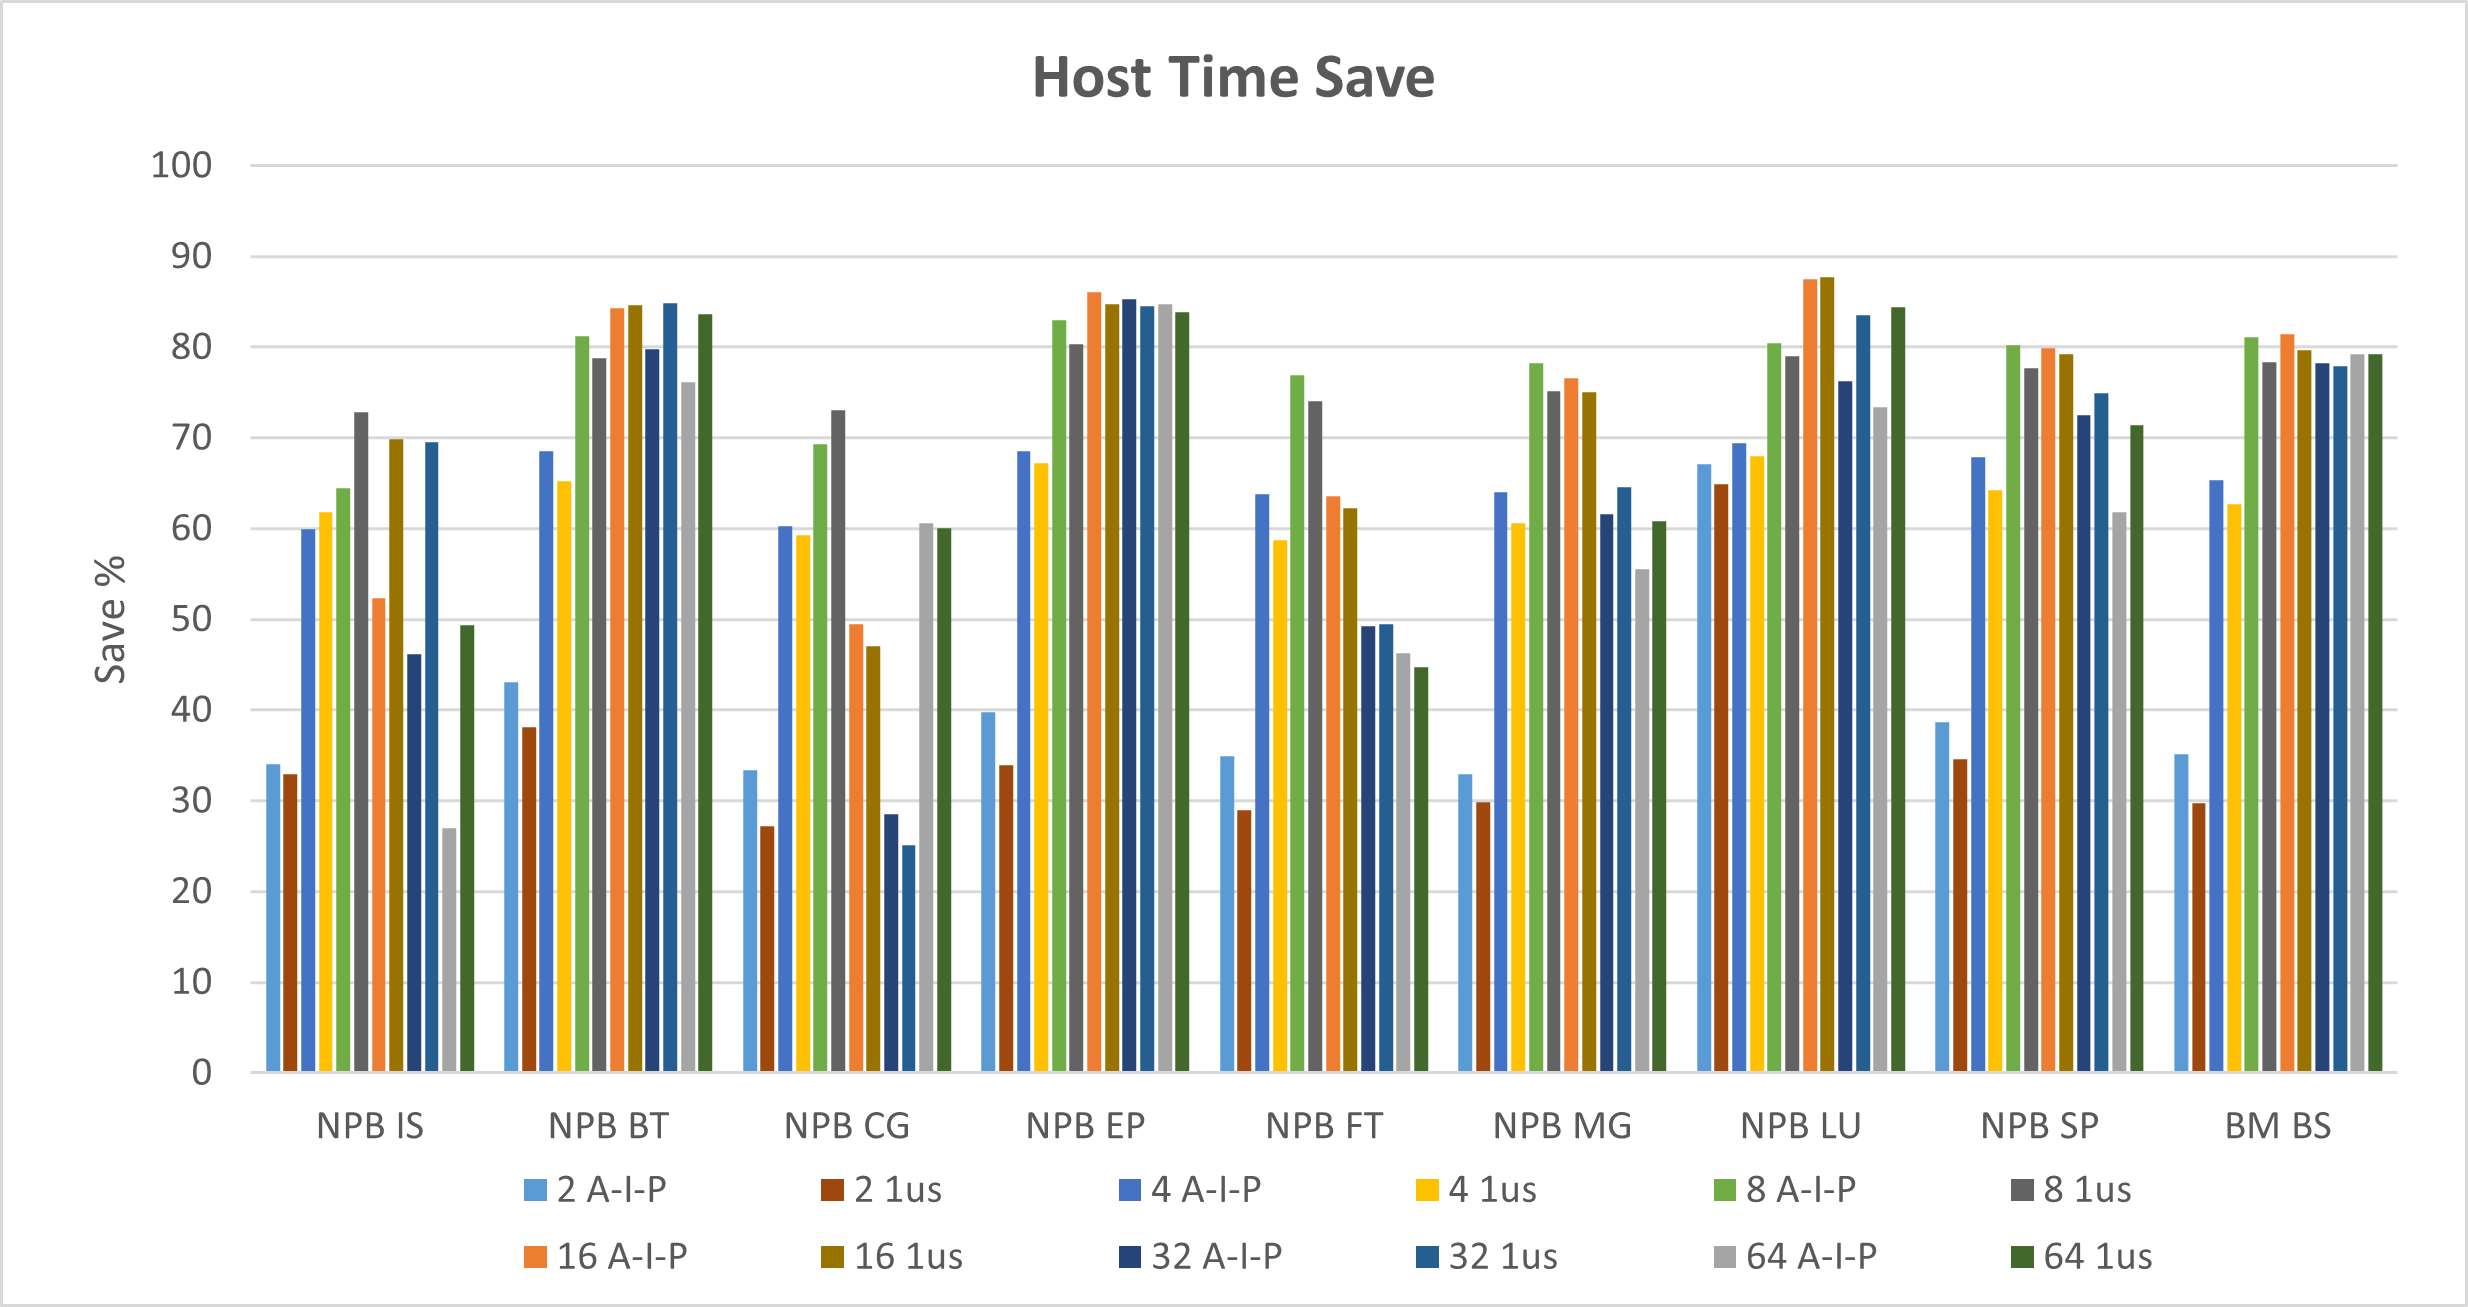
\includegraphics[width=0.82\textwidth]{Images/Host_FINAL.png}
        \caption{ Host time save}
        \label{fig:Host_FINAL}
    \end{subfigure}

\caption{Improved baseline and static mode comparison}
\label{fig:results_FINAL}
\end{figure}


Starting with performance, the dynamic version outperformed the other one in most of the cases. Nevertheless, in the cases where it 
did not happen, in particular, NPB BT, LU, and SP with 32 and 64 simulated cores, the performance difference was huge. 
This is related to the Step Ladder design, as previously explained in this chapter. 
If the previous cases are considered,
when calculating the mean of performance gain and comparing it with the static version, the result would be circa -9\%. Without the previous 
tests, the gain average would be almost 10\%. 

Moving to accuracy, in all workloads, the dynamic approach only exceeded the 5\% inaccuracy in two cases. On the other hand, the static 
version performed worst, having six occurrences. In the remaining cases, on average, there was an increment of 0.5\% of inaccuracy when 
using the developed algorithm. As previously discussed, the issue of negative inaccuracy persists in both approaches, as has been observed thus far.

It is important to mention that, in the dynamic case, all of these occurrences are related to 
simulation issues inherent in par-gem5 nature. Going into detail, the sum/subtraction of the sequential target time with the 
worst-case scenario may give a smaller/higher value than the obtained target time. \autoref{fig_pargem5_Issue} demonstrates the previously described 
scenario. The target time obtained must be within the maximum inaccuracy, which sometimes does not verify. In these cases, the simulation result 
should not be considered, and since both fit in this scenario, the dynamic version occurrences were discarded. Meanwhile, the static 
version exhibited similar cases as well, with two of six representing this particular situation. 

\begin{figure}[H]
    \centering
    \begin{subfigure}{\textwidth}
        \centering
        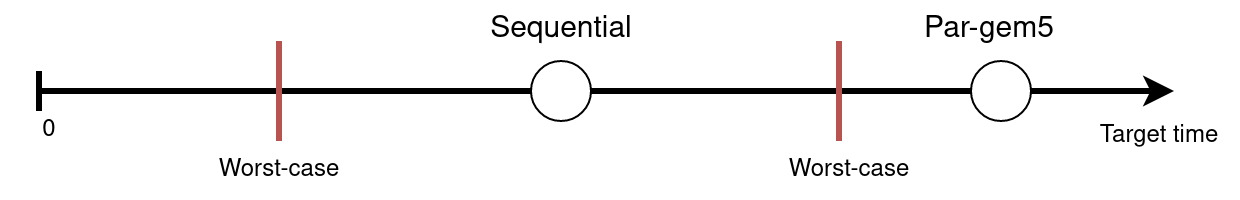
\includegraphics[width=0.8\textwidth]{Images/pargem5_Issue1.png}
    \end{subfigure}
    \begin{subfigure}{\textwidth}
        \centering
        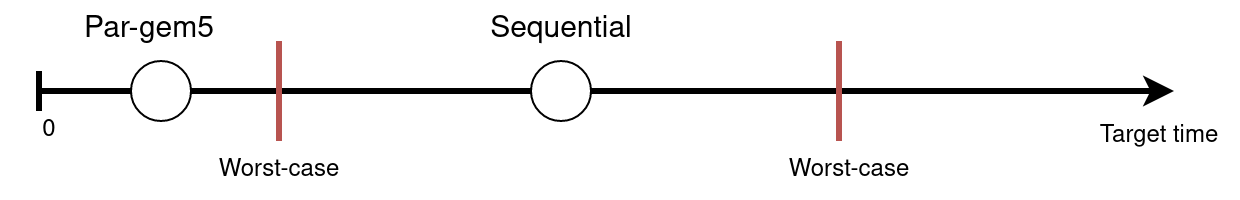
\includegraphics[width=0.8\textwidth]{Images/pargem5_Issue2.png}
    \end{subfigure}

    \caption{Simulation issue in par-gem5}
	\label{fig_pargem5_Issue}
\end{figure}

Finally, in terms of host time, the results are again very positive for the dynamic version. Until 4 simulated cores, only one case did not 
show improvements, and in the left cases, the major part show also gains. There are still situations where it does not verify, 
especially when 32 and 64 simulated cores. However, it is crucial to emphasize that accuracy should exceed 95\%, a criterion that is 
not met in certain cases, such as NPB IS.




% \subsection{CPU model}

% To understand how can the prediction be made, it is important to understand the \gls{cpu} model in use. At the moment, 
% par-gem5 \cite{pargem5} is restricted to the AtomicSimpleCPU model, which means is simpler and faster than the other versions. Nevertheless, 
% the accuracy is sacrificed, because there is no verification, as presented in the \autoref{fig_AtomicMode}. The following image presents in 
% detail its execution process.

% \begin{figure}[H]
% 	\centering
%  	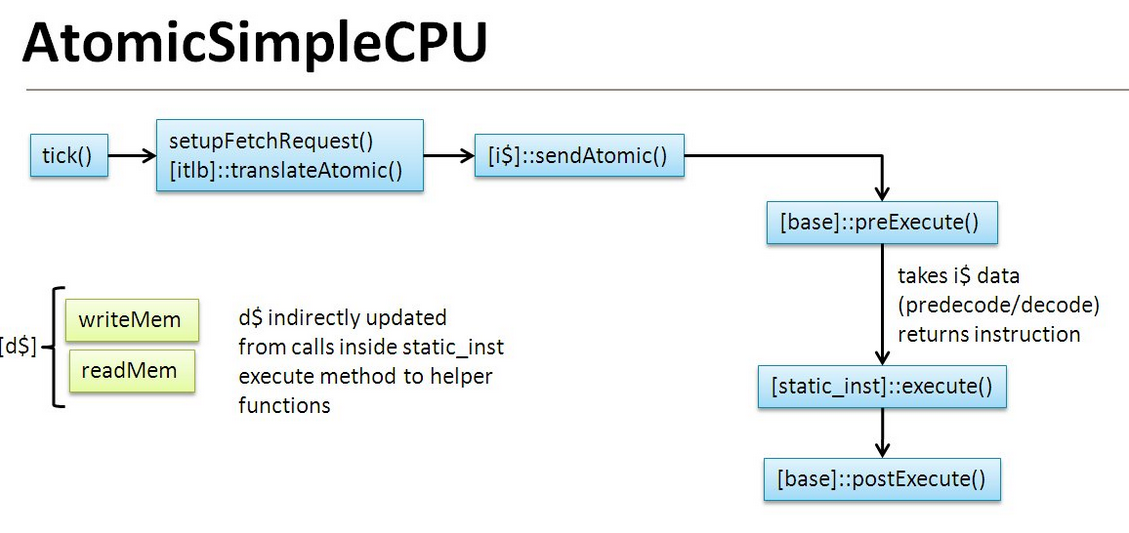
\includegraphics[width=0.7\linewidth]{Images/AtomicSimpleCPU.png}
%  	\caption{AtomicSimpleCPU execution process}
% 	 \label{fig_AtomicSimpleCPU}
% \end{figure}

% The tick event is responsible for stimulating the simulation

% %figure do atomic e explaicar onde deve de ser aplicado a deteçao.


%The algorithm's design must be flexible, in a way that benchmarks can have the best performance within accuracy limits. 